Introduce top-tagging study, cite earlier studies of top tagging.

\subsection{Methodology}
We examine a number of top-tagging strategies. The taggers attempt to reconstruct the top and $W$ mass for a candidate boosted top. We consider
%
\begin{enumerate}
\item HEPTopTagger
\item Johns Hopkins Tagger (JH)
\item Trimming
\item Pruning
\end{enumerate}
%
The grooming algorithms (trimming and pruning) do not automatically incorporate a $W$-identification step. For a level playing field, we construct a $W$ candidate from the three leading subjets by taking the pair of subjets with the smallest invariant mass.

We also consider the above taggers supplemented with jet shape information. In particular, we consider $N$-subjettiness ratios $\tau_{32}^{\beta=1}$ and $\tau_{21}^{\beta=1}$, energy correlation function ratios $C_3^{\beta=1}$ and $C_2^{\beta=1}$, and the Qjet mass volatility $\Gamma$.

To determine the performance of each tagger, we combine the tagger output observables and jet shapes into a boosted decision tree (BDT), which determines the optimal multivariable cut. Additionally, because each tagger has two inputs (list, or maybe refer back to Section 3), we scan over reasonable values of the inputs to determine the optimal value for each top tagging signal efficiency. This allows us a direct comparison of the optimized version of each tagger. 

\subsection{Performance at moderate boost}

\begin{figure*}
\begin{center}
\subfigure[HEPTopTagger]{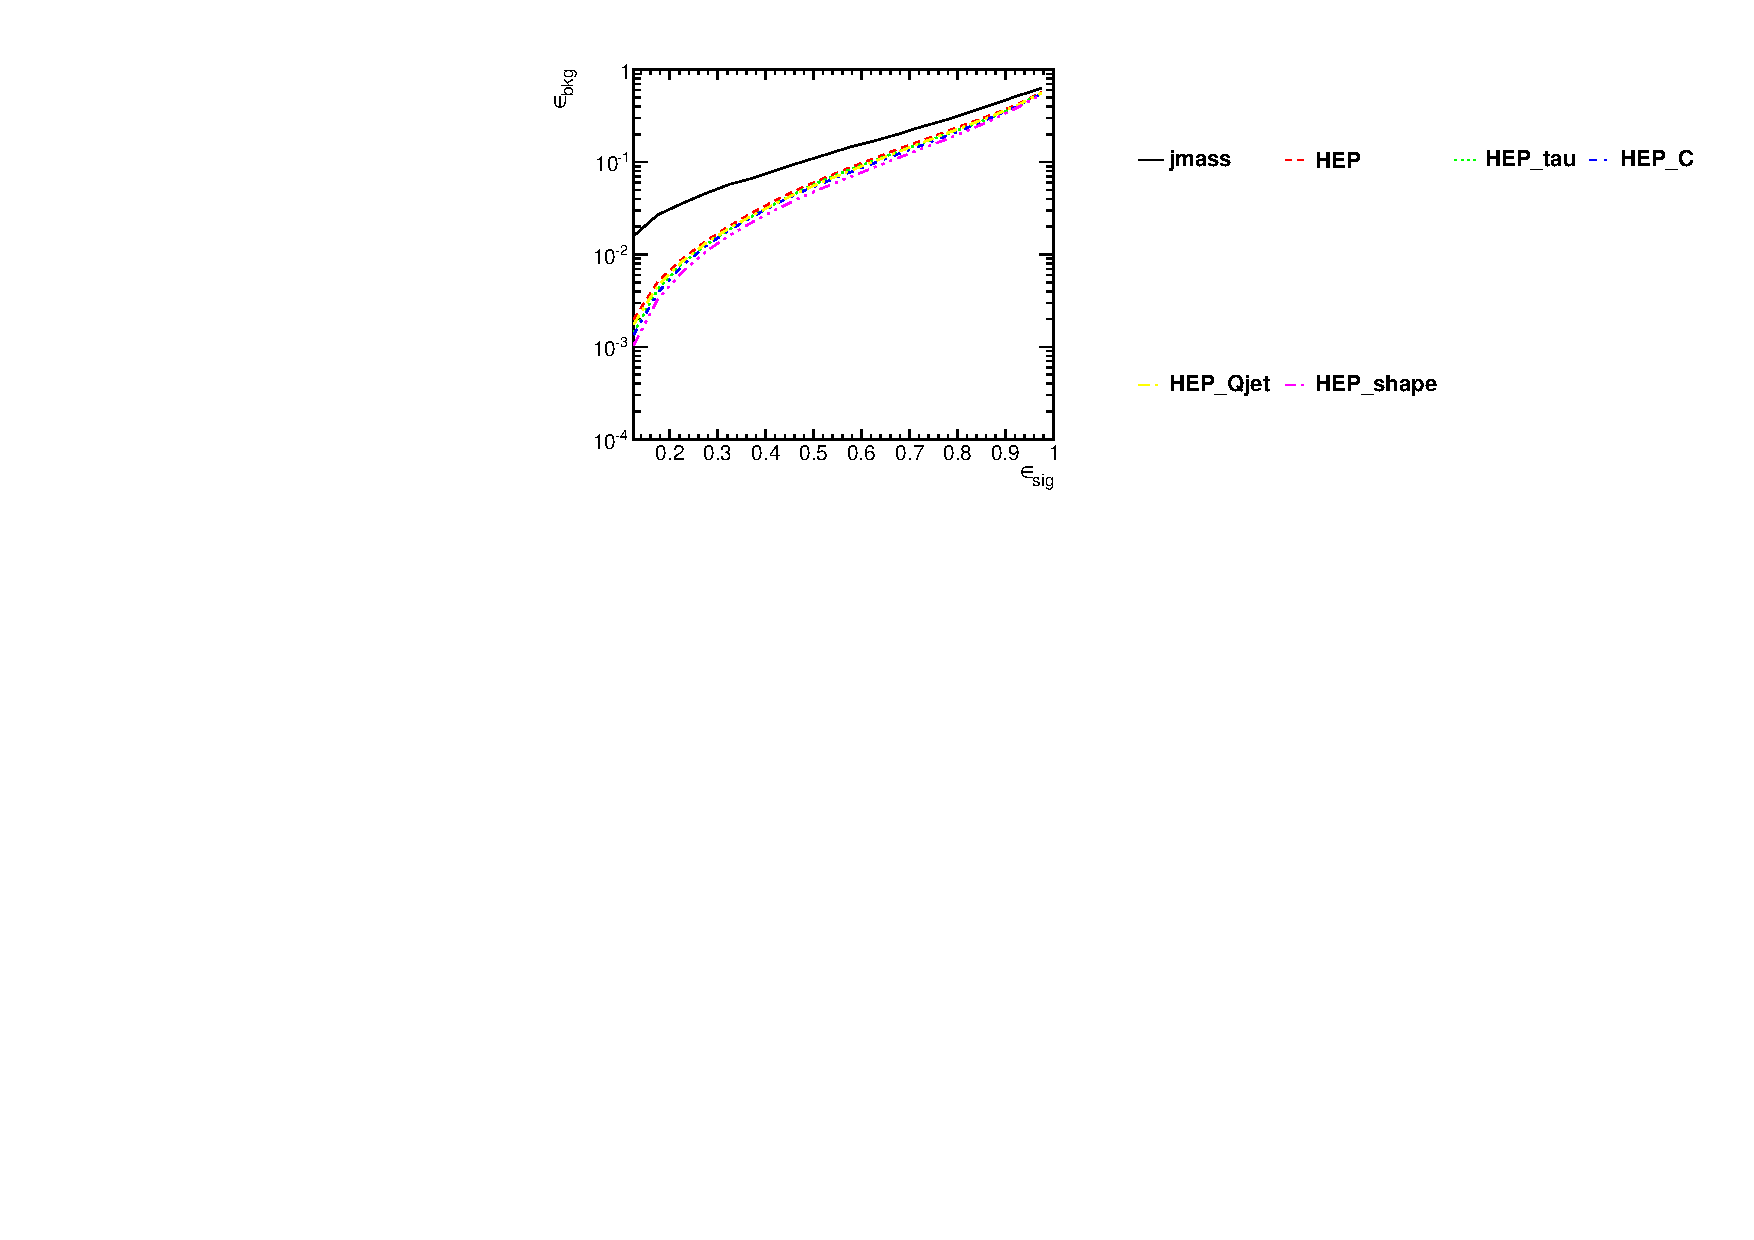
\includegraphics[width=0.48\textwidth]{./Figures/TTagging/0p5TeV_0p8/Rocs_HEP_few.pdf}}
\subfigure[Johns Hopkins Tagger]{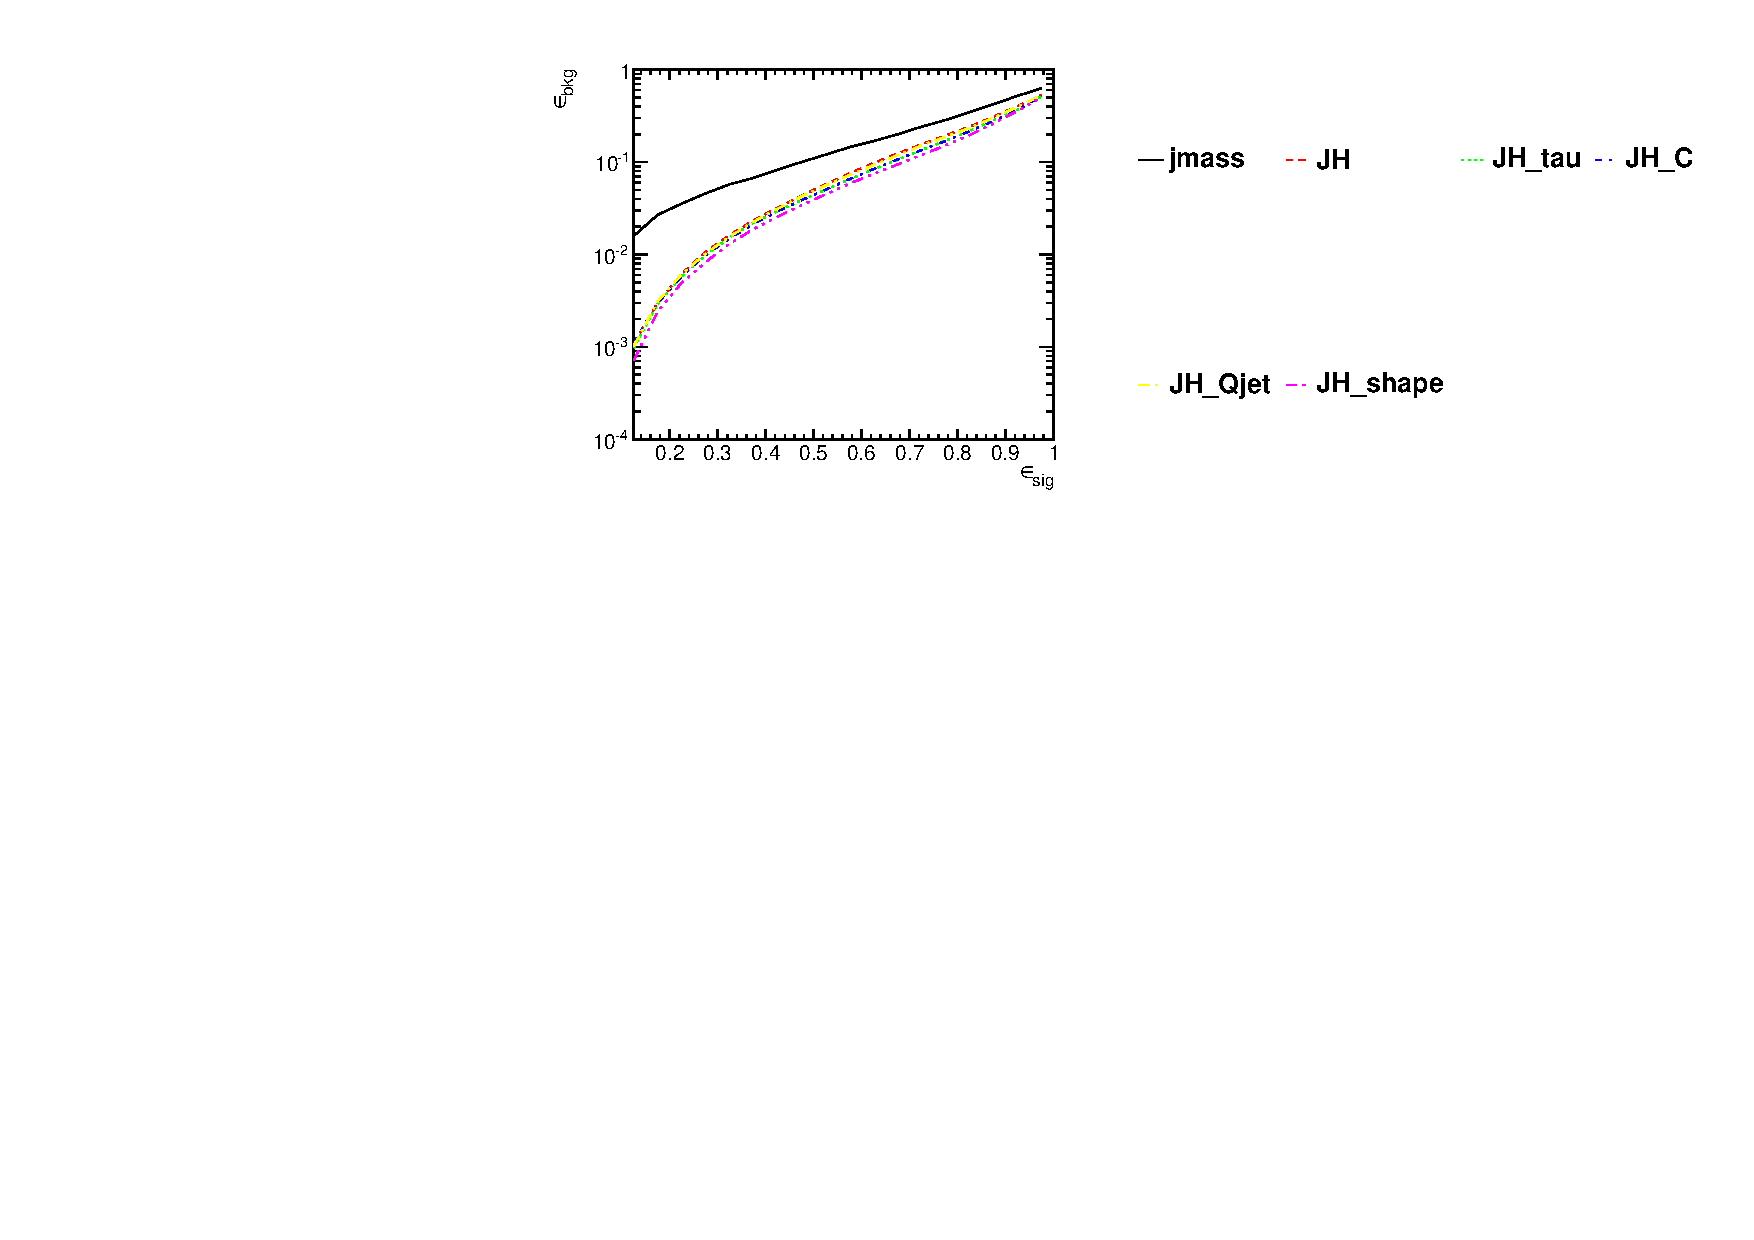
\includegraphics[width=0.48\textwidth]{./Figures/TTagging/0p5TeV_0p8/Rocs_JH_few.pdf}}
\subfigure[Pruning]{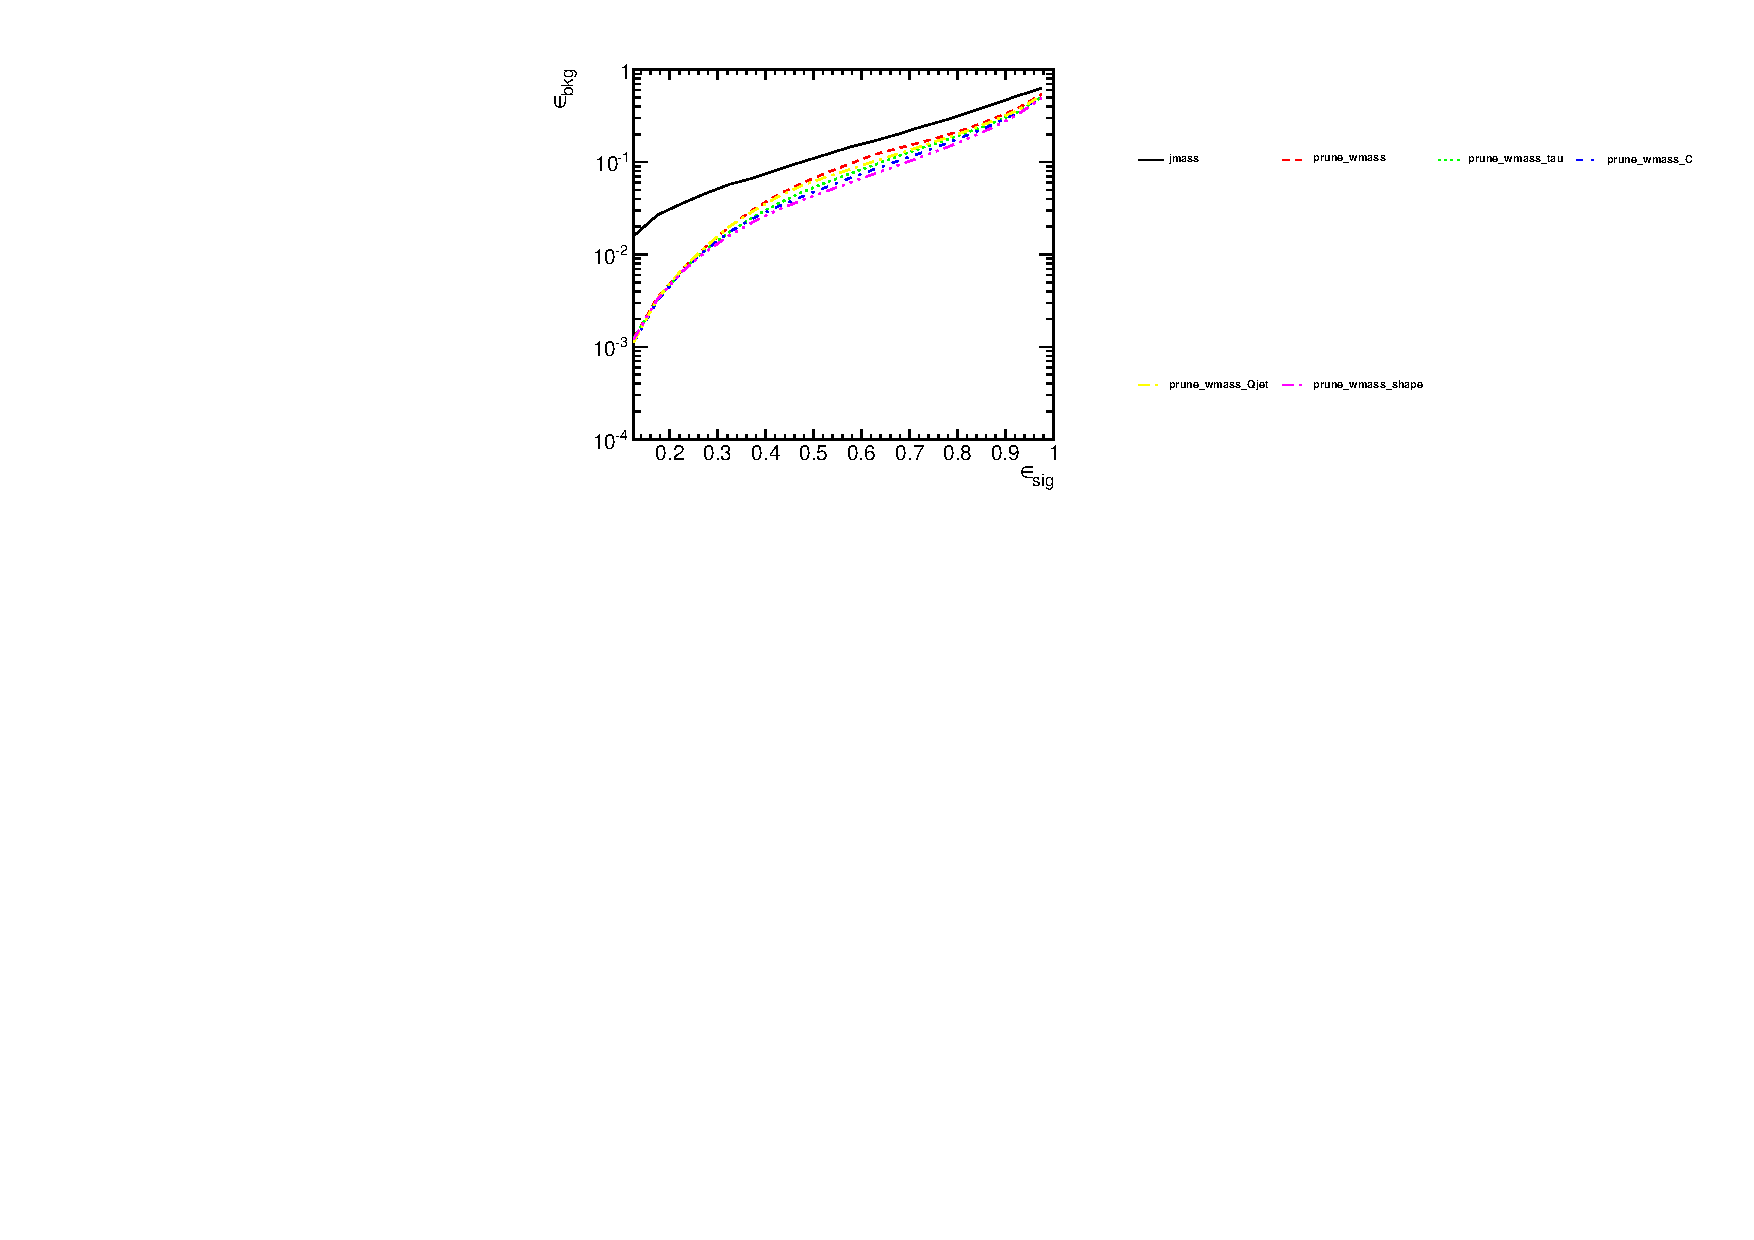
\includegraphics[width=0.48\textwidth]{./Figures/TTagging/0p5TeV_0p8/Rocs_prune_few.pdf}}
\subfigure[Trimming]{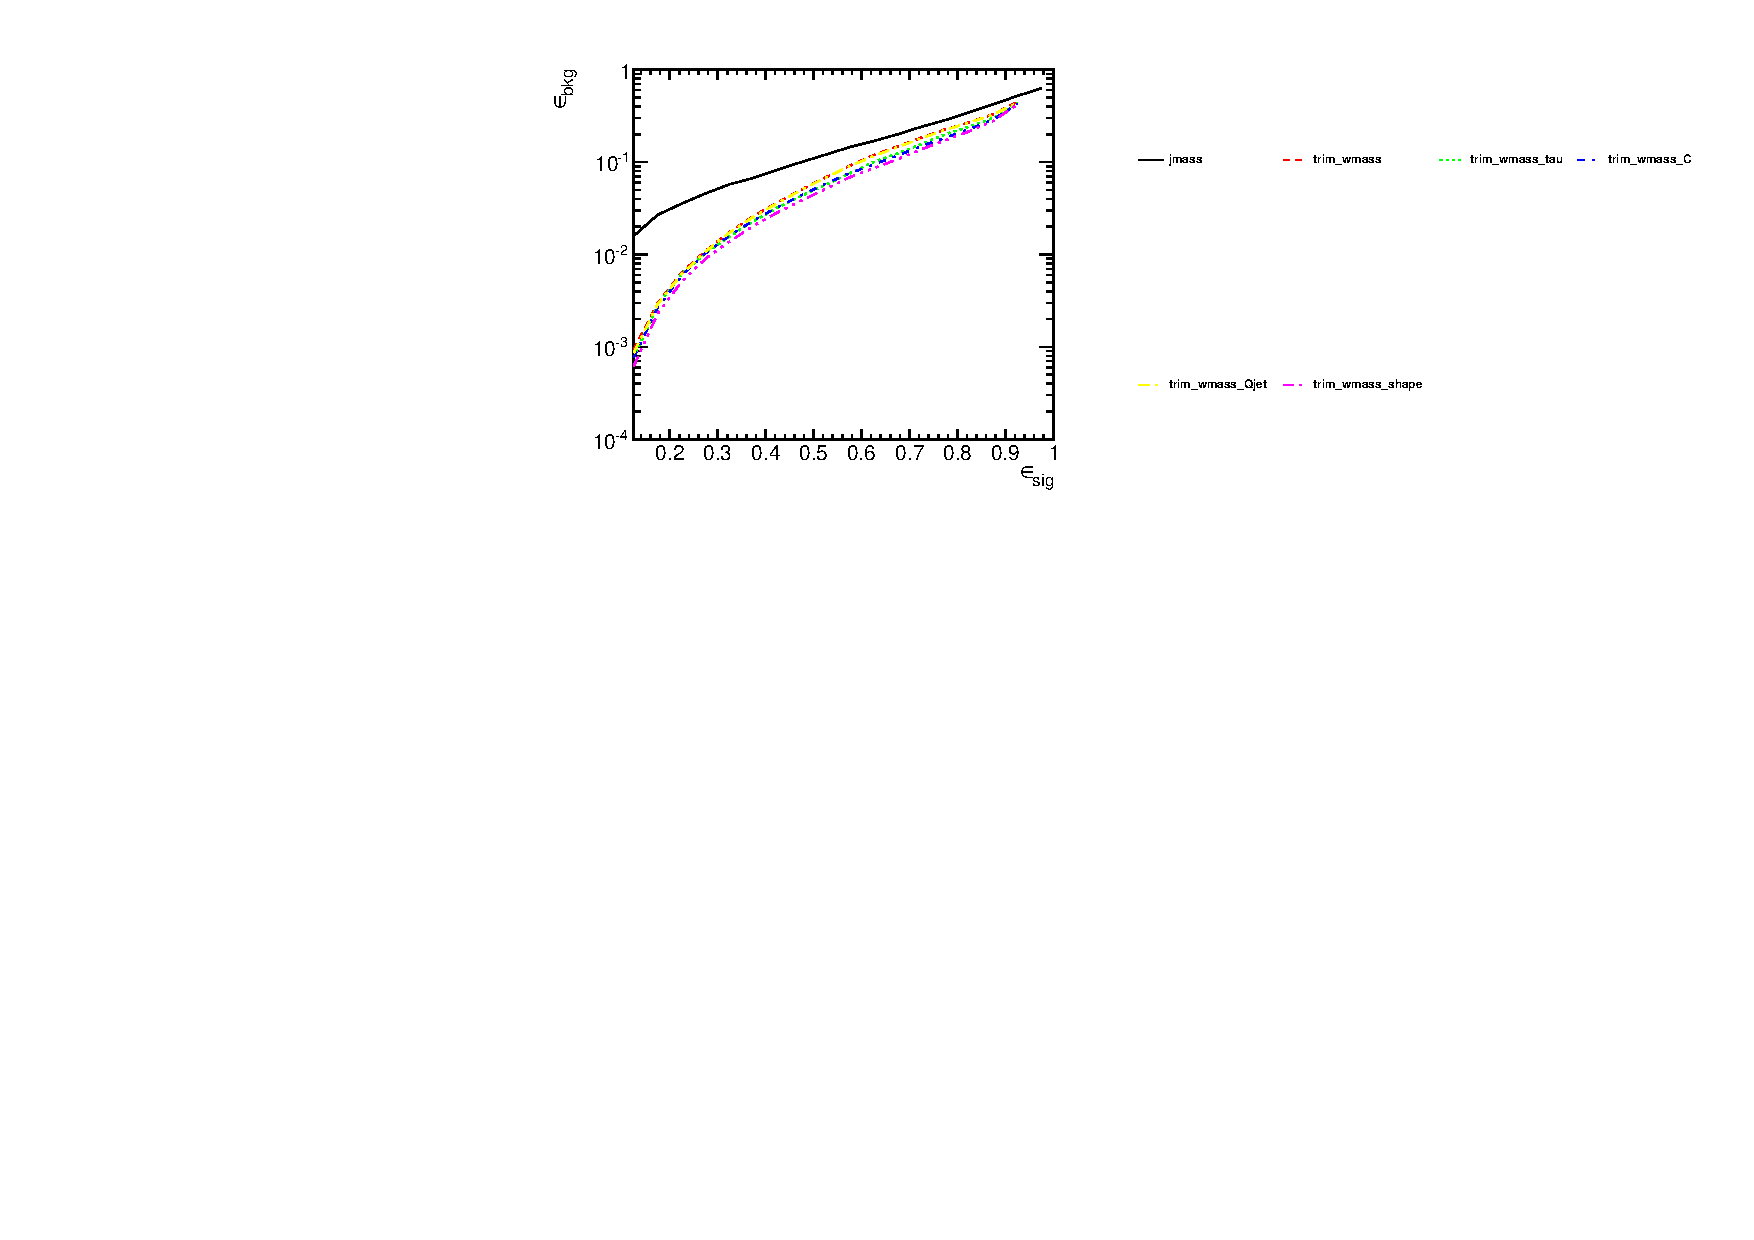
\includegraphics[width=0.48\textwidth]{./Figures/TTagging/0p5TeV_0p8/Rocs_trim_few.pdf}}
\subfigure[HEP+JH comparison]{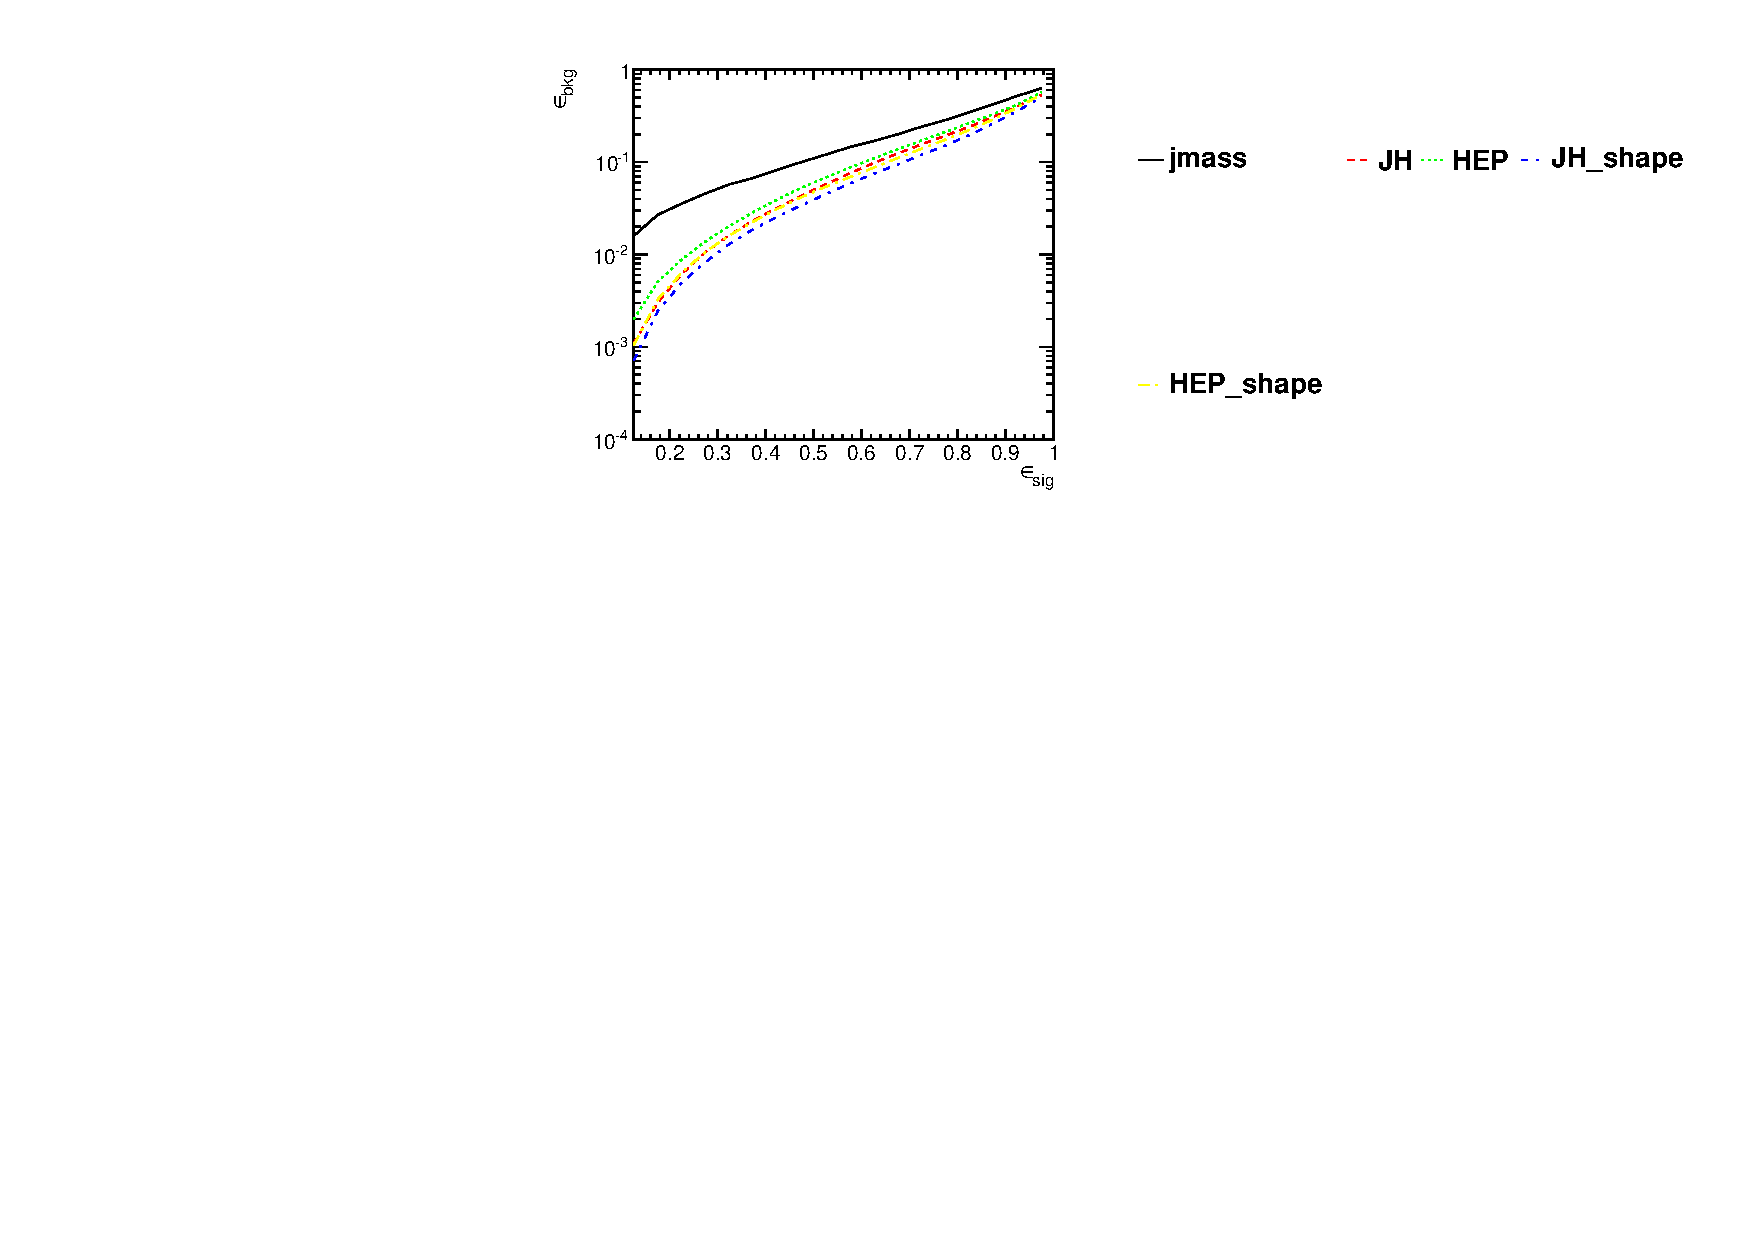
\includegraphics[width=0.48\textwidth]{./Figures/TTagging/0p5TeV_0p8/Rocs_tagger_shape_few.pdf}}
\subfigure[Grooming comparison]{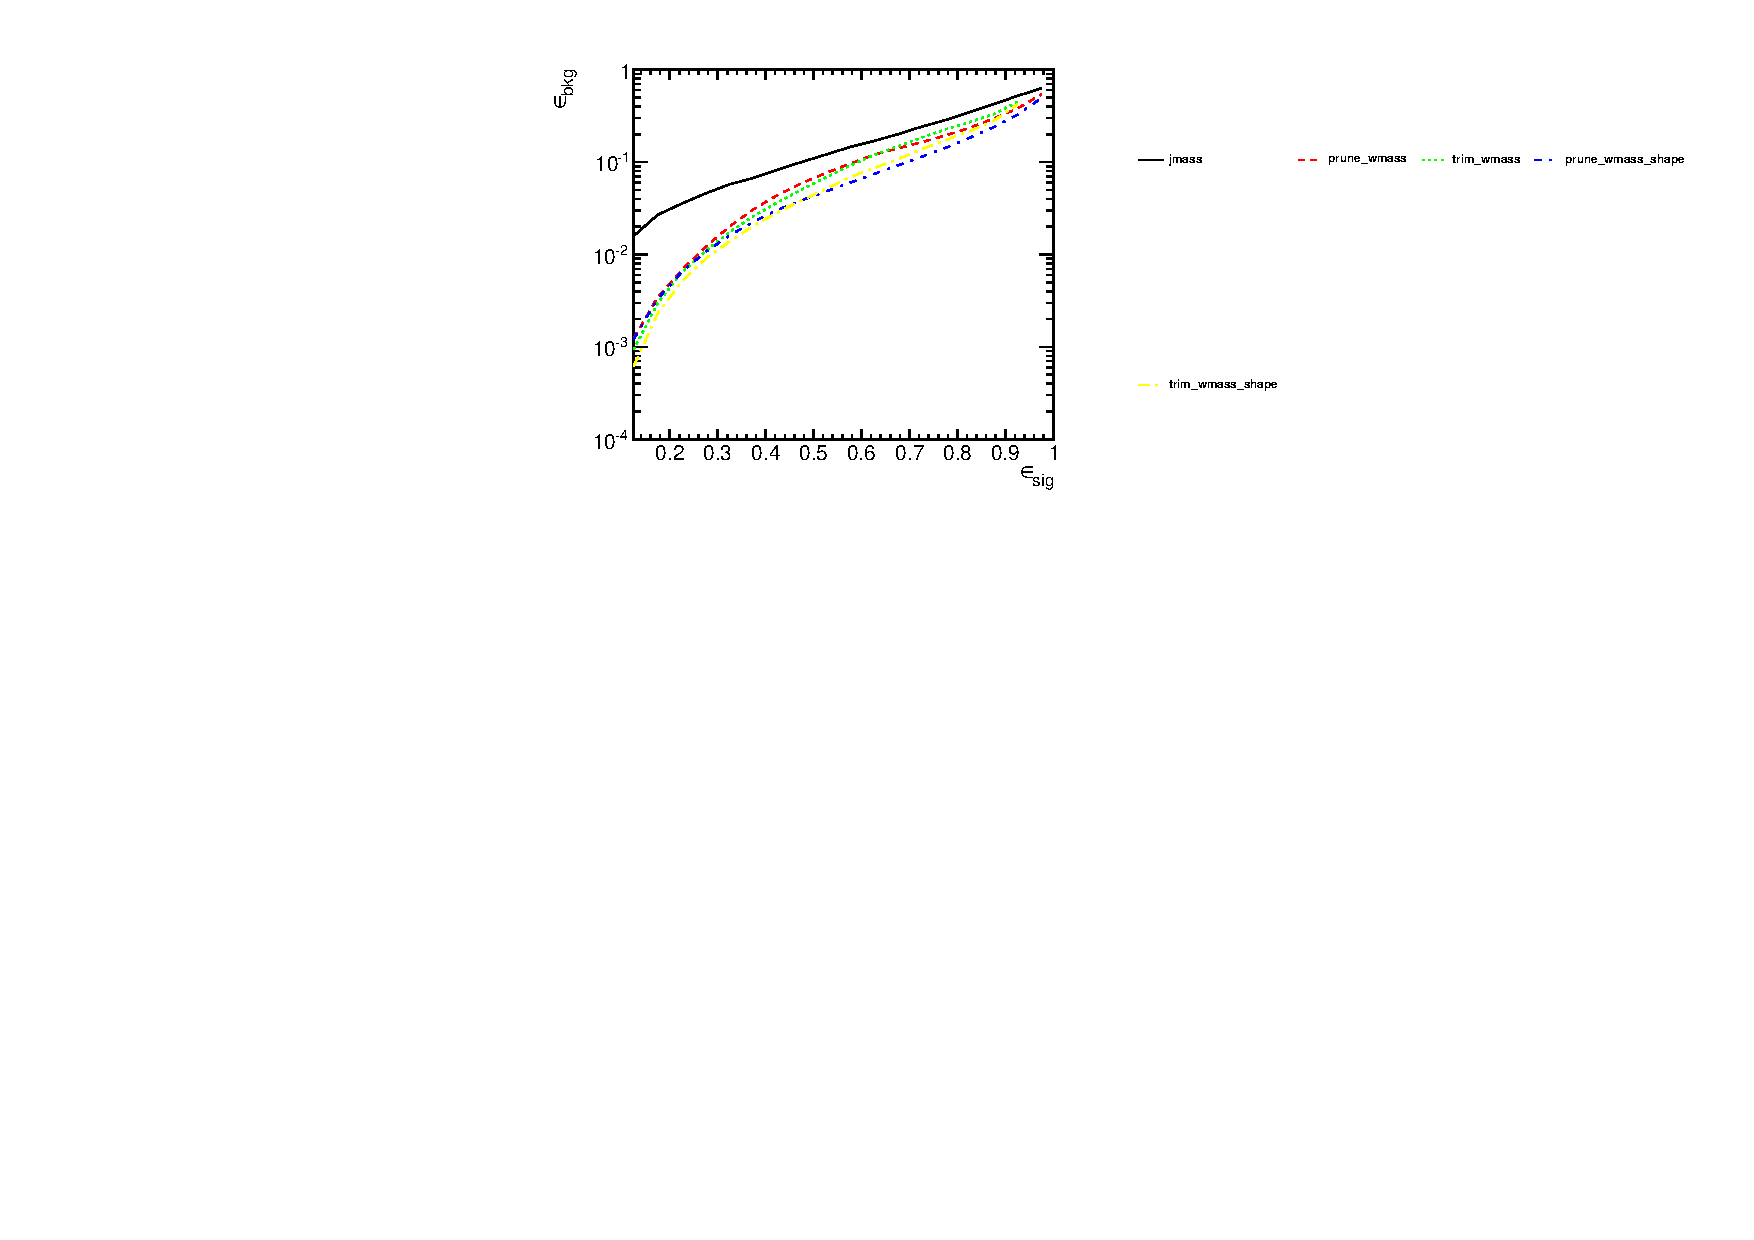
\includegraphics[width=0.48\textwidth]{./Figures/TTagging/0p5TeV_0p8/Rocs_groom_shape_few.pdf}}
\subfigure[Comparison of Tagger+Shape]{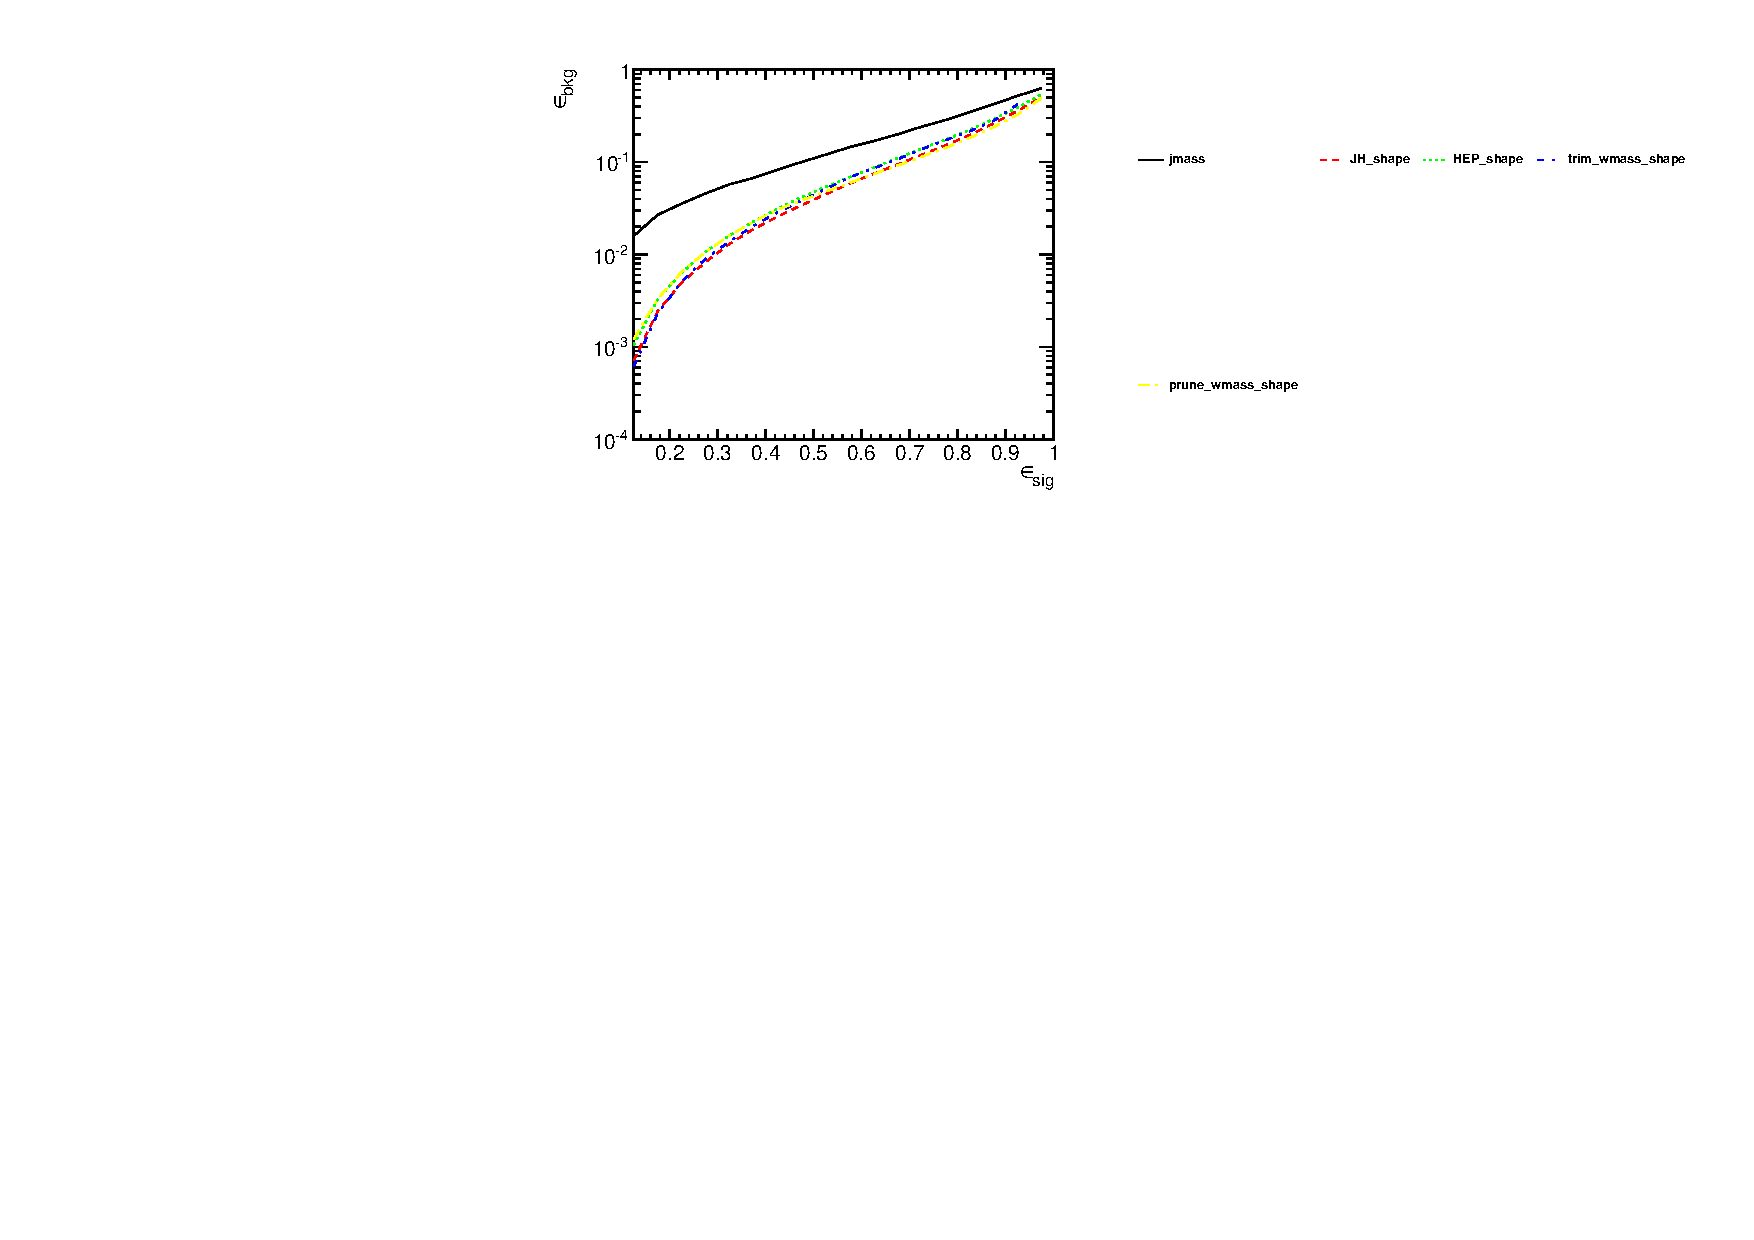
\includegraphics[width=0.48\textwidth]{./Figures/TTagging/0p5TeV_0p8/Rocs_optimum_few.pdf}}
\caption{The BDT combinations in the \pt 500 GeV bin using the anti-\kT R=0.8 algorithm.}
\label{fig:pt500_taggers_AKt_R08}
\end{center}
\end{figure*}

\subsection{Performance at high boost}

\begin{figure*}
\begin{center}
\subfigure[HEPTopTagger]{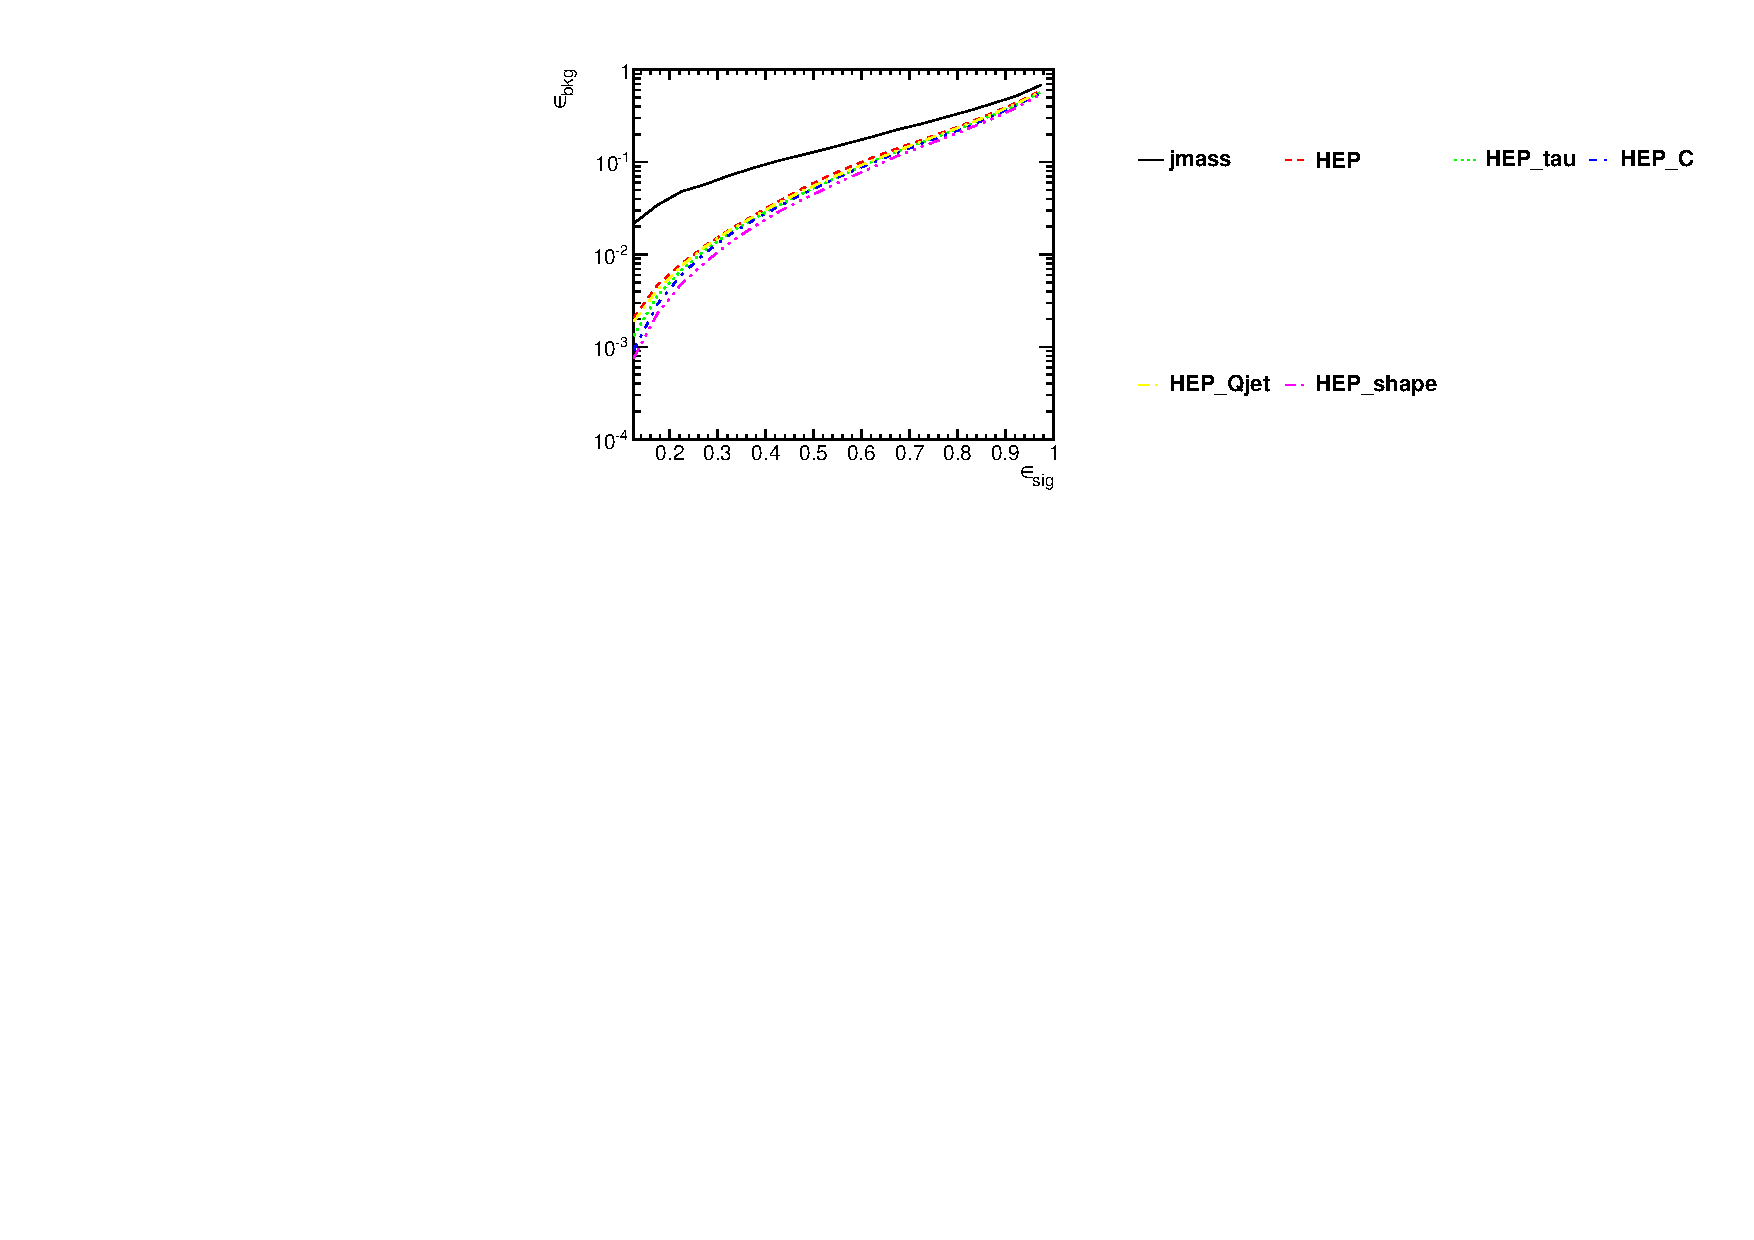
\includegraphics[width=0.48\textwidth]{./Figures/TTagging/1TeV_0p8/Rocs_HEP_few.pdf}}
\subfigure[Johns Hopkins Tagger]{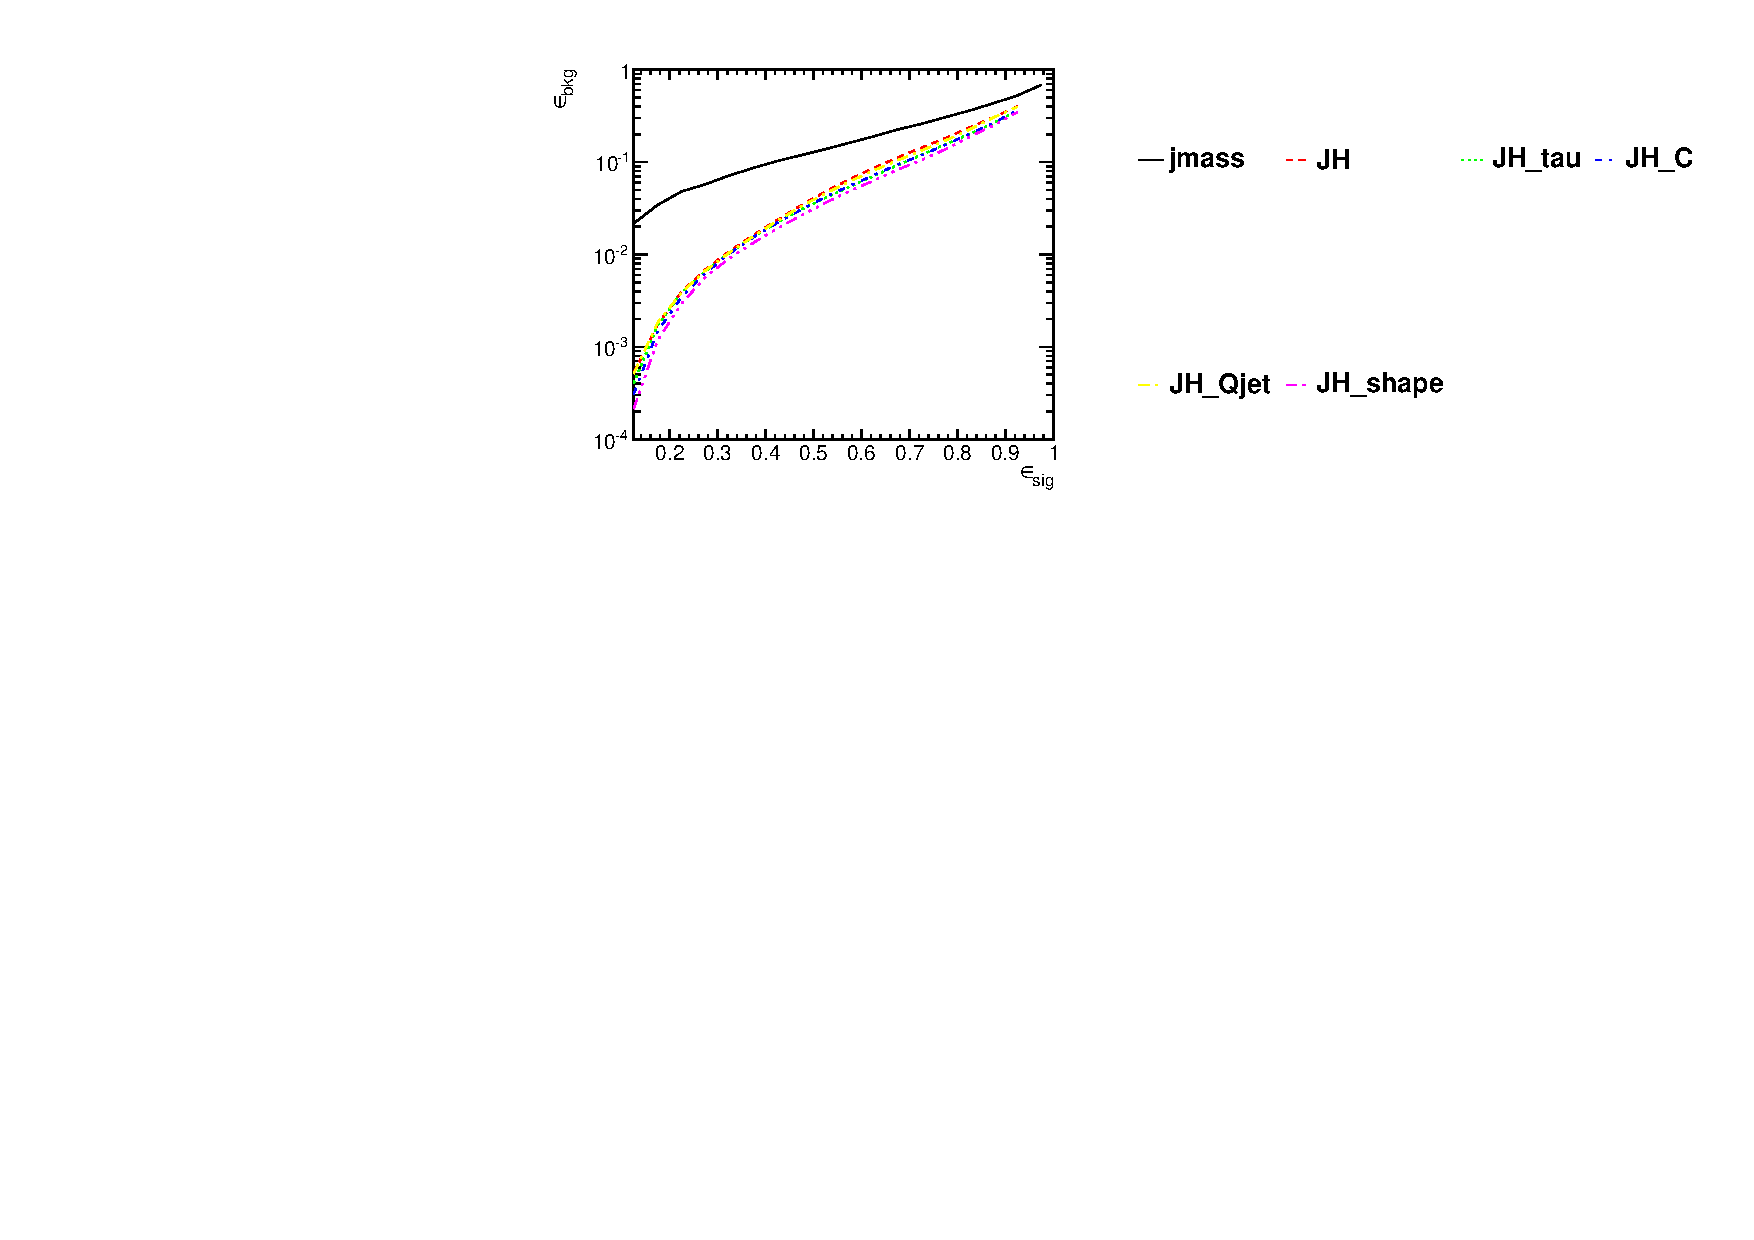
\includegraphics[width=0.48\textwidth]{./Figures/TTagging/1TeV_0p8/Rocs_JH_few.pdf}}
\subfigure[Pruning]{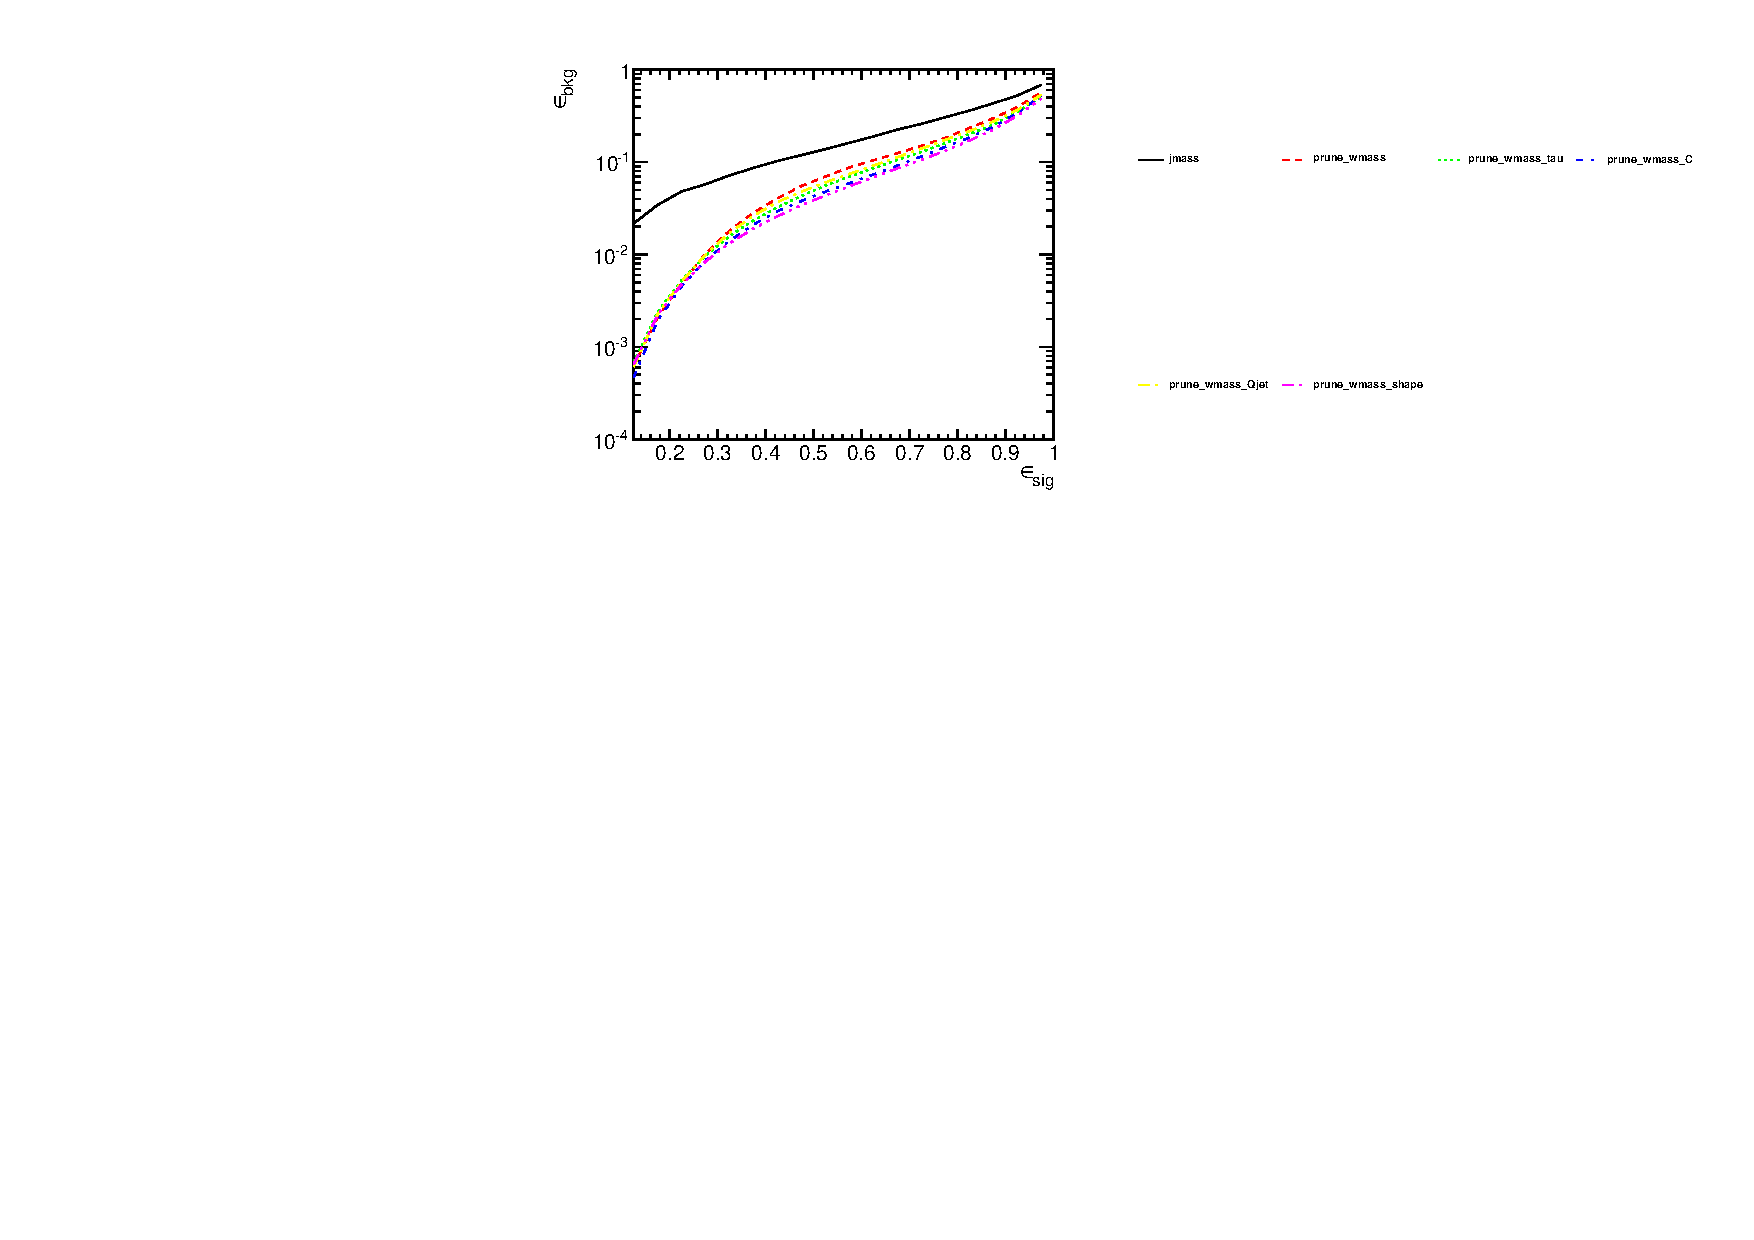
\includegraphics[width=0.48\textwidth]{./Figures/TTagging/1TeV_0p8/Rocs_prune_few.pdf}}
\subfigure[Trimming]{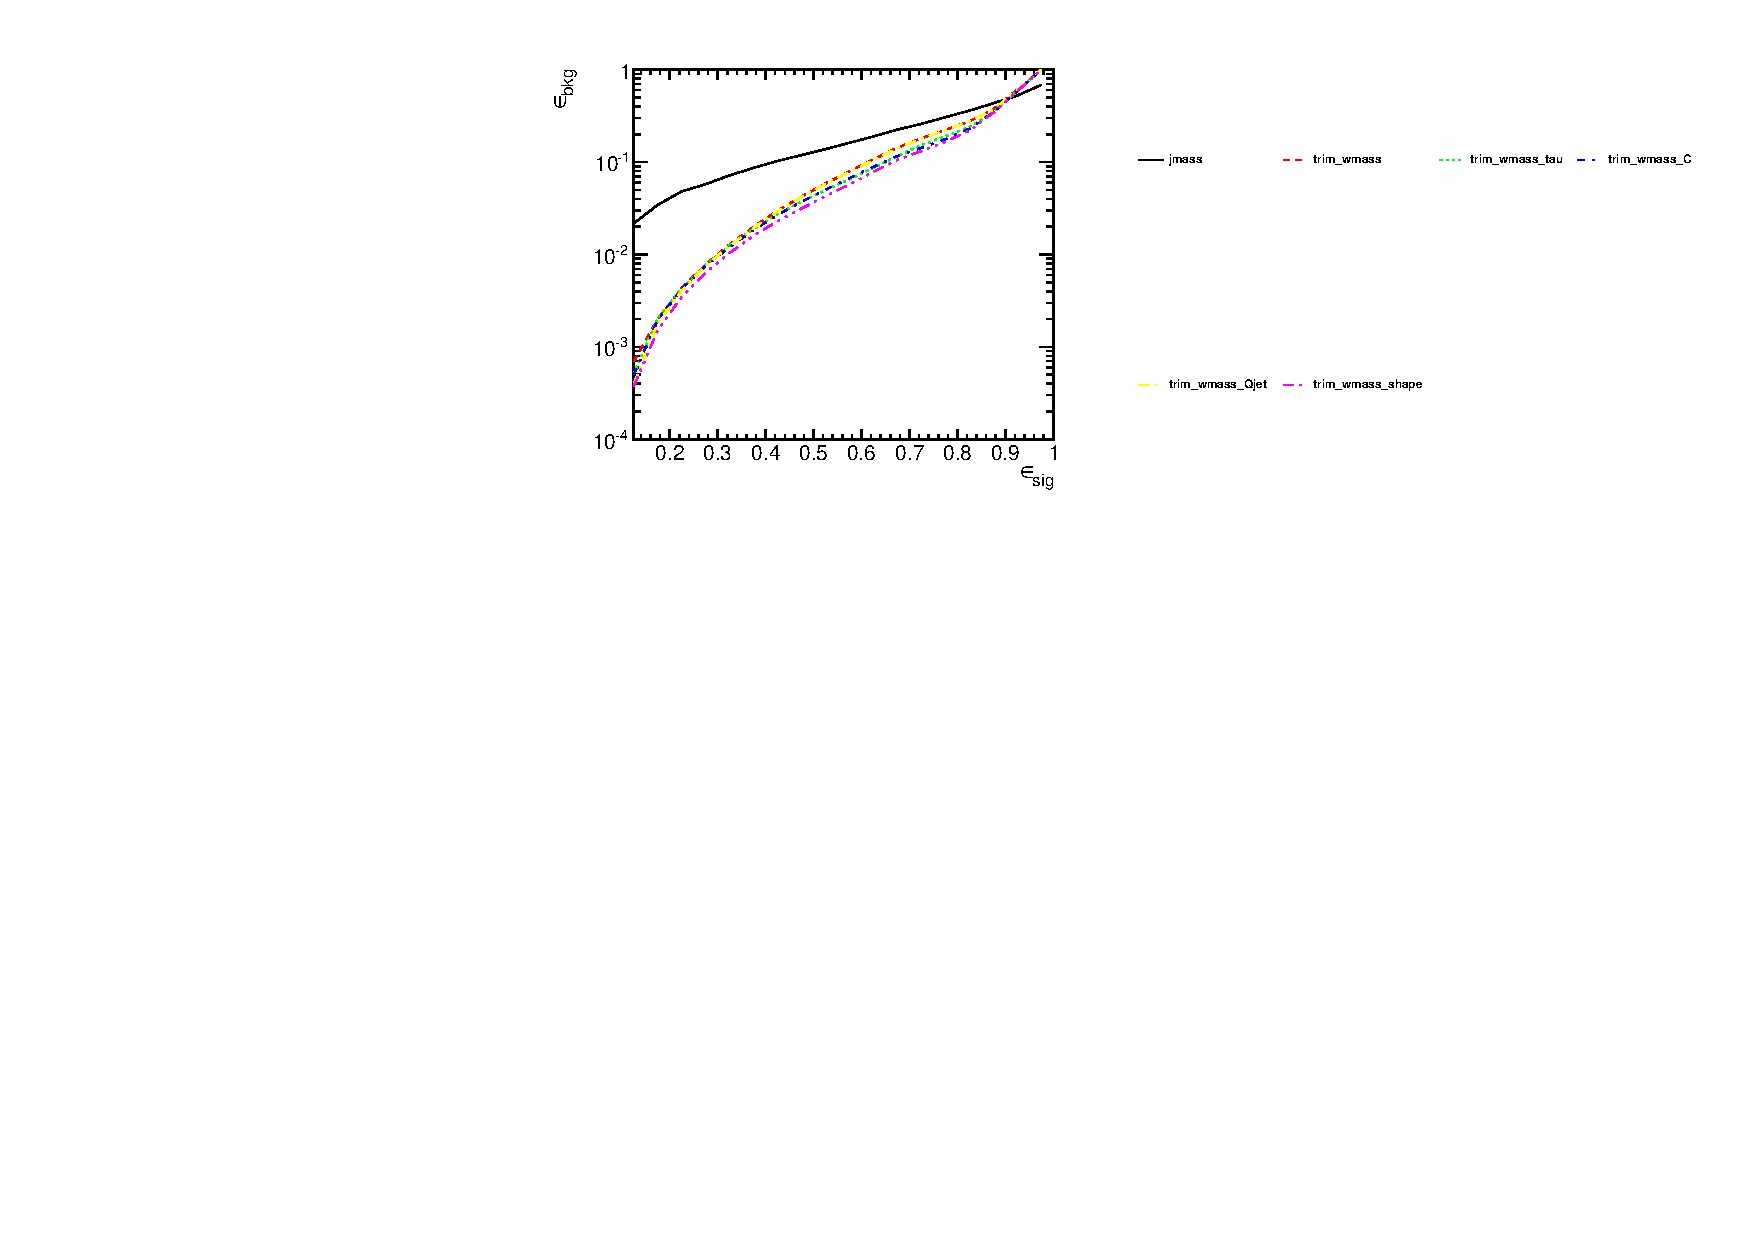
\includegraphics[width=0.48\textwidth]{./Figures/TTagging/1TeV_0p8/Rocs_trim_few.pdf}}
\subfigure[HEP+JH comparison]{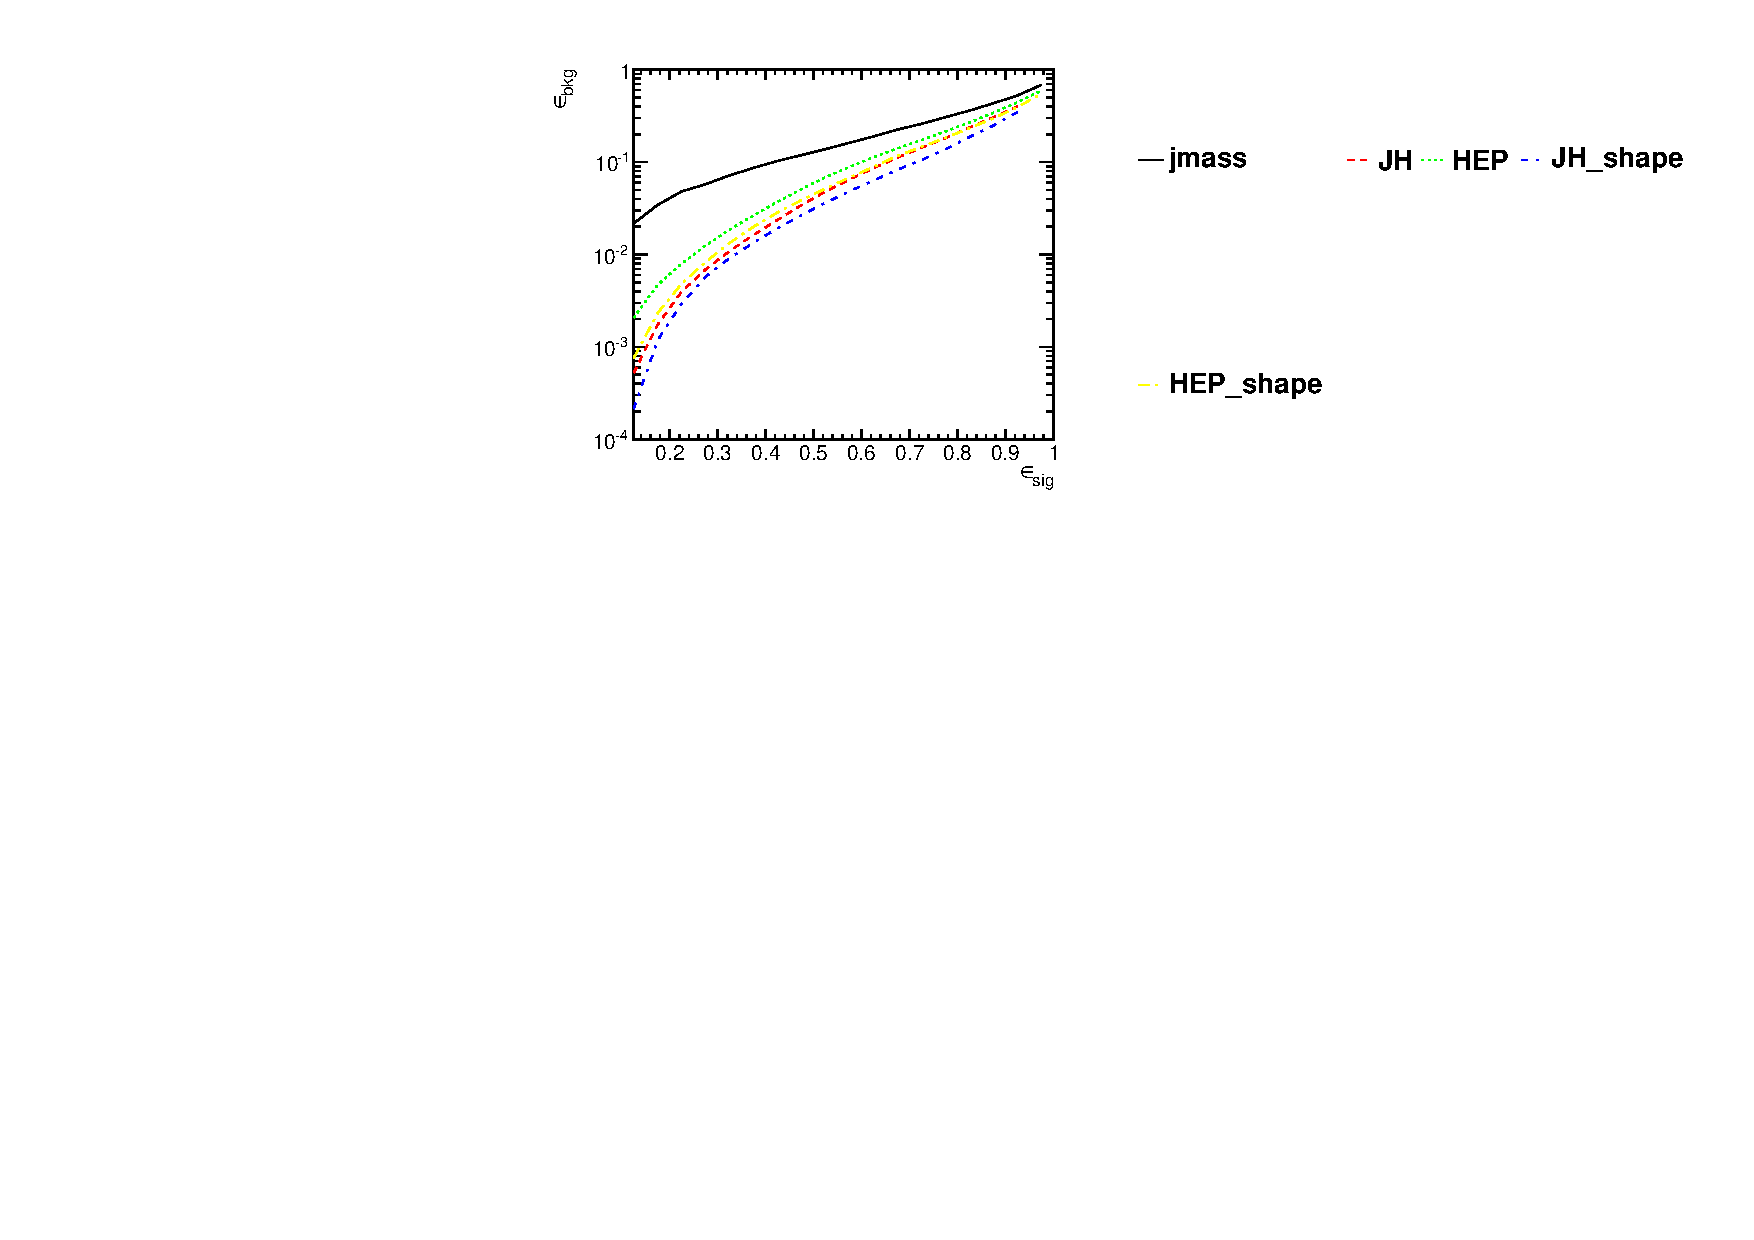
\includegraphics[width=0.48\textwidth]{./Figures/TTagging/1TeV_0p8/Rocs_tagger_shape_few.pdf}}
\subfigure[Grooming comparison]{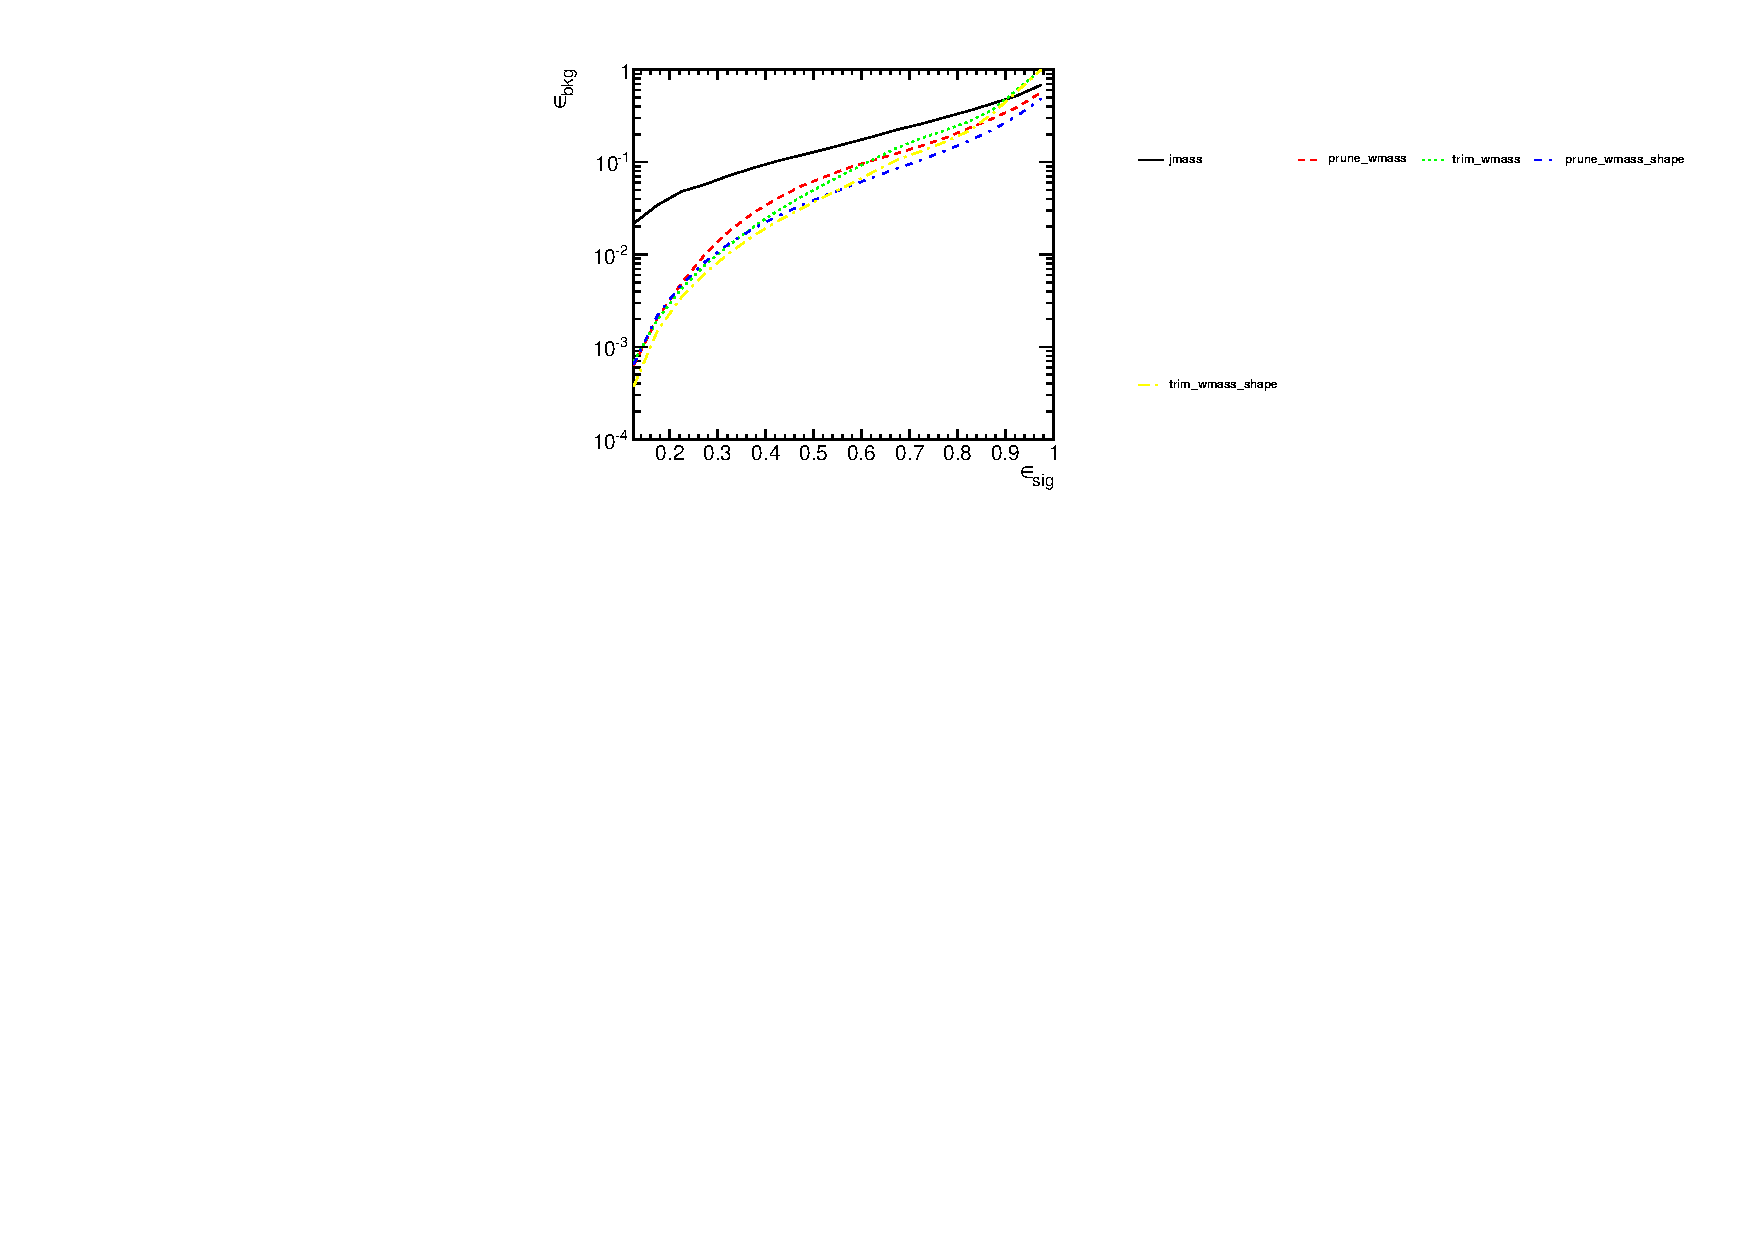
\includegraphics[width=0.48\textwidth]{./Figures/TTagging/1TeV_0p8/Rocs_groom_shape_few.pdf}}
\subfigure[Comparison of Tagger+Shape]{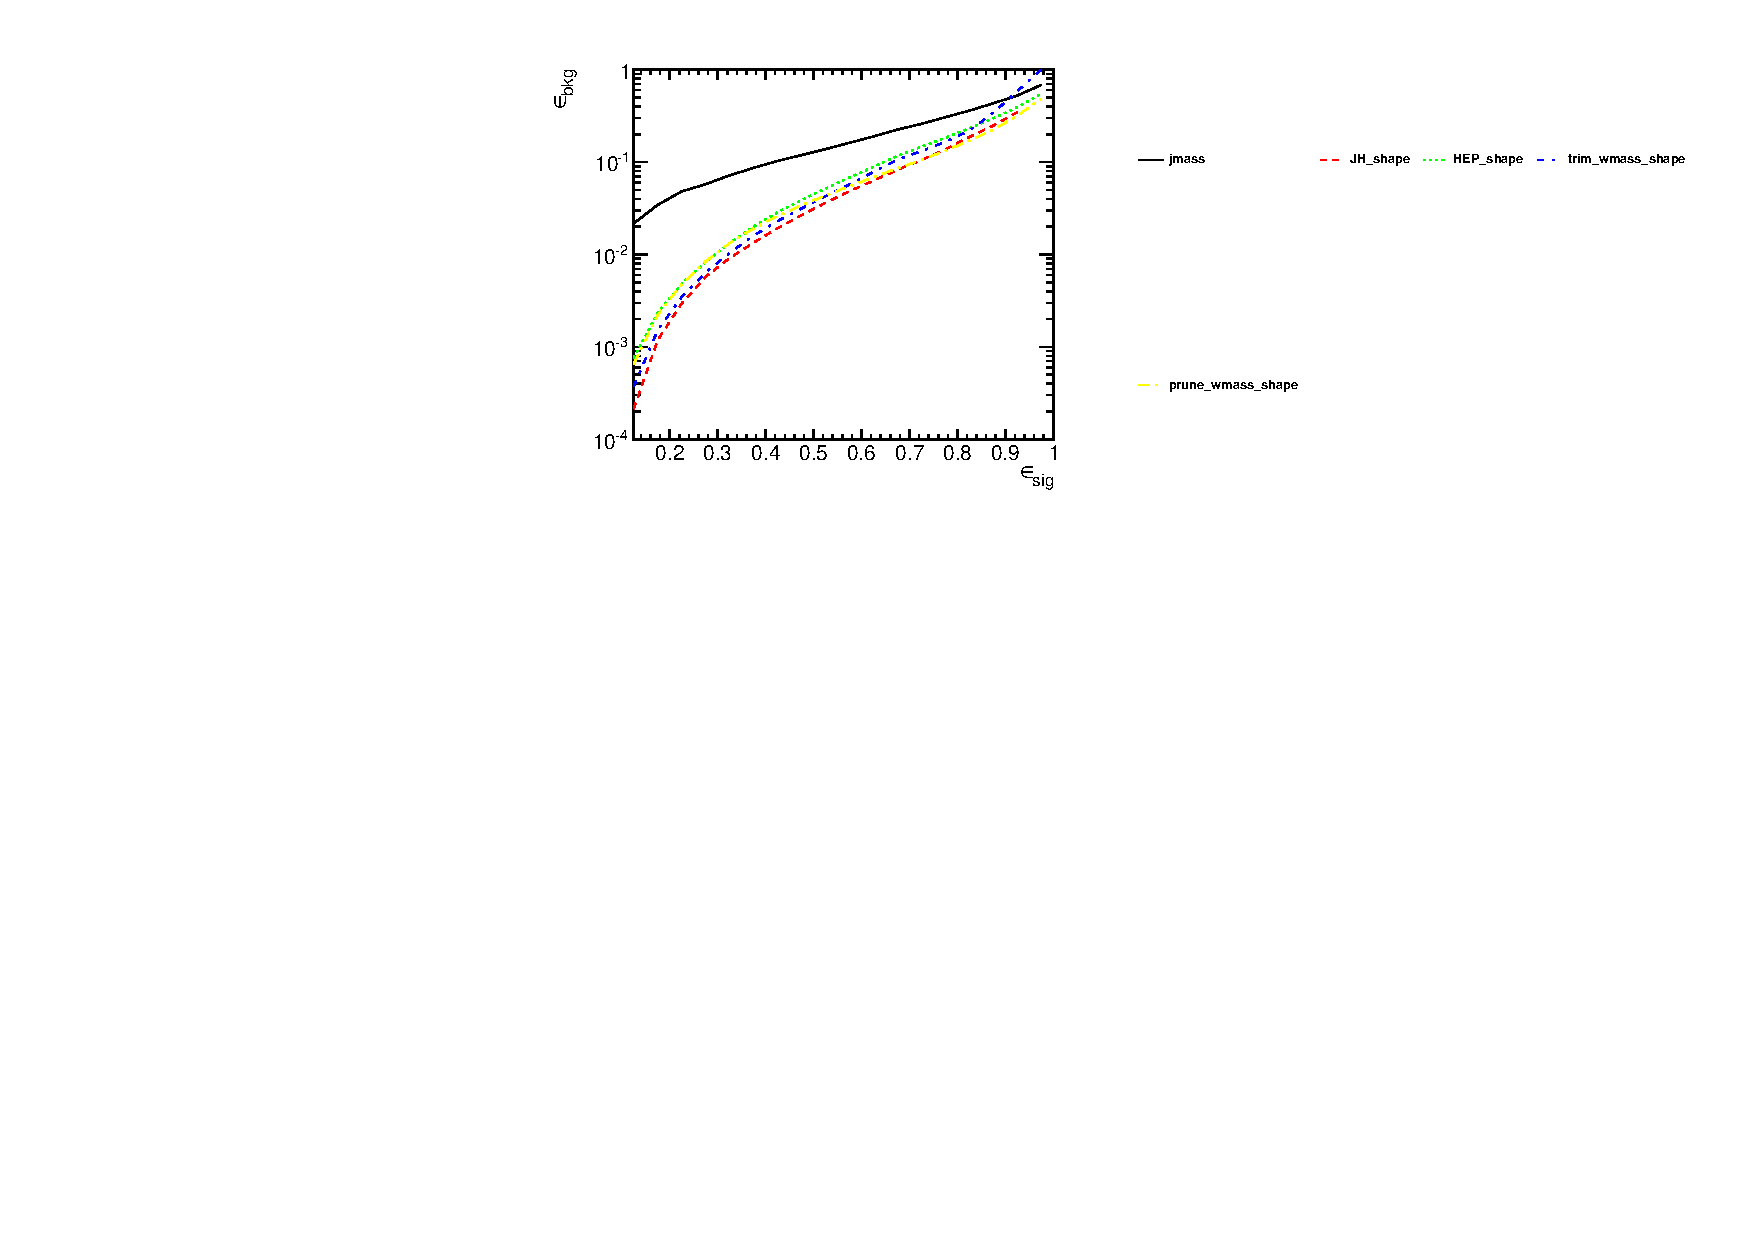
\includegraphics[width=0.48\textwidth]{./Figures/TTagging/1TeV_0p8/Rocs_optimum_few.pdf}}
\caption{The BDT combinations in the \pt 1000 GeV bin using the anti-\kT R=0.8 algorithm.}
\label{fig:pt1000_taggers_AKt_R08}
\end{center}
\end{figure*}

\begin{figure*}
\begin{center}
\subfigure[HEPTopTagger]{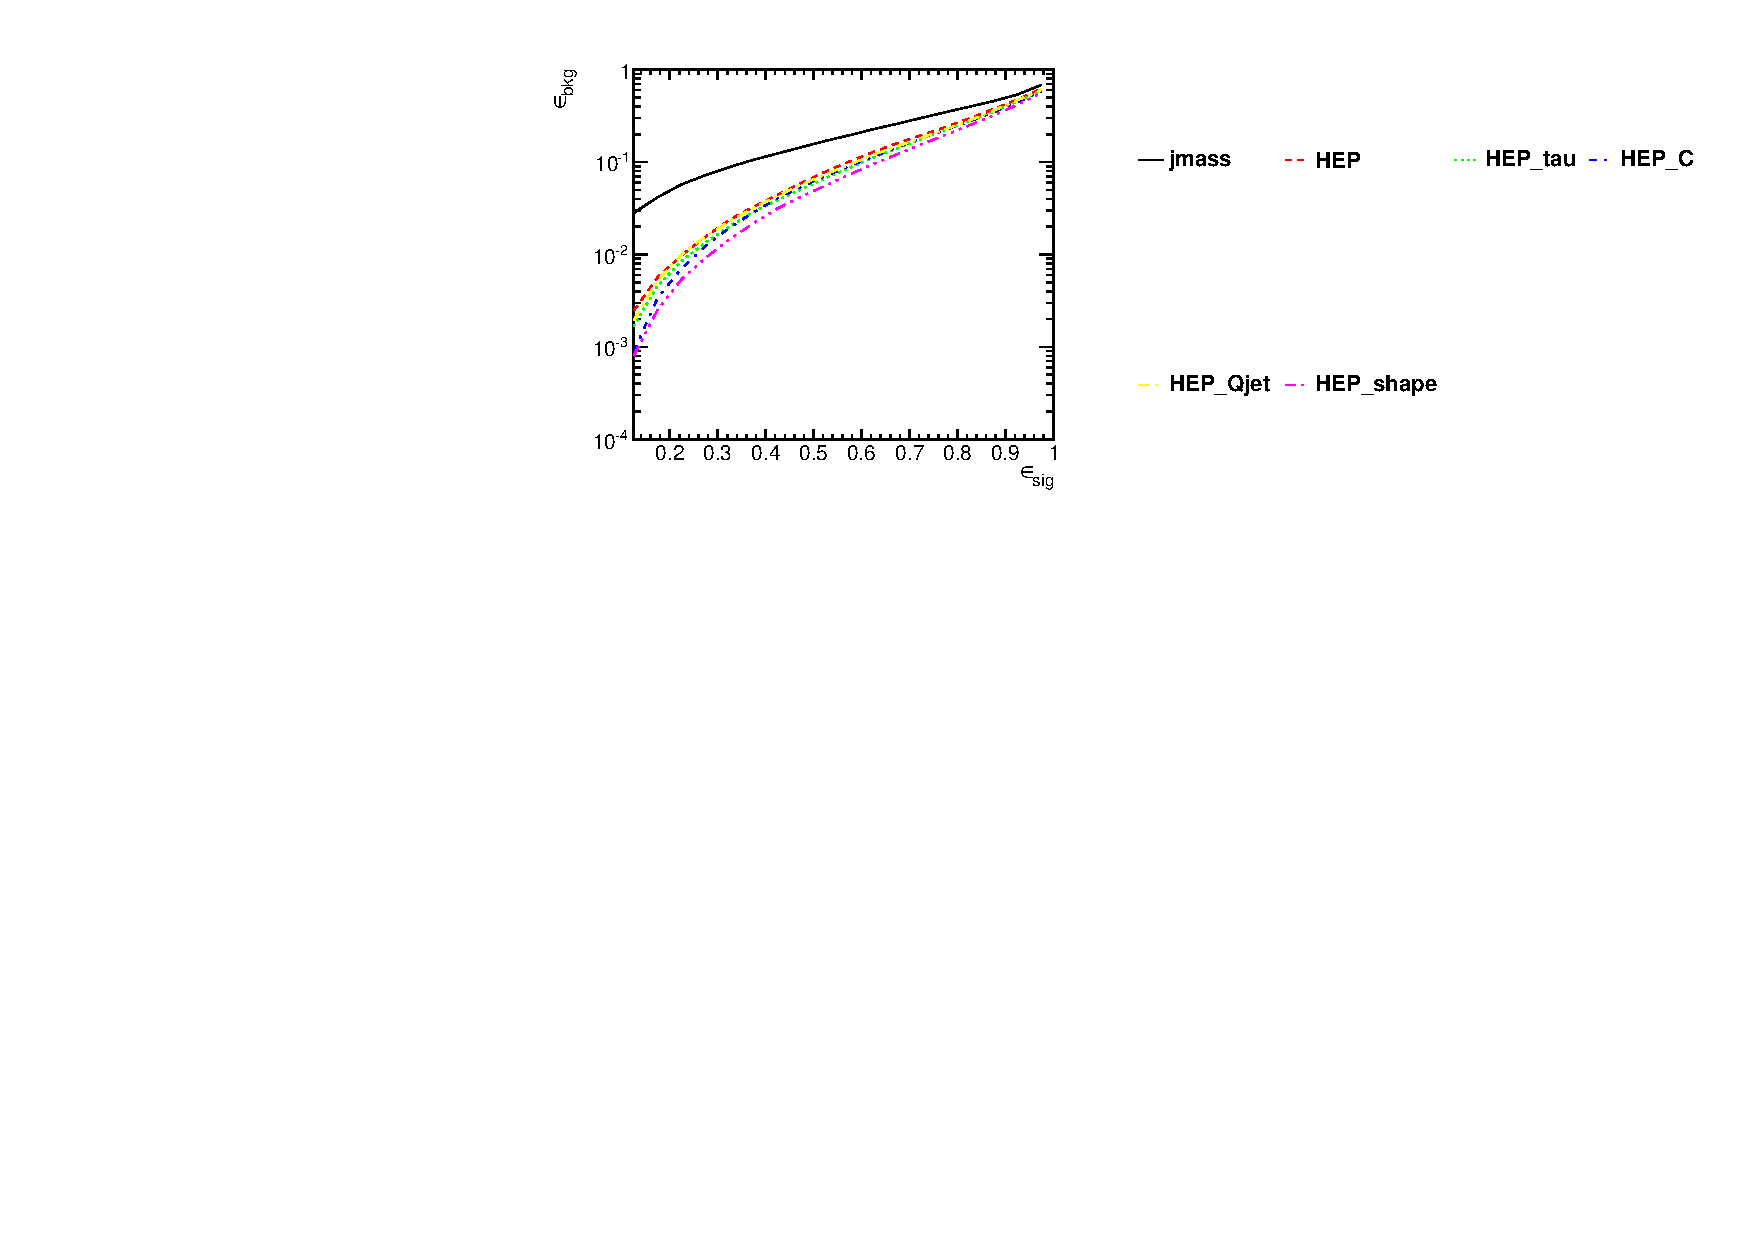
\includegraphics[width=0.48\textwidth]{./Figures/TTagging/1p5TeV_0p8/Rocs_HEP_few.pdf}}
\subfigure[Johns Hopkins Tagger]{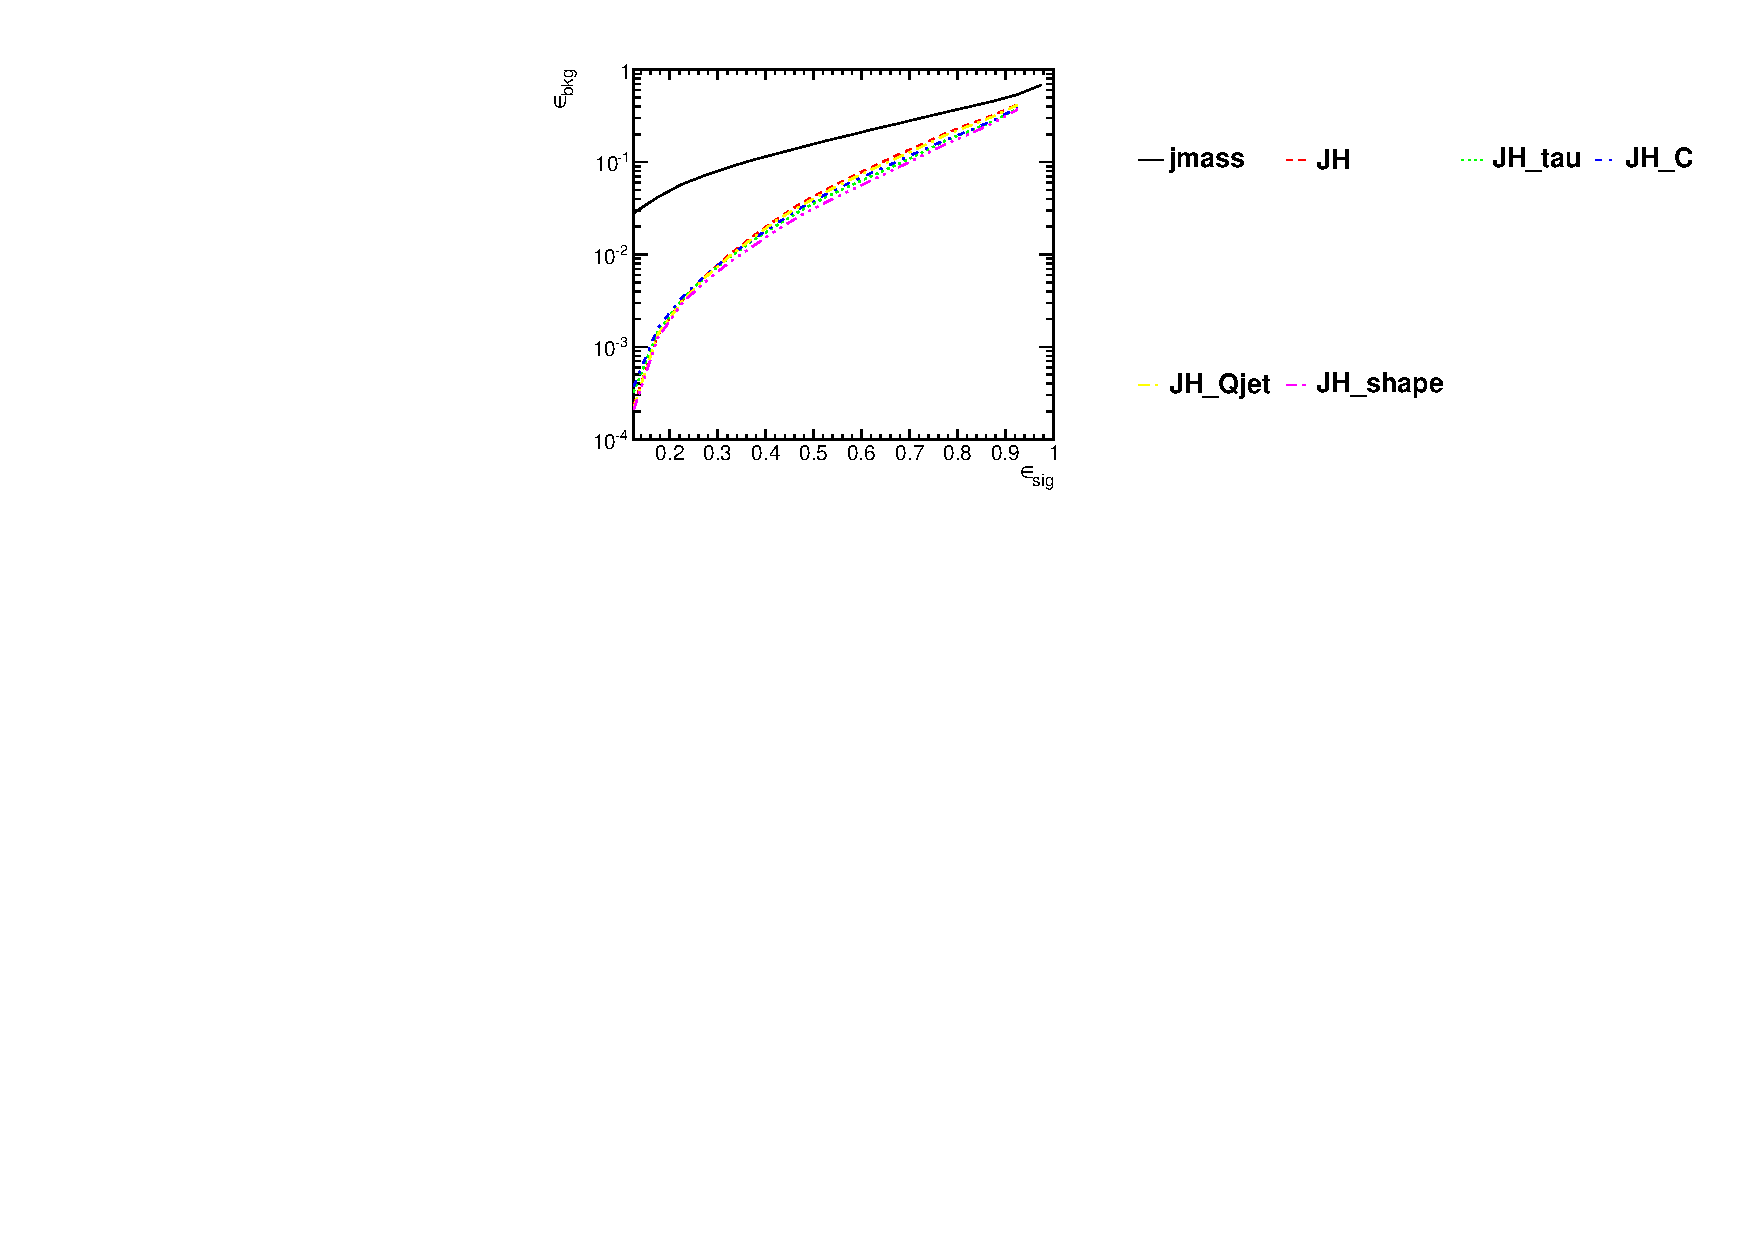
\includegraphics[width=0.48\textwidth]{./Figures/TTagging/1p5TeV_0p8/Rocs_JH_few.pdf}}
\subfigure[Pruning]{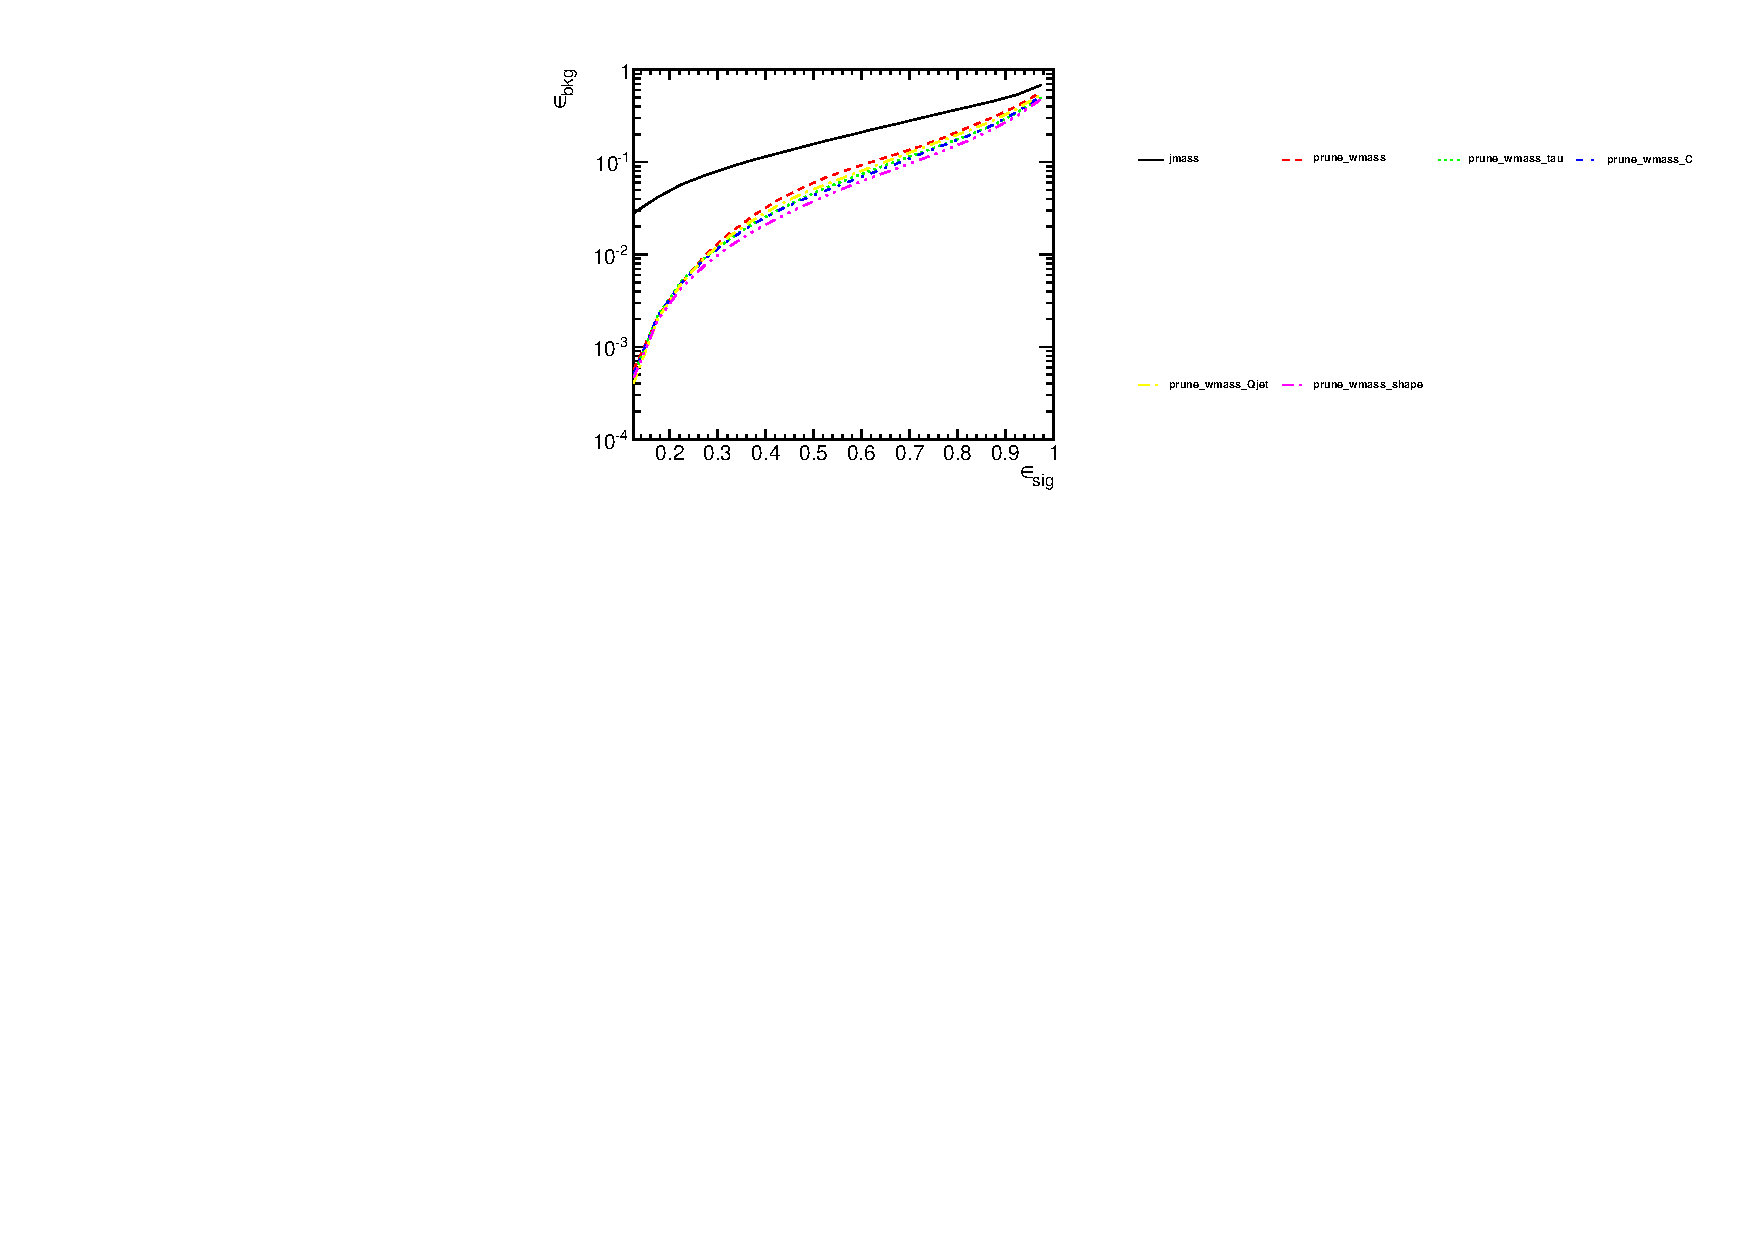
\includegraphics[width=0.48\textwidth]{./Figures/TTagging/1p5TeV_0p8/Rocs_prune_few.pdf}}
\subfigure[Trimming]{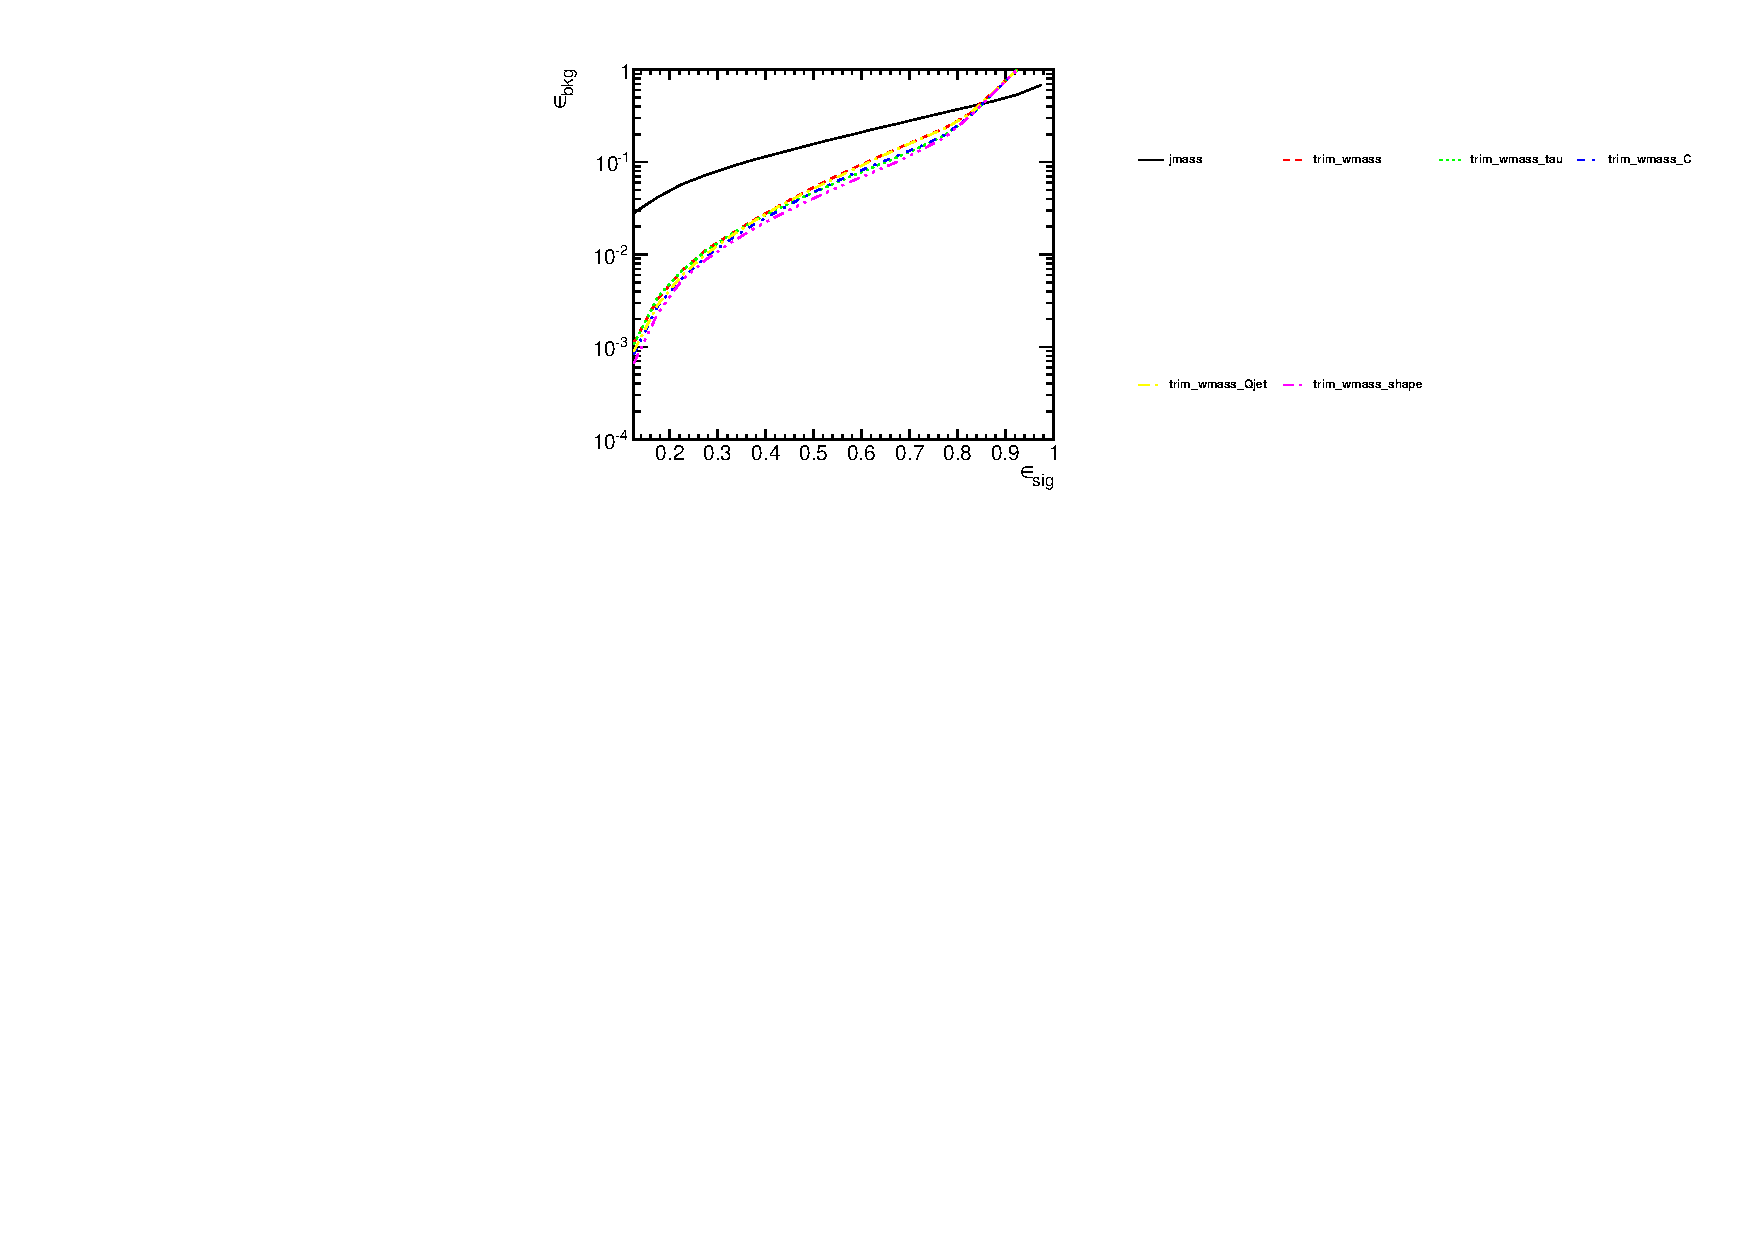
\includegraphics[width=0.48\textwidth]{./Figures/TTagging/1p5TeV_0p8/Rocs_trim_few.pdf}}
\subfigure[HEP+JH comparison]{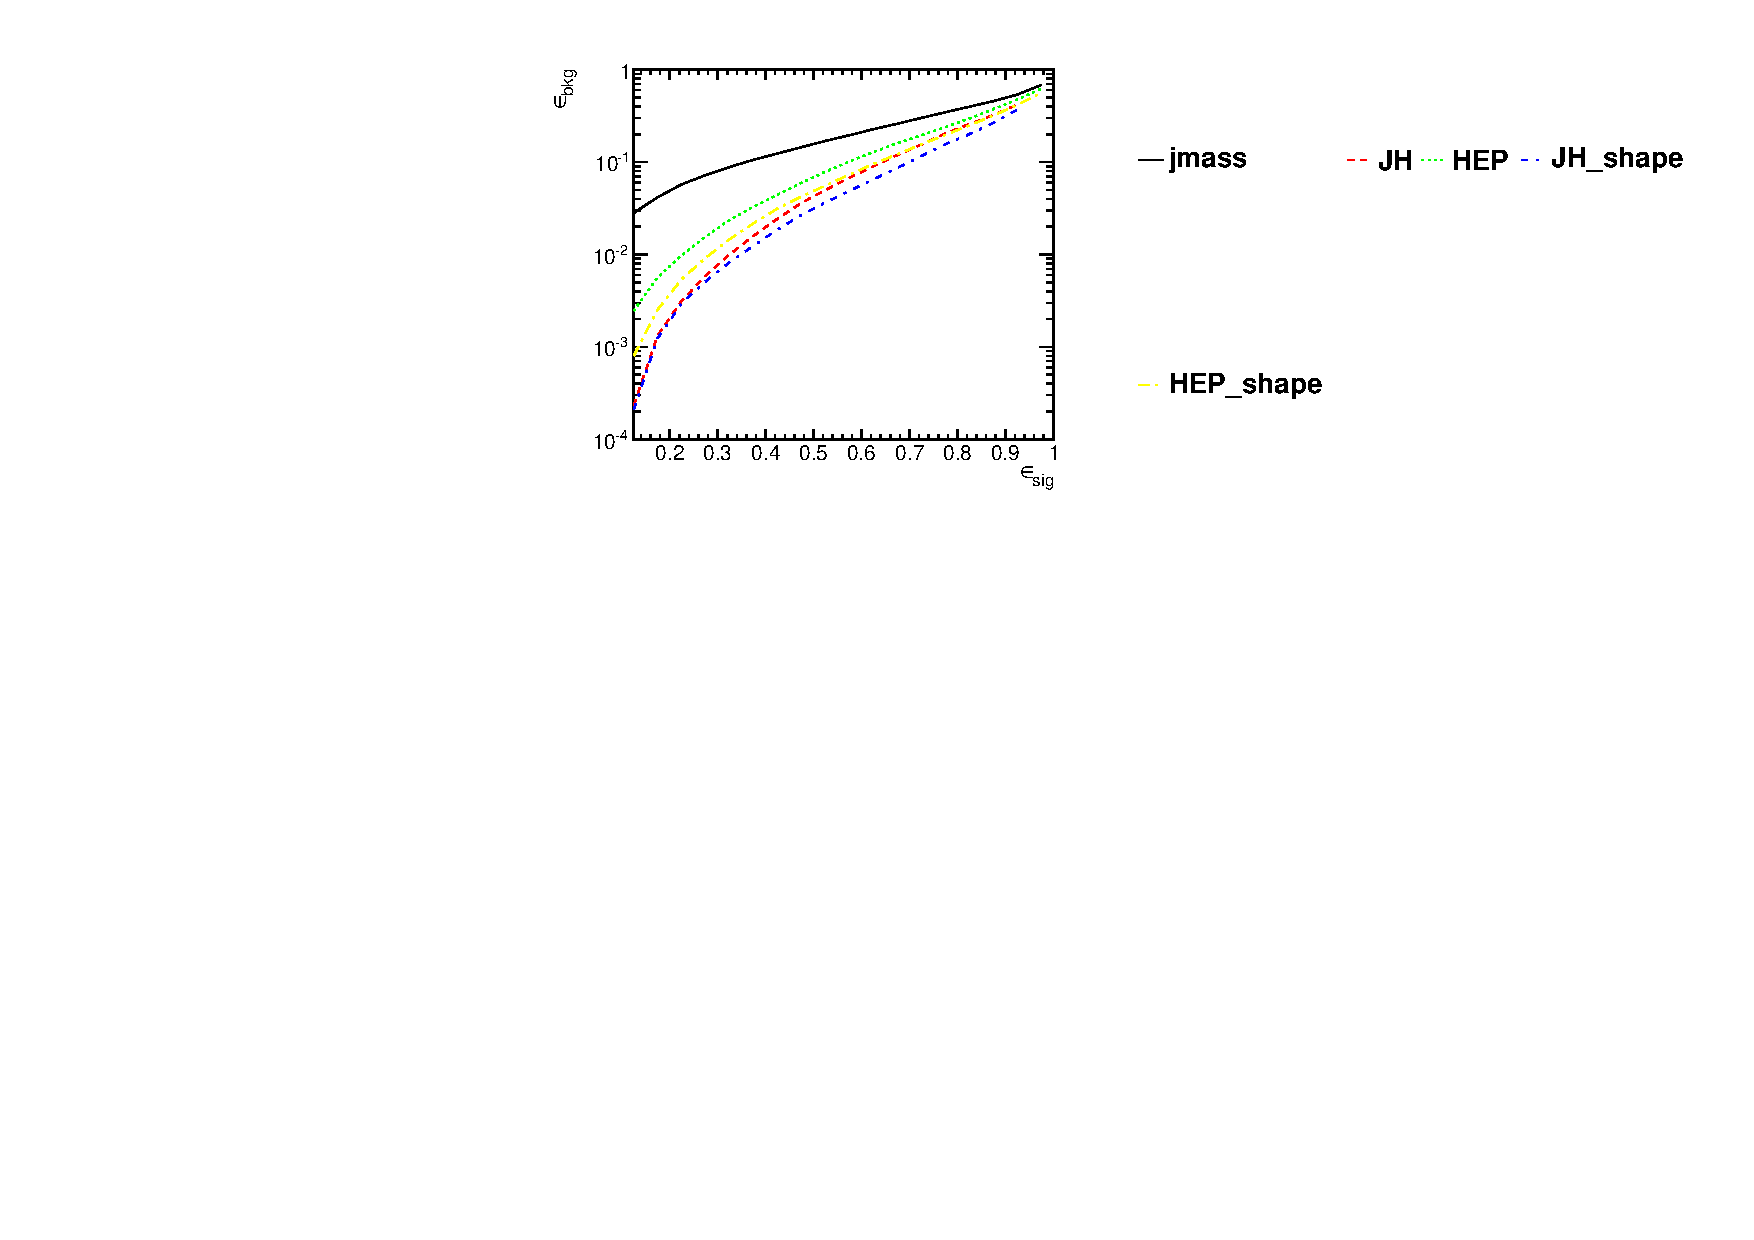
\includegraphics[width=0.48\textwidth]{./Figures/TTagging/1p5TeV_0p8/Rocs_tagger_shape_few.pdf}}
\subfigure[Grooming comparison]{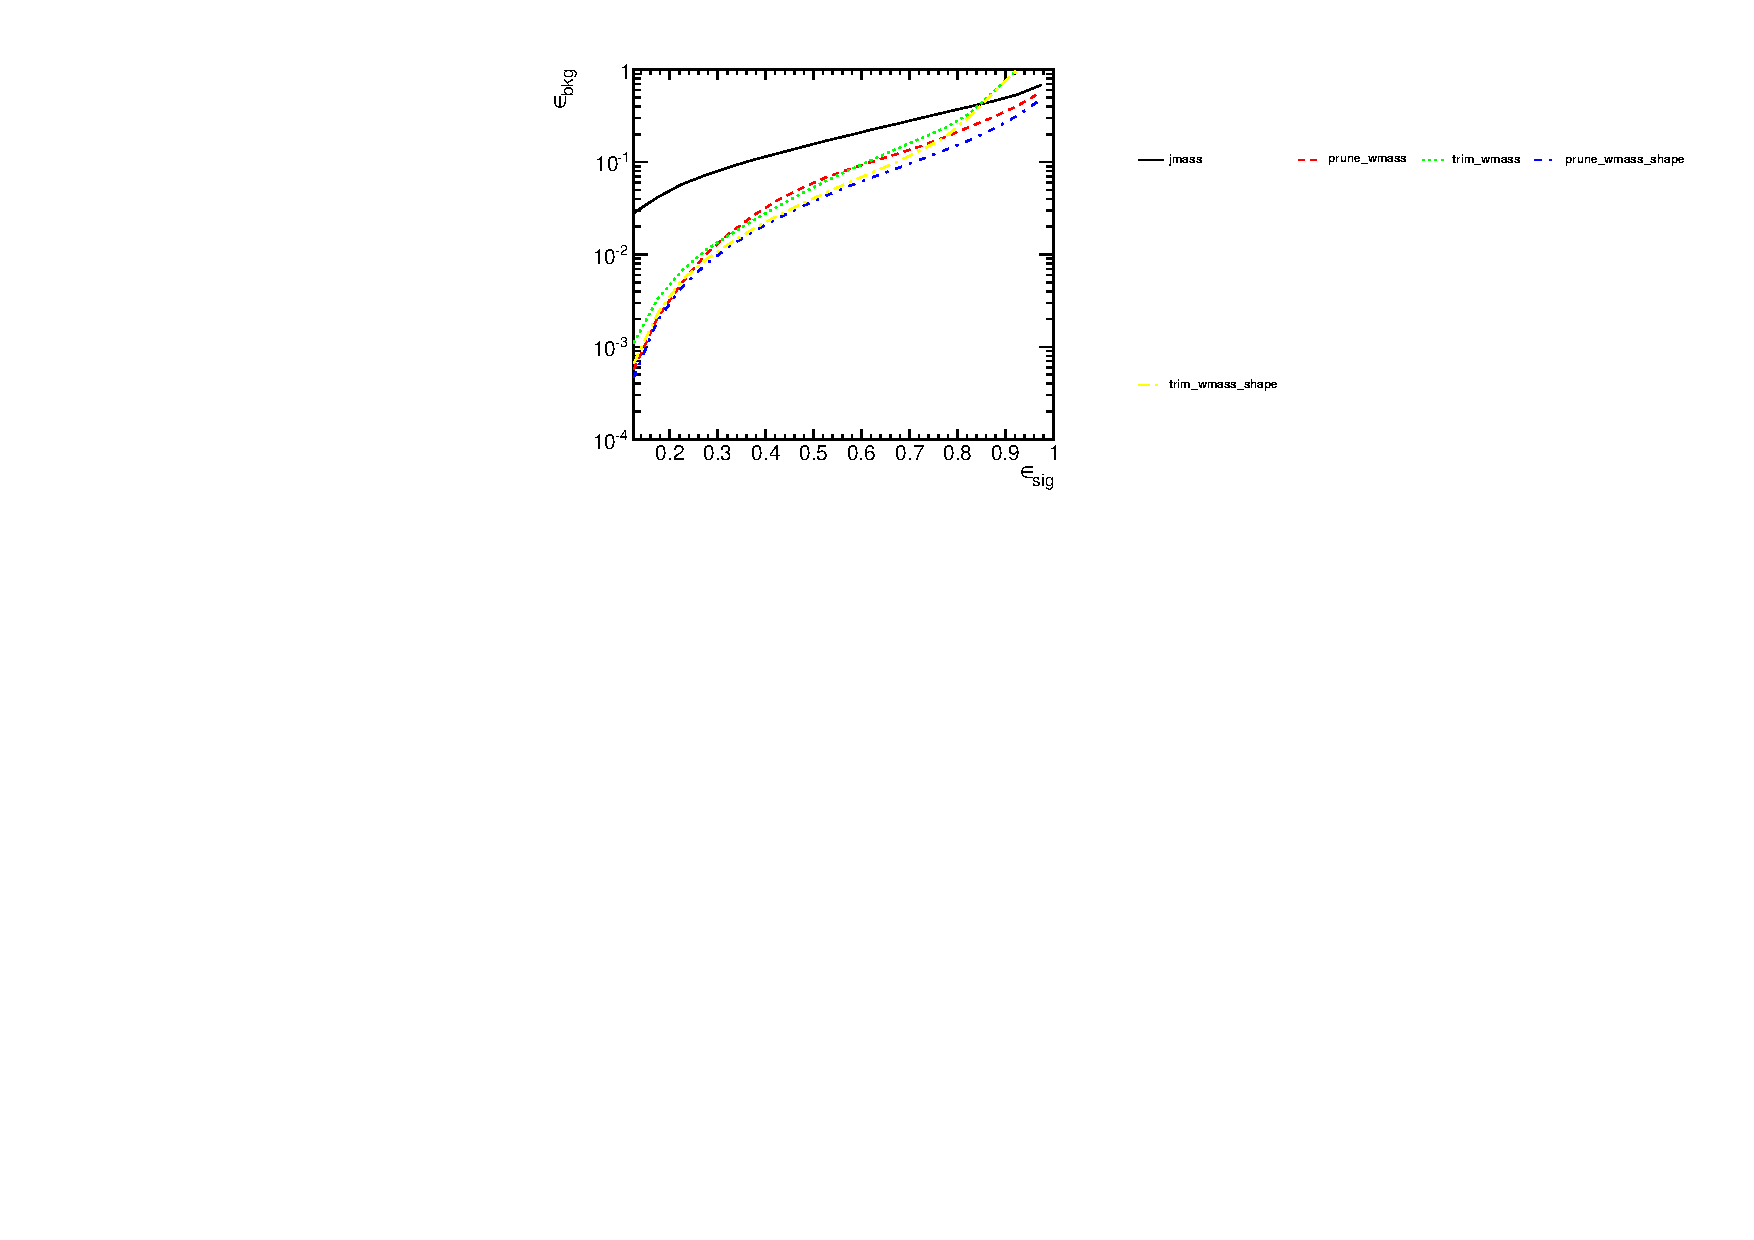
\includegraphics[width=0.48\textwidth]{./Figures/TTagging/1p5TeV_0p8/Rocs_groom_shape_few.pdf}}
\subfigure[Comparison of Tagger+Shape]{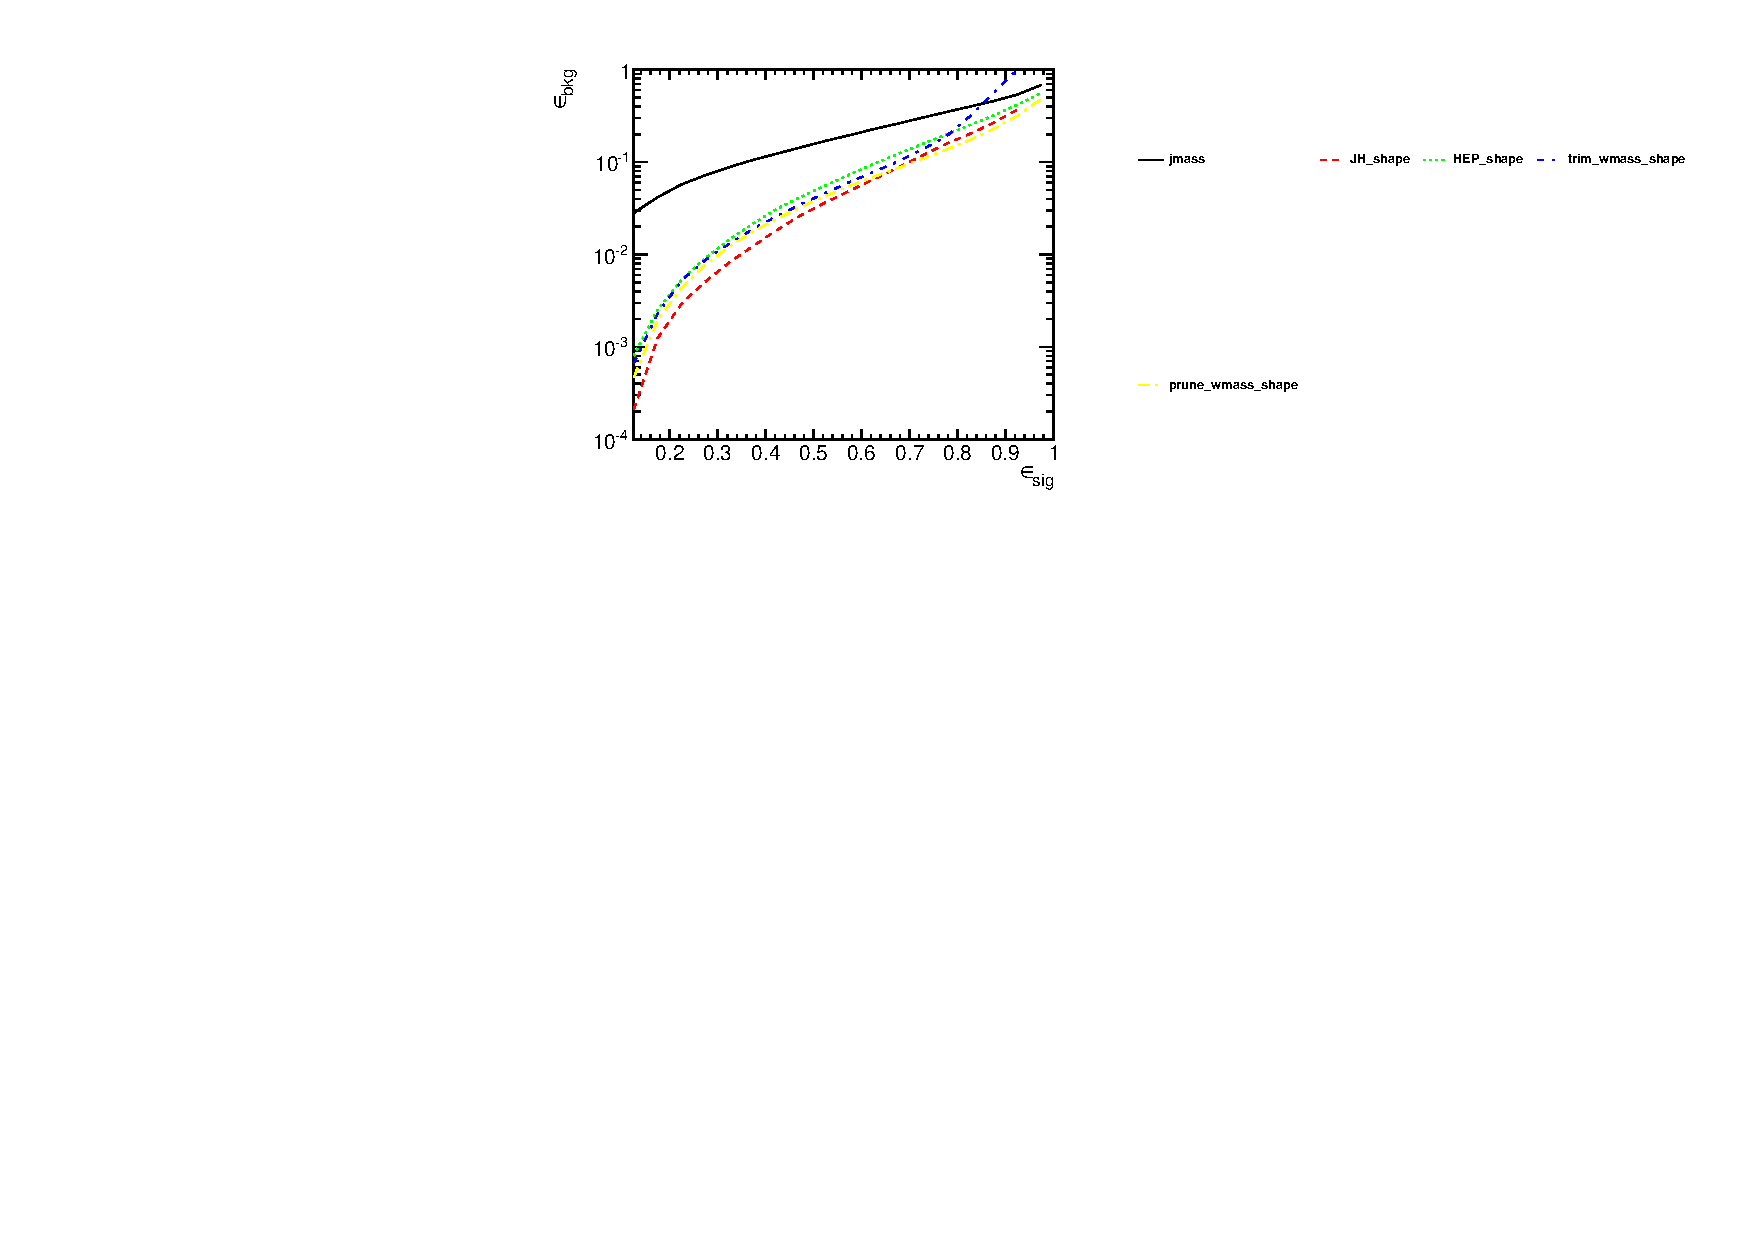
\includegraphics[width=0.48\textwidth]{./Figures/TTagging/1p5TeV_0p8/Rocs_optimum_few.pdf}}
\caption{The BDT combinations in the \pt 1500 GeV bin using the anti-\kT R=0.8 algorithm.}
\label{fig:pt1500_taggers_AKt_R08}
\end{center}
\end{figure*}

\subsection{Direct comparison at different boost}
\begin{figure*}
\begin{center}
\subfigure[C2]{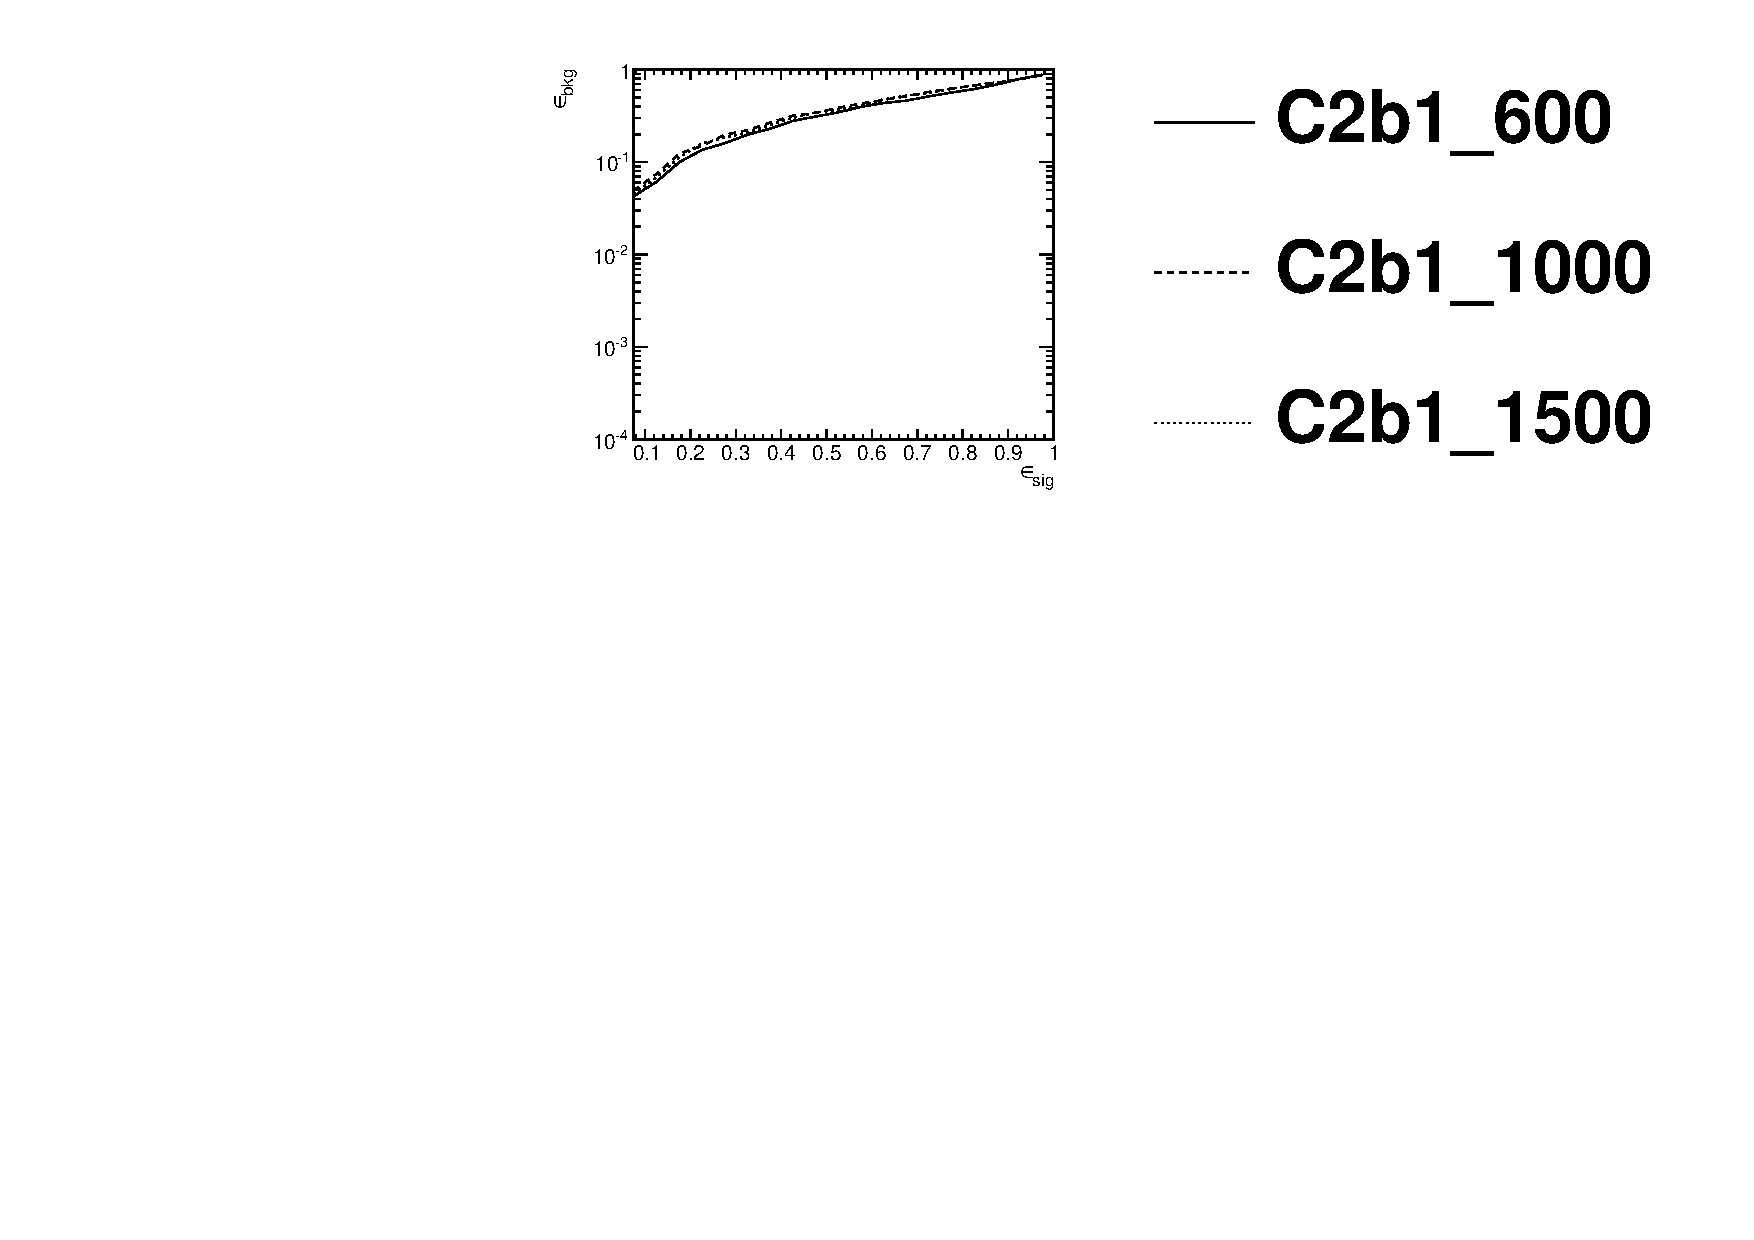
\includegraphics[width=0.48\textwidth]{./Figures/TTagging/pT_compare/Rocs_C2b1_pTcompare.pdf}}
\subfigure[C3]{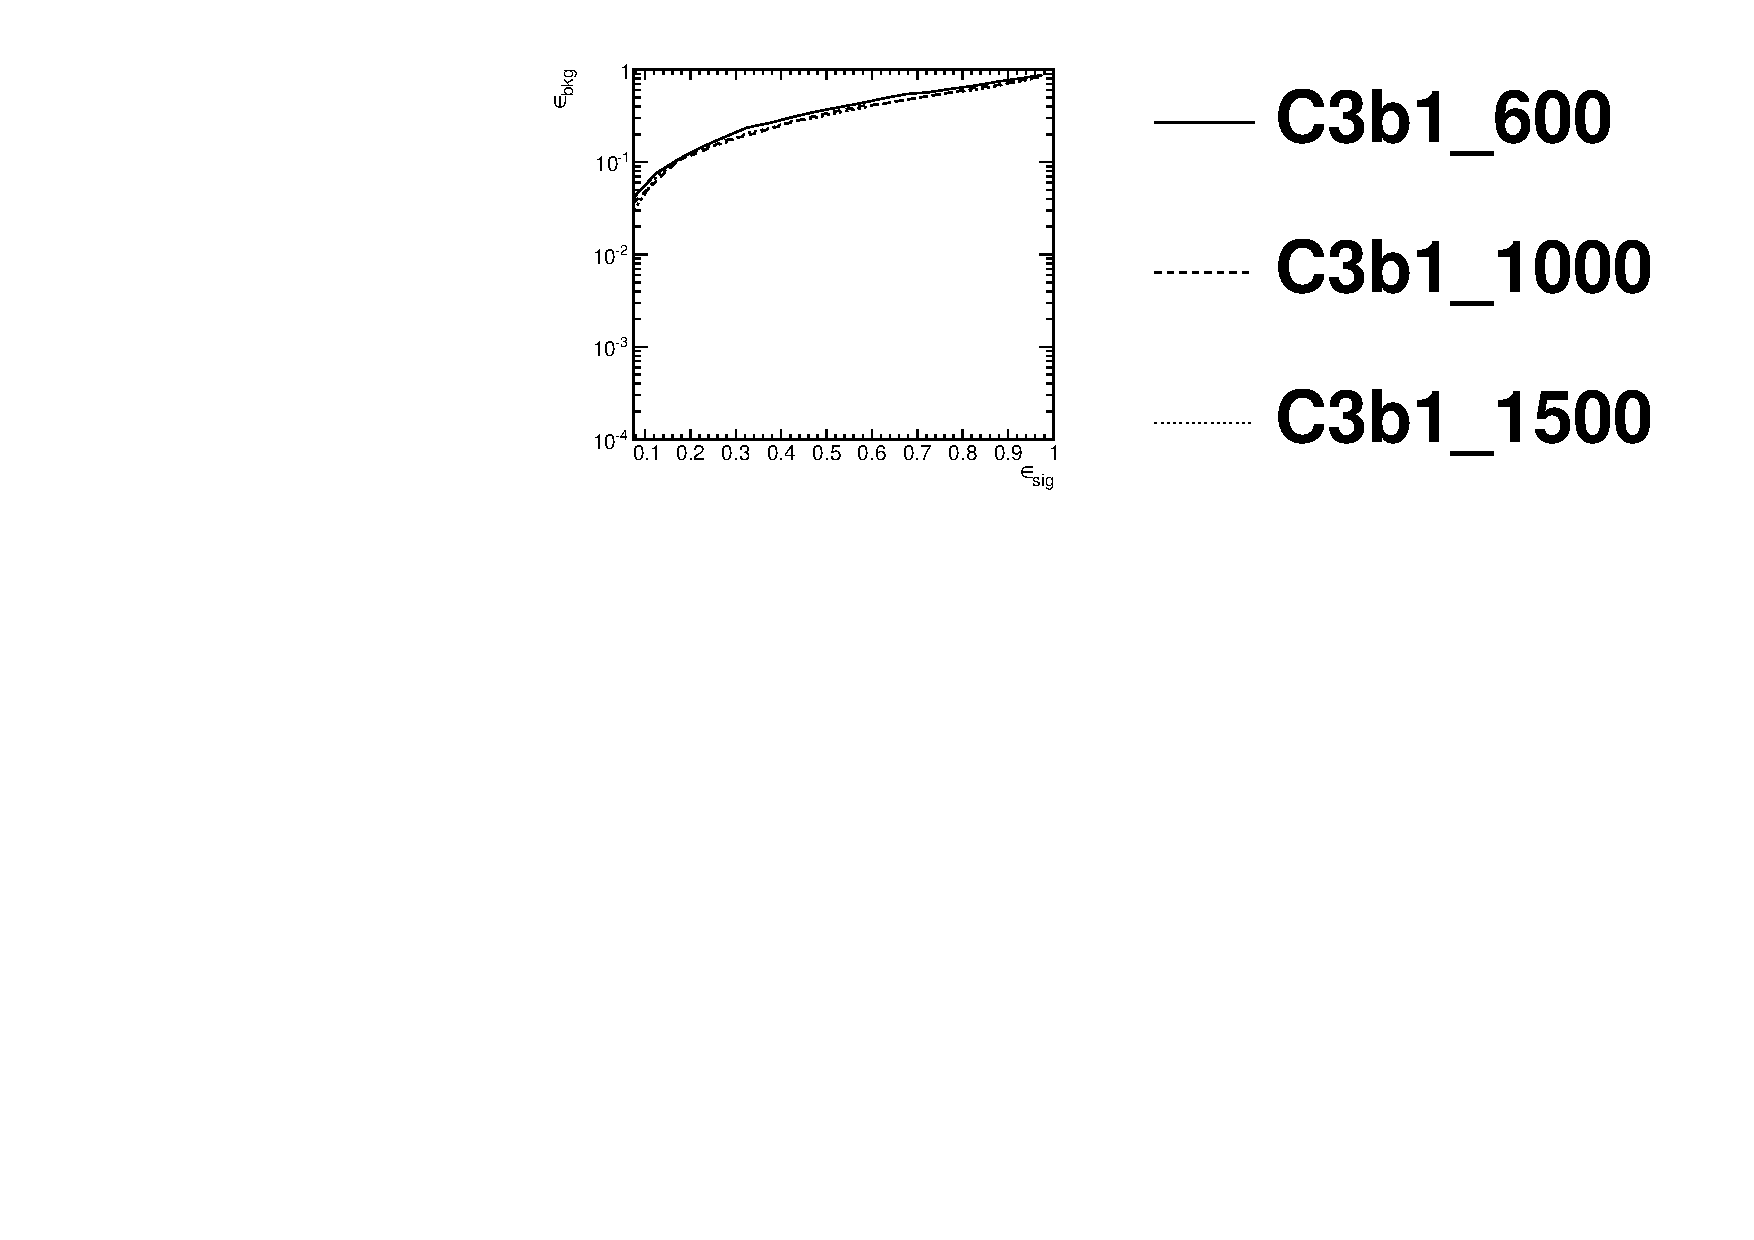
\includegraphics[width=0.48\textwidth]{./Figures/TTagging/pT_compare/Rocs_C3b1_pTcompare.pdf}}
\subfigure[$\tau_{21}$]{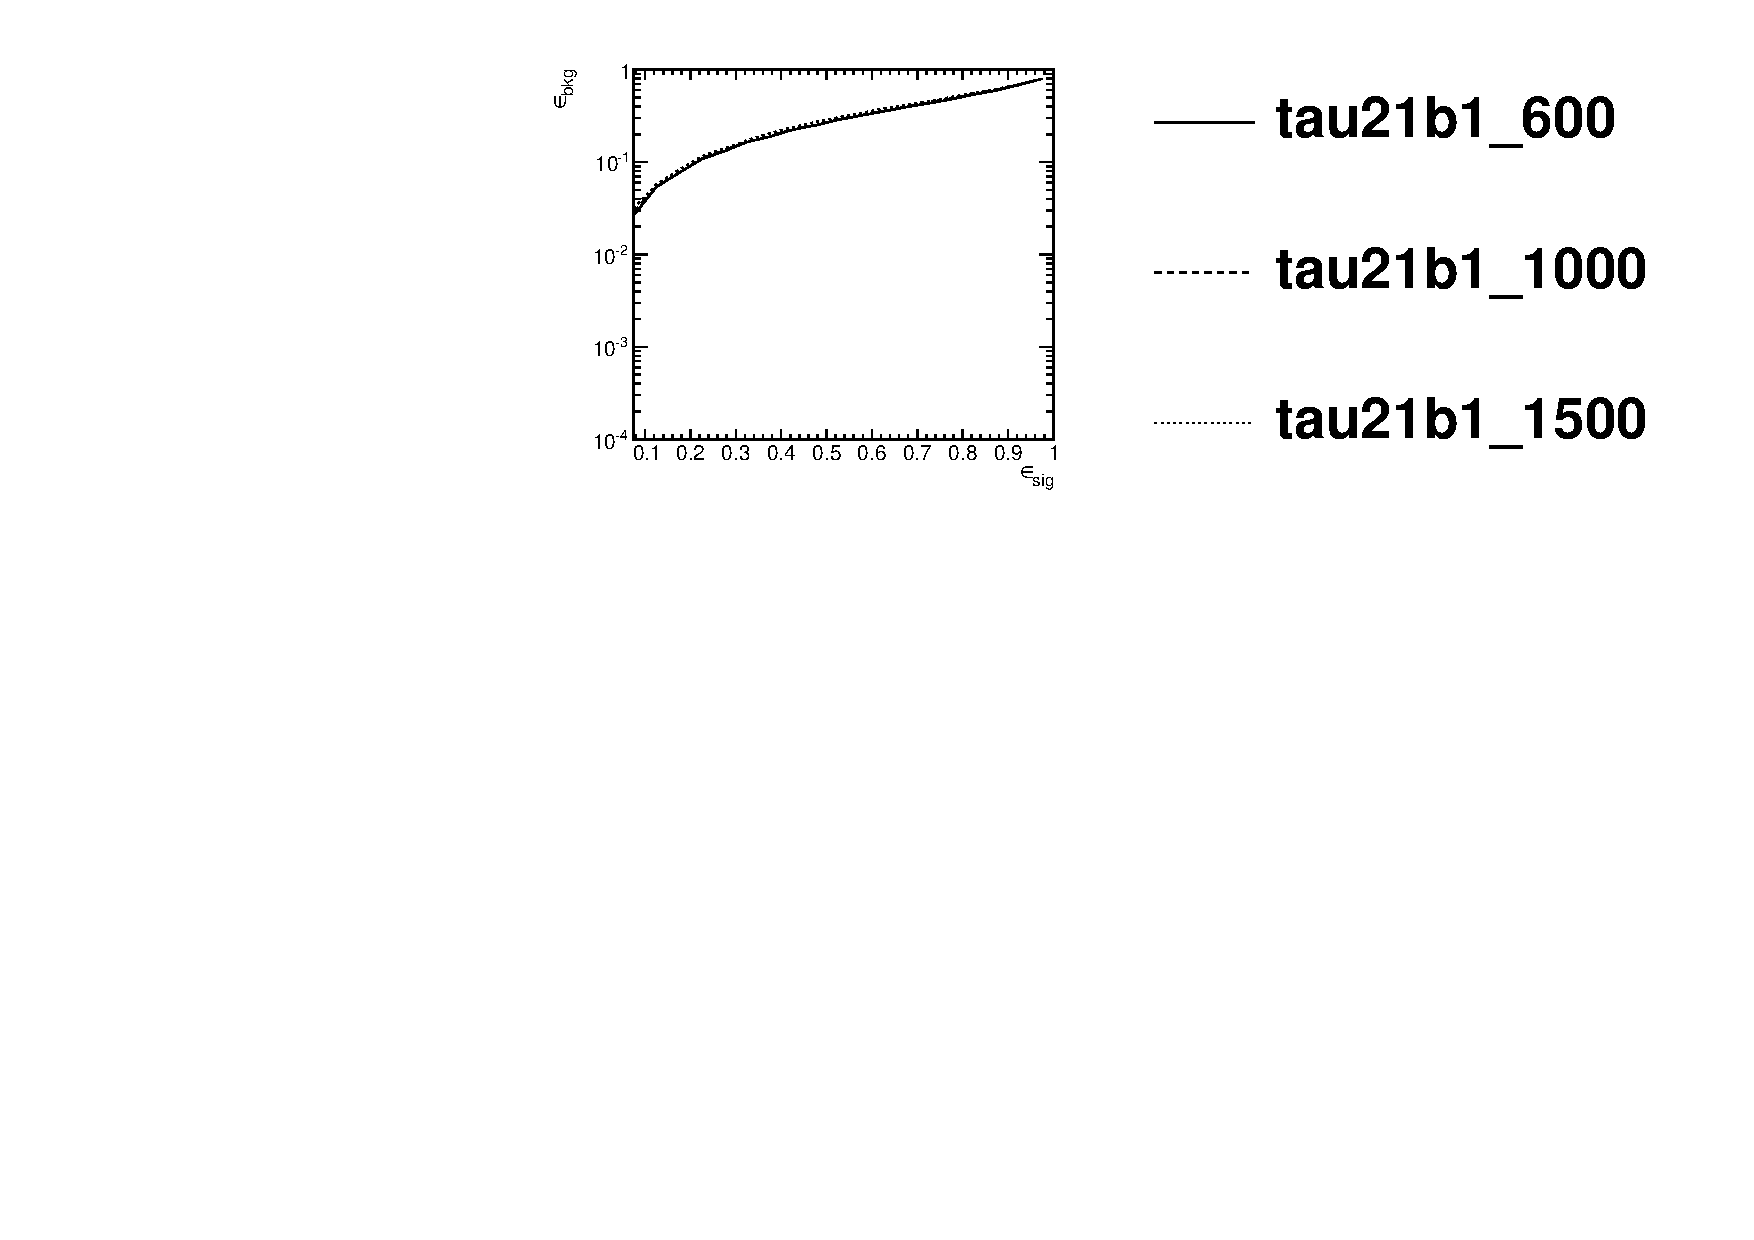
\includegraphics[width=0.48\textwidth]{./Figures/TTagging/pT_compare/Rocs_tau21b1_pTcompare.pdf}}
\subfigure[$\tau_{32}$]{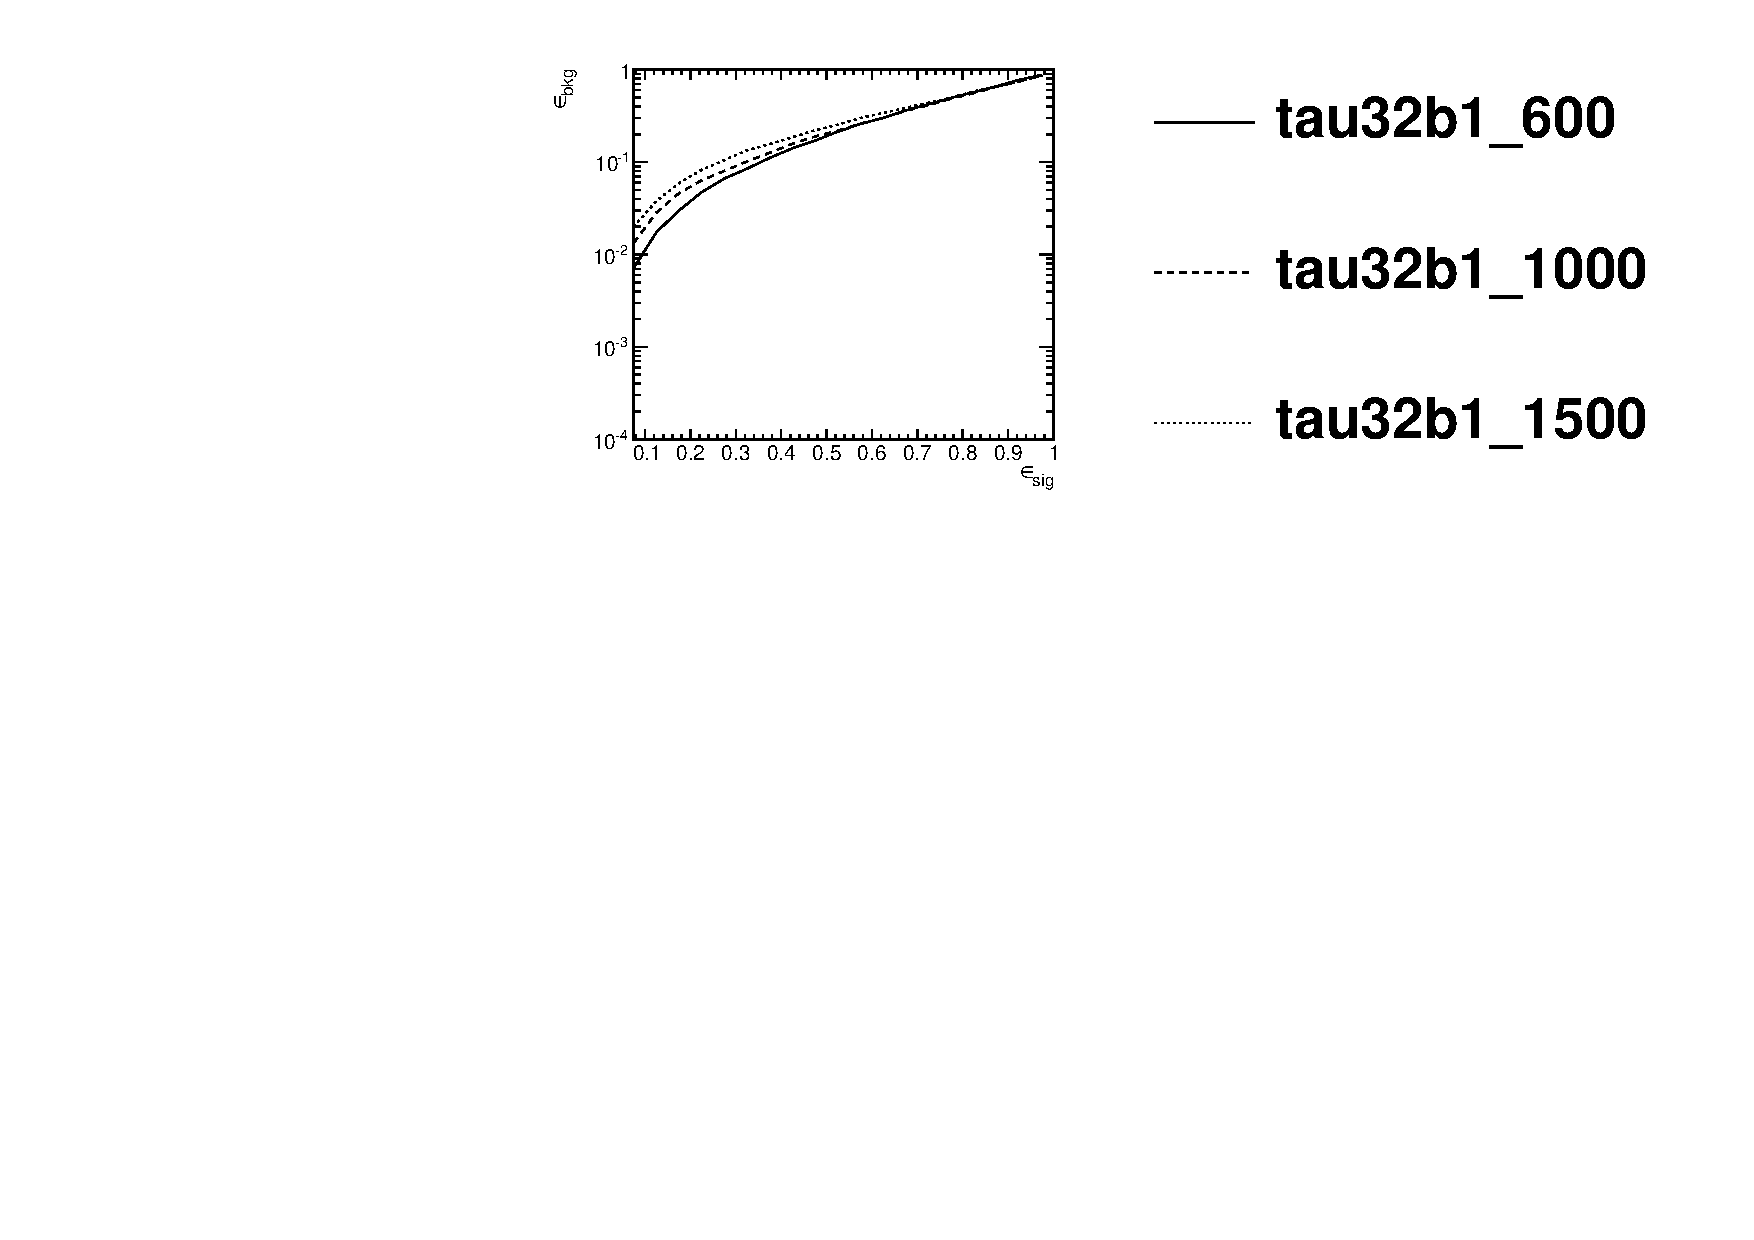
\includegraphics[width=0.48\textwidth]{./Figures/TTagging/pT_compare/Rocs_tau32b1_pTcompare.pdf}}
\subfigure[Mass volatility]{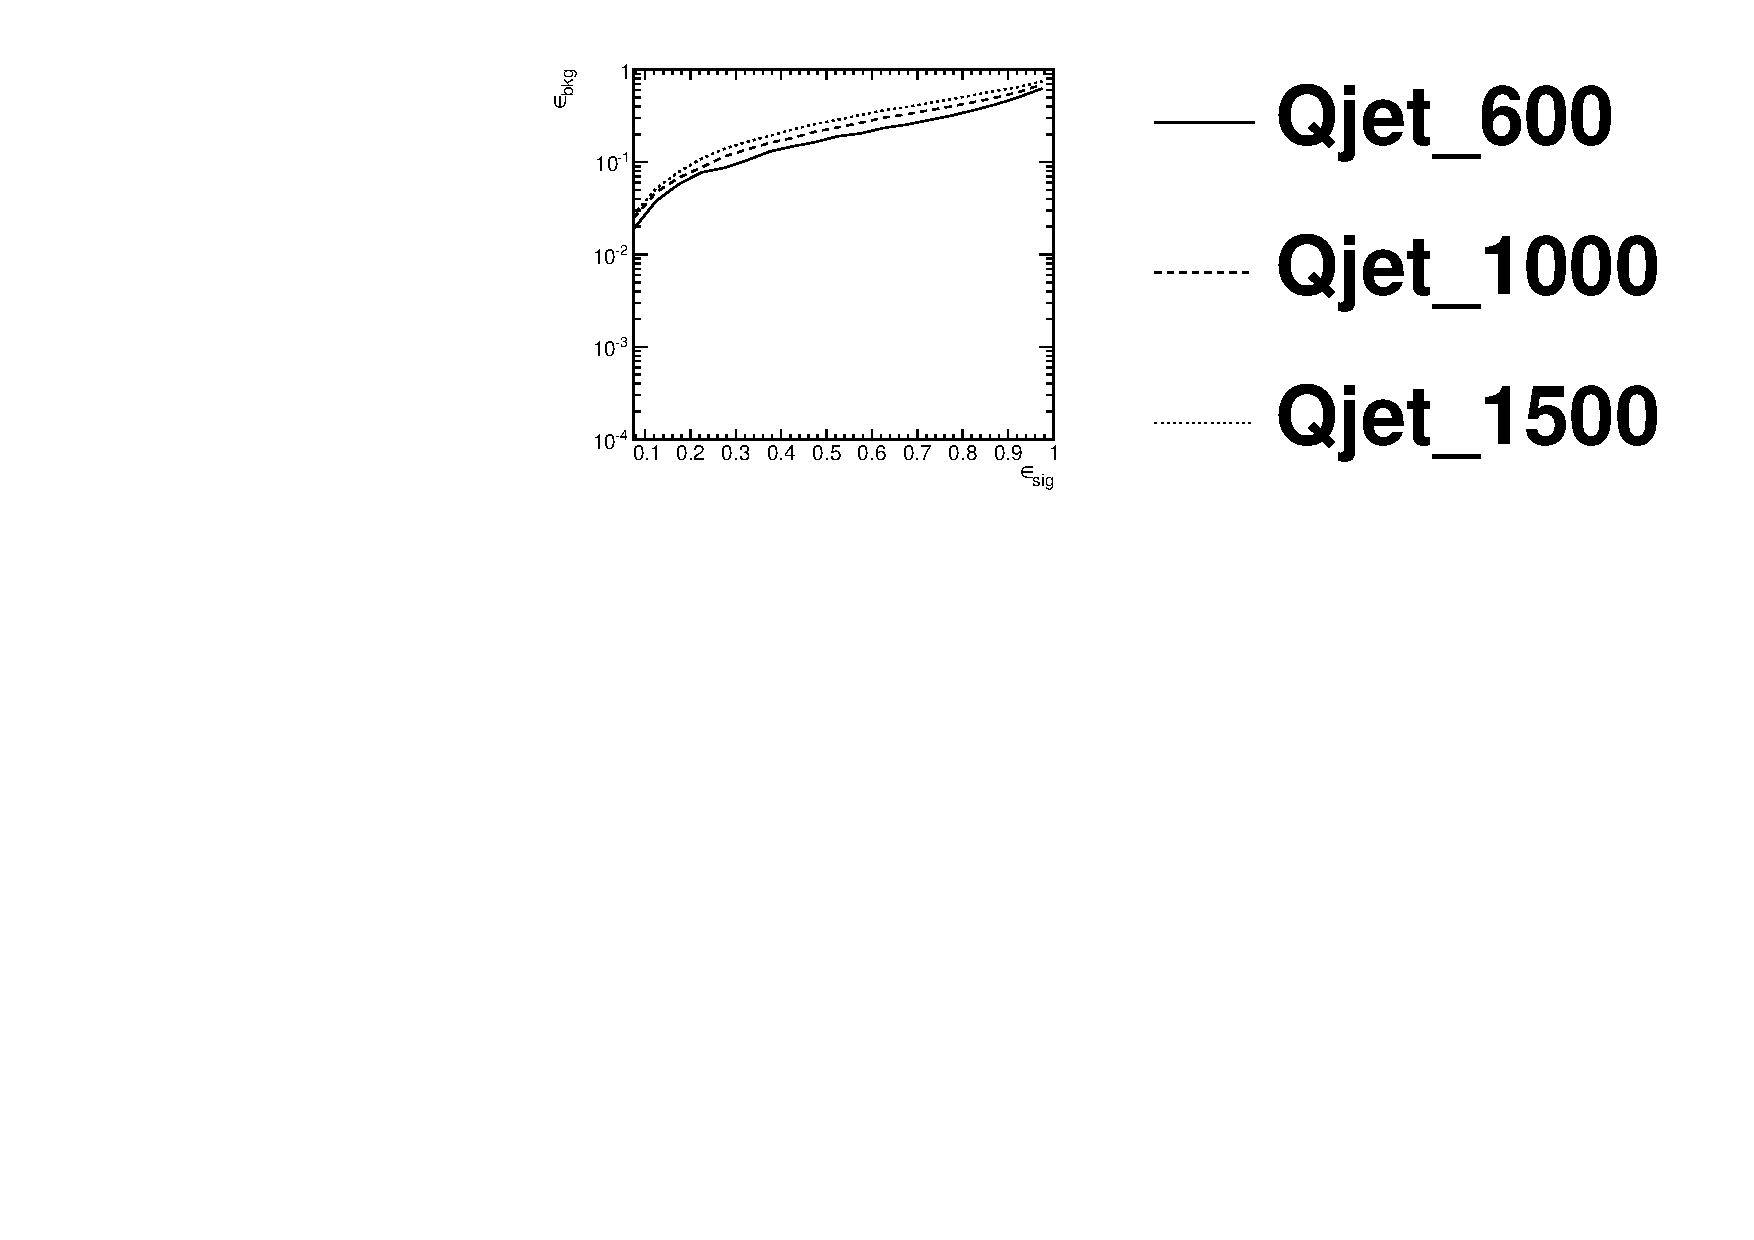
\includegraphics[width=0.48\textwidth]{./Figures/TTagging/pT_compare/Rocs_Qjet_pTcompare.pdf}}
\subfigure[HEPTopTagger]{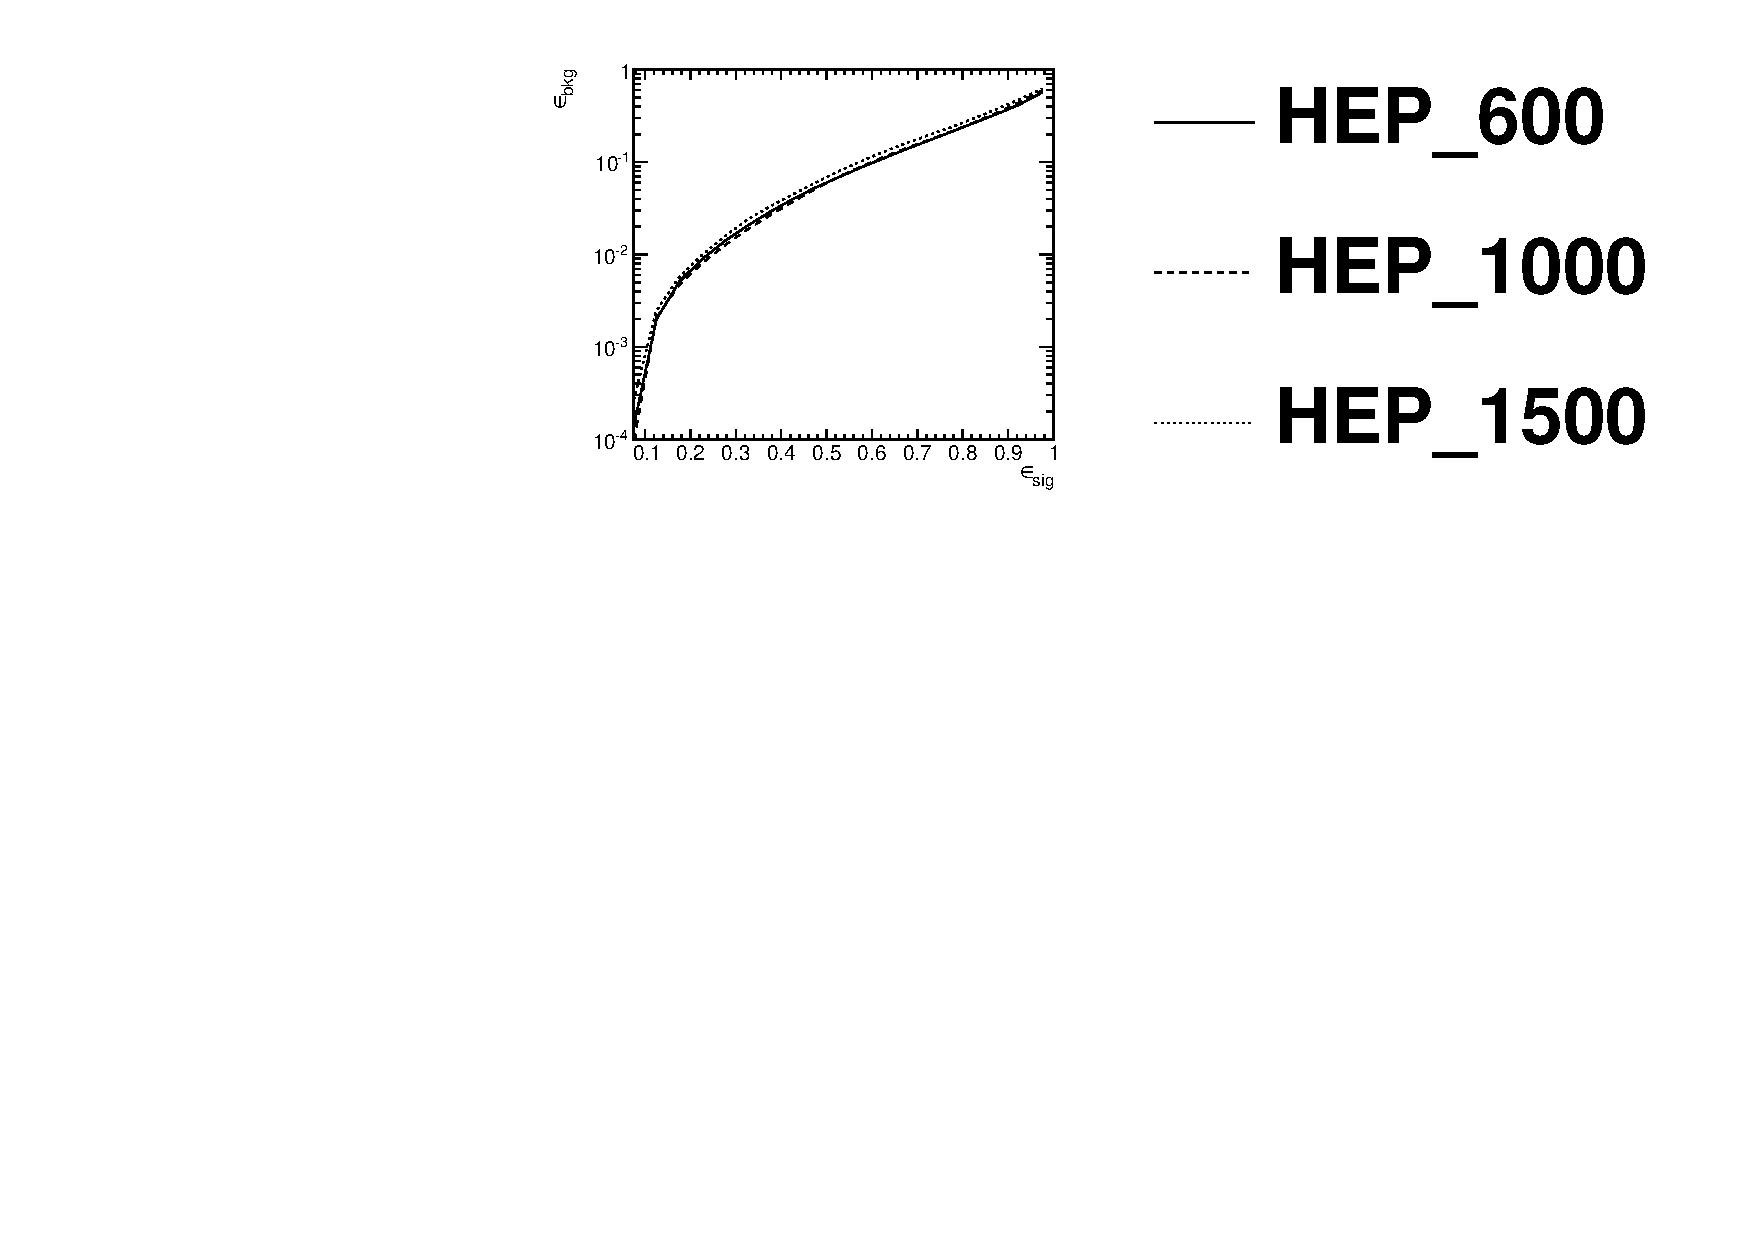
\includegraphics[width=0.48\textwidth]{./Figures/TTagging/pT_compare/Rocs_HEP_pTcompare.pdf}}
\subfigure[Johns Hopkins Tagger]{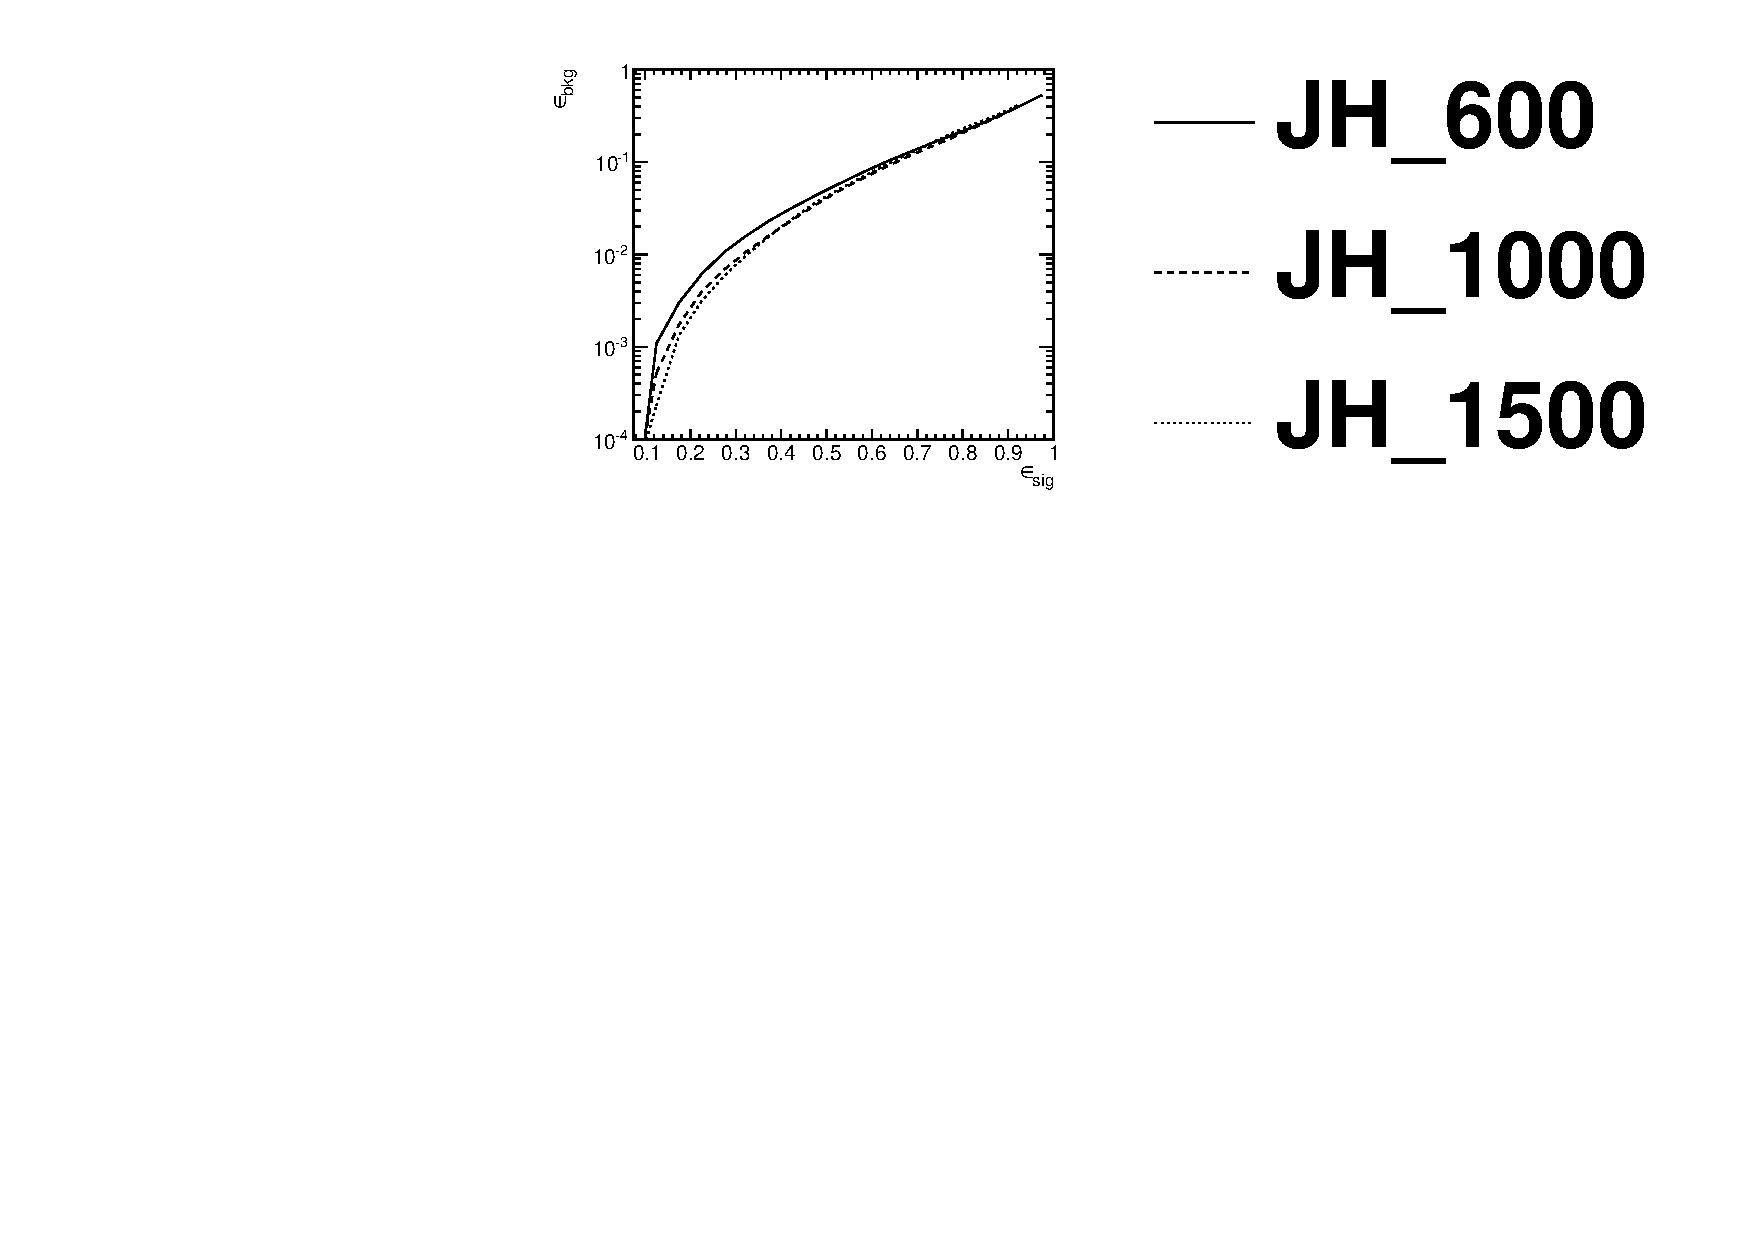
\includegraphics[width=0.48\textwidth]{./Figures/TTagging/pT_compare/Rocs_JH_pTcompare.pdf}}
\subfigure[Trimming]{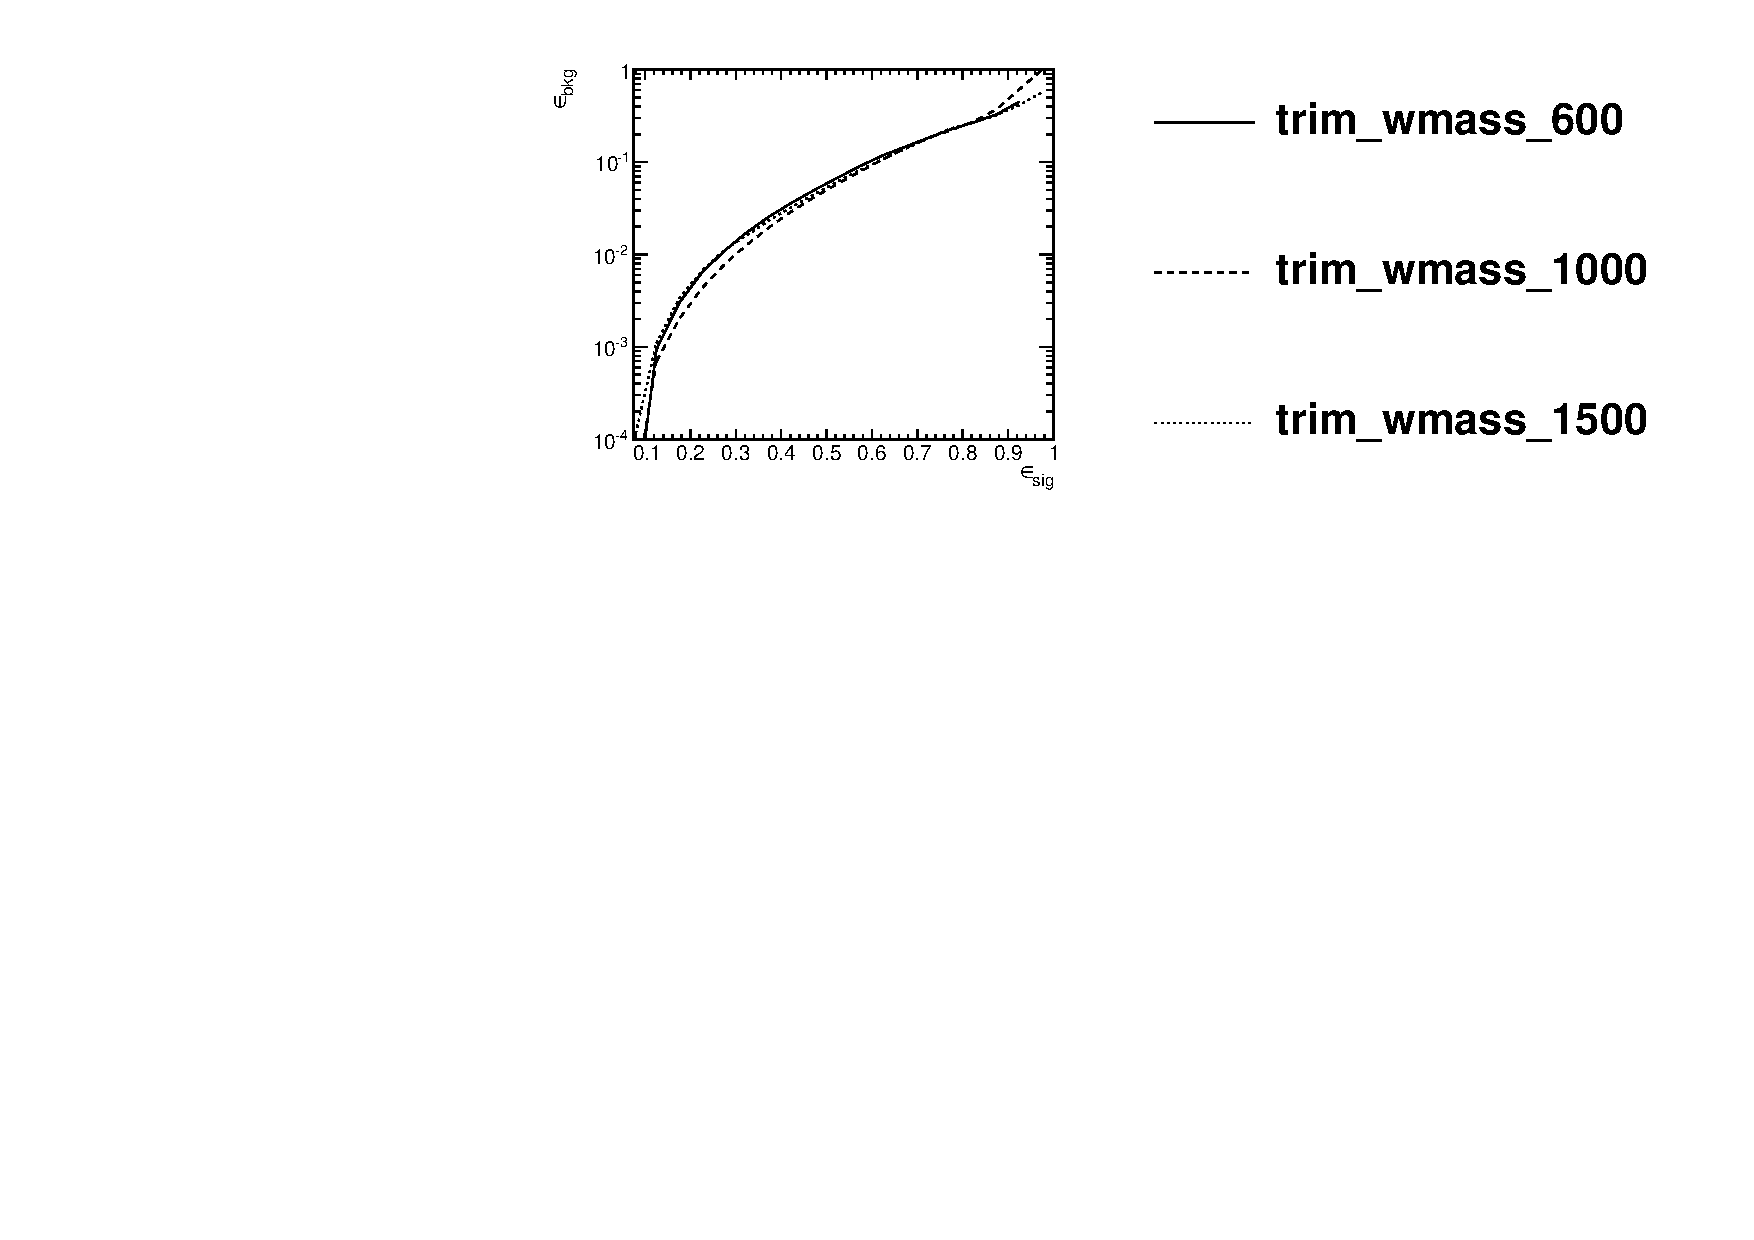
\includegraphics[width=0.48\textwidth]{./Figures/TTagging/pT_compare/Rocs_trim_wmass_pTcompare.pdf}}
\subfigure[Pruning]{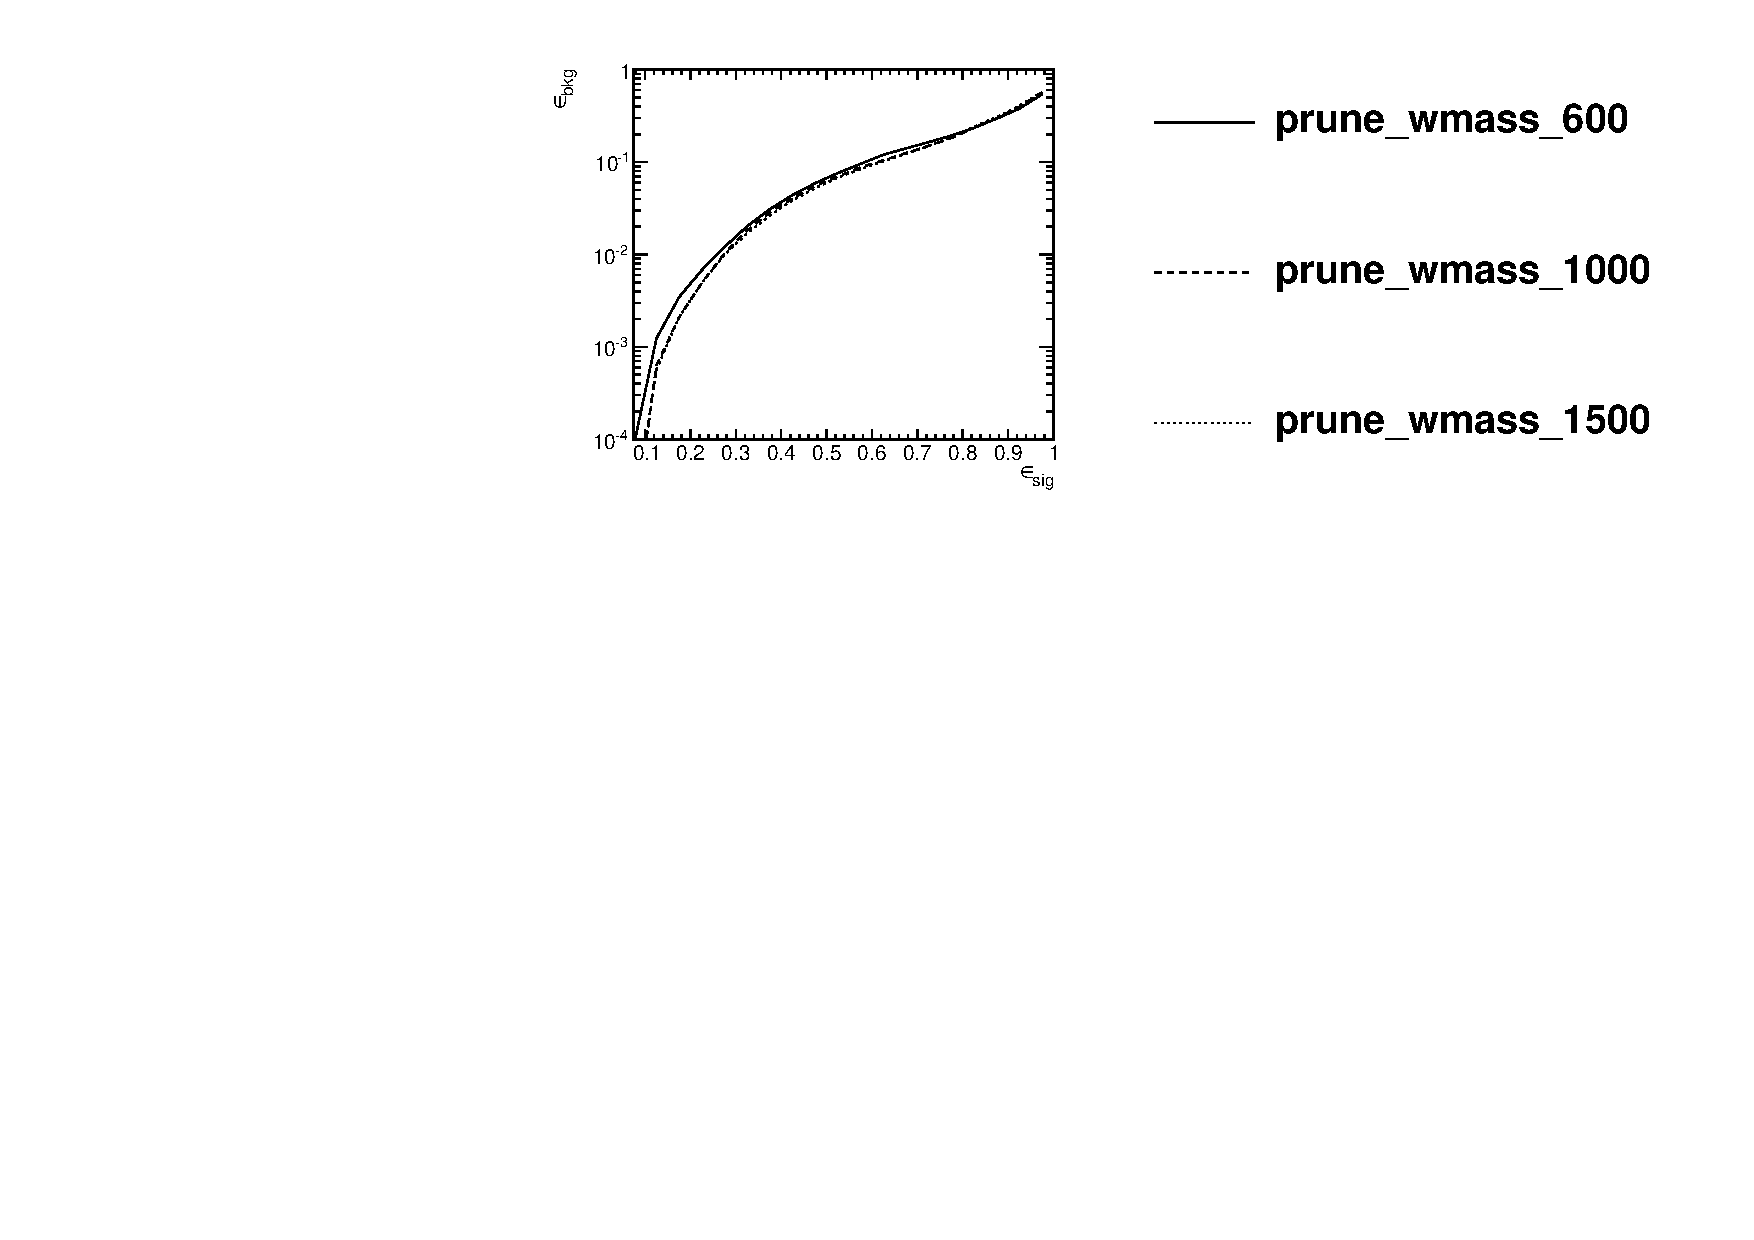
\includegraphics[width=0.48\textwidth]{./Figures/TTagging/pT_compare/Rocs_prune_wmass_pTcompare.pdf}}
\caption{Comparison of tagger and jet shape performance at different \pt using the anti-\kT R=0.8 algorithm.}
\label{fig:ptcomparison_top}
\end{center}
\end{figure*}

\subsection{Direct comparison at different radius}
\begin{figure*}
\begin{center}
\subfigure[C2]{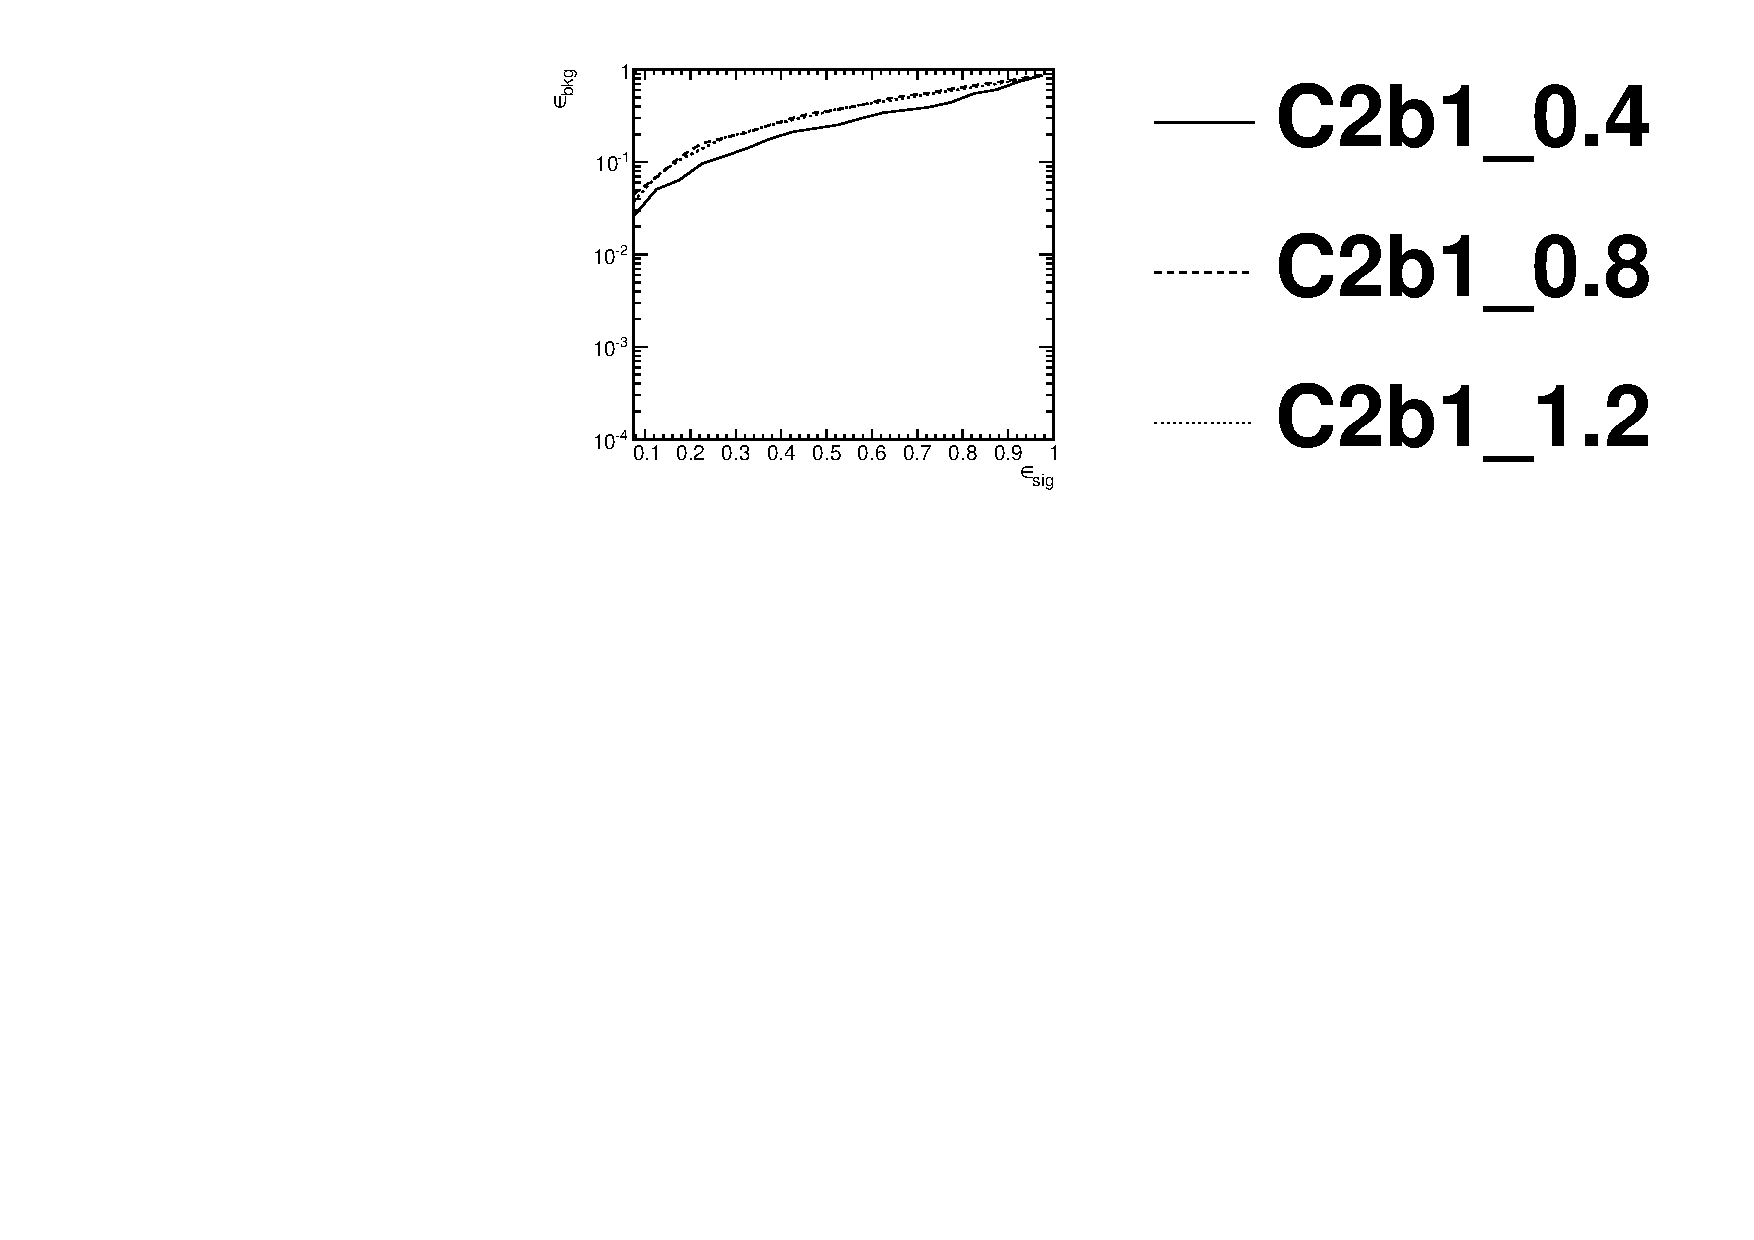
\includegraphics[width=0.48\textwidth]{./Figures/TTagging/R_compare/Rocs_C2b1_Rcompare.pdf}}
\subfigure[C3]{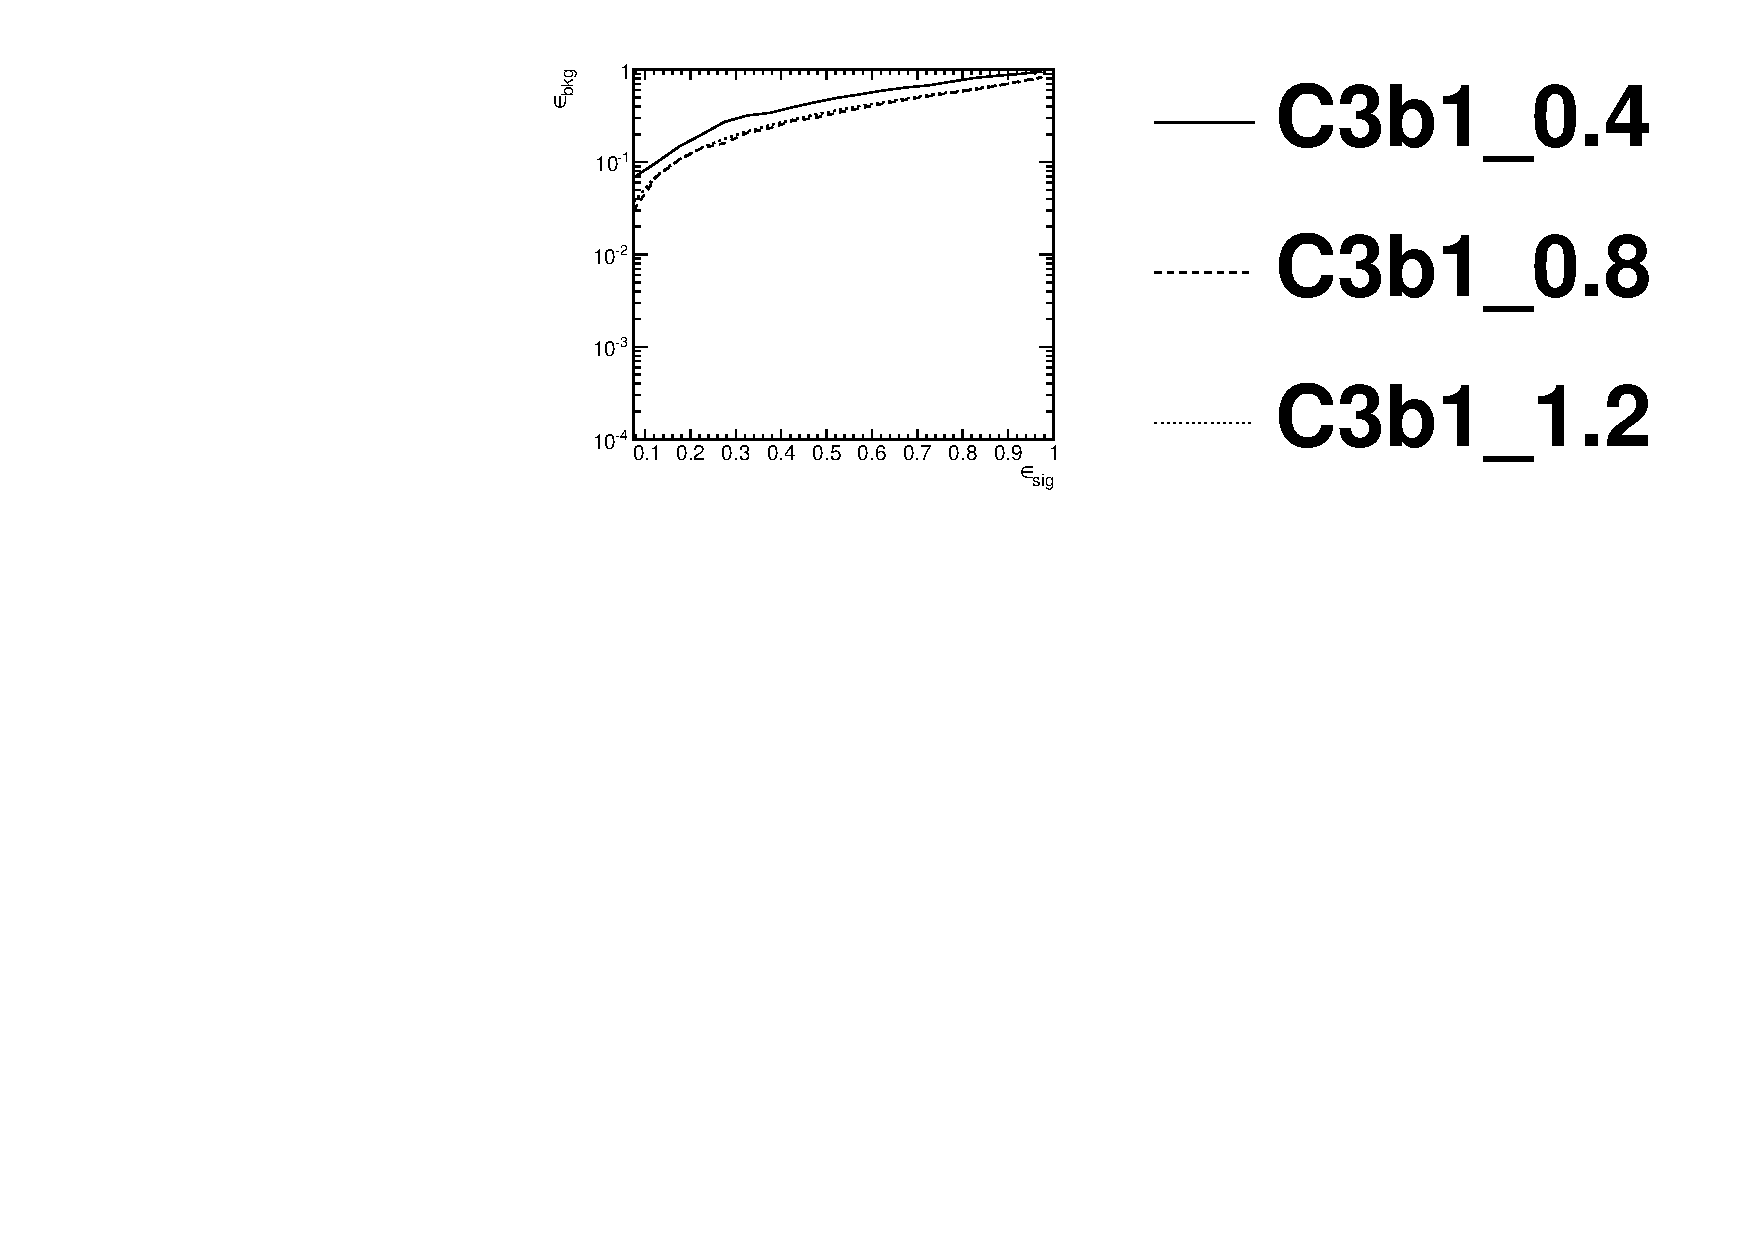
\includegraphics[width=0.48\textwidth]{./Figures/TTagging/R_compare/Rocs_C3b1_Rcompare.pdf}}
\subfigure[$\tau_{21}$]{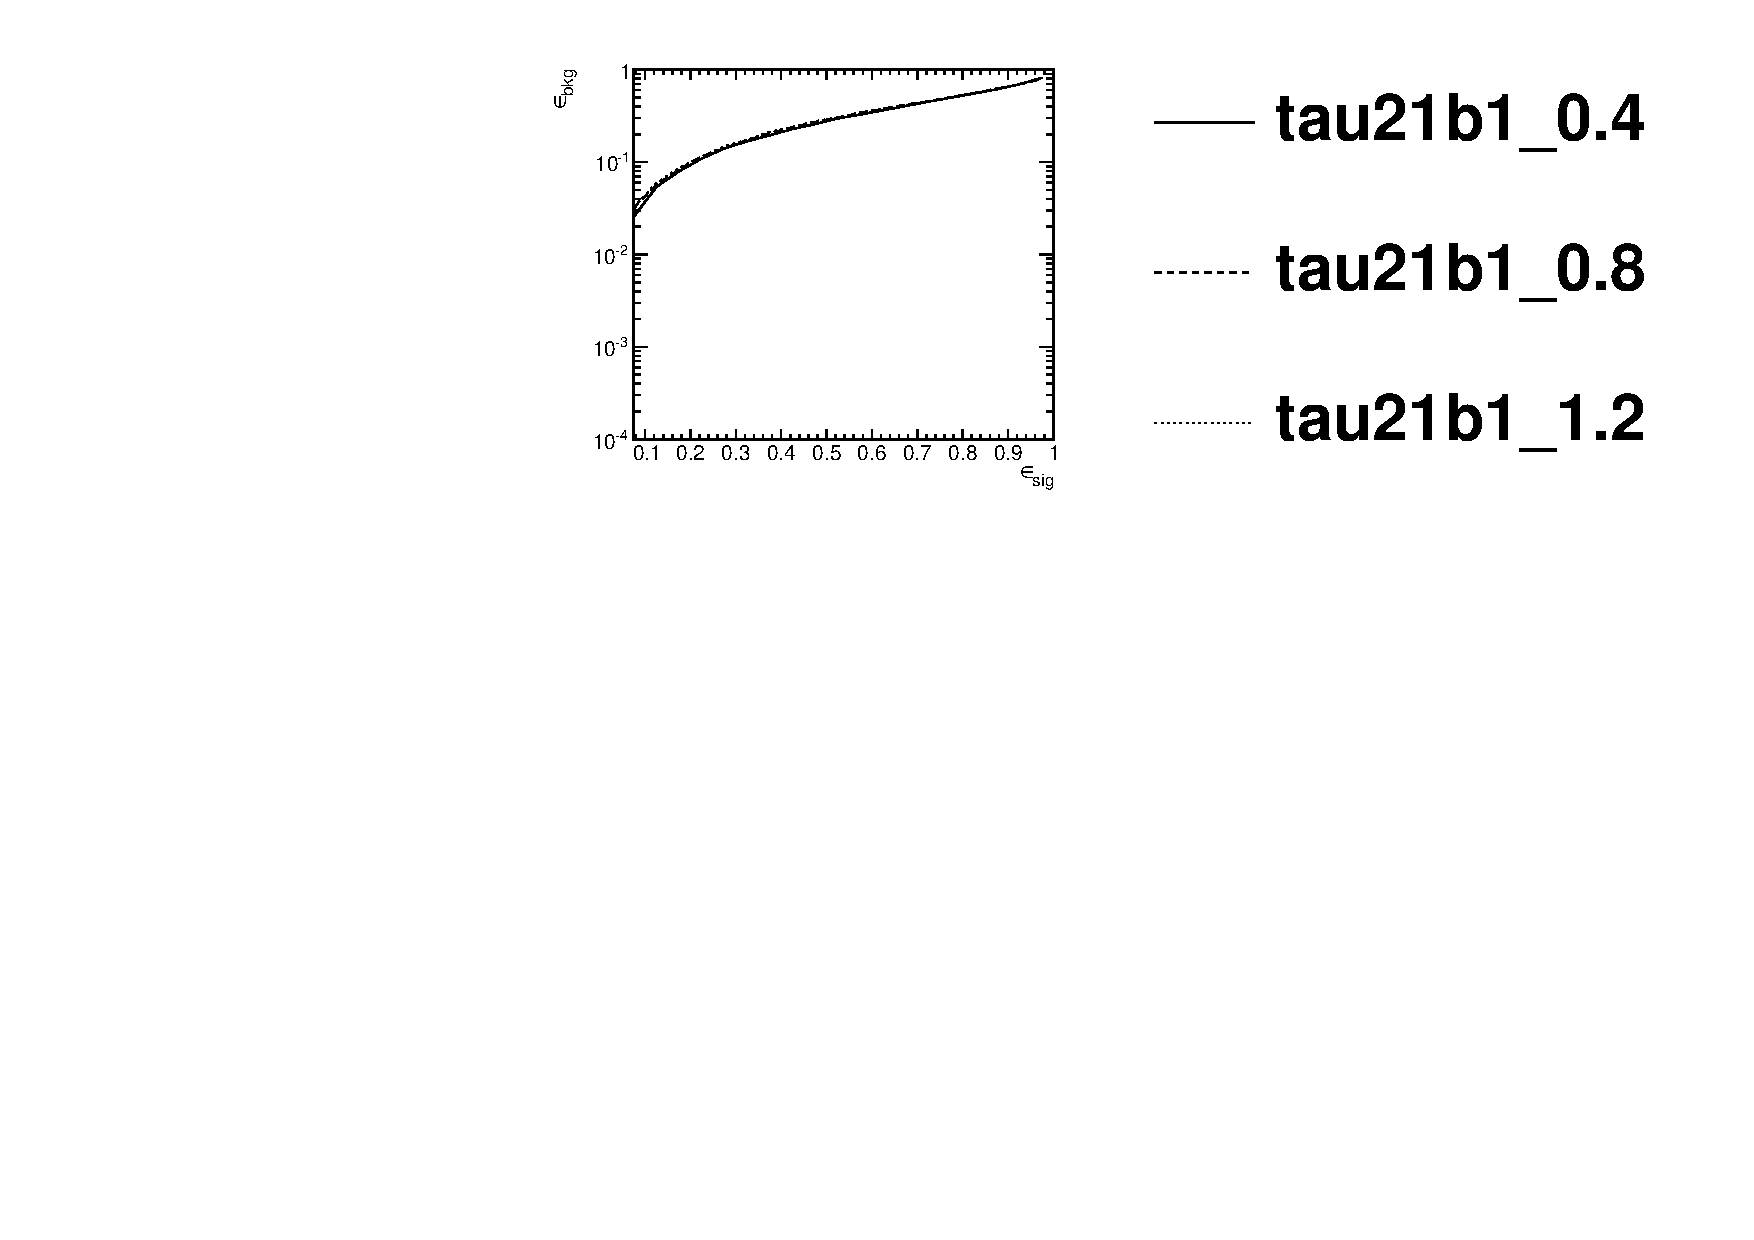
\includegraphics[width=0.48\textwidth]{./Figures/TTagging/R_compare/Rocs_tau21b1_Rcompare.pdf}}
\subfigure[$\tau_{32}$]{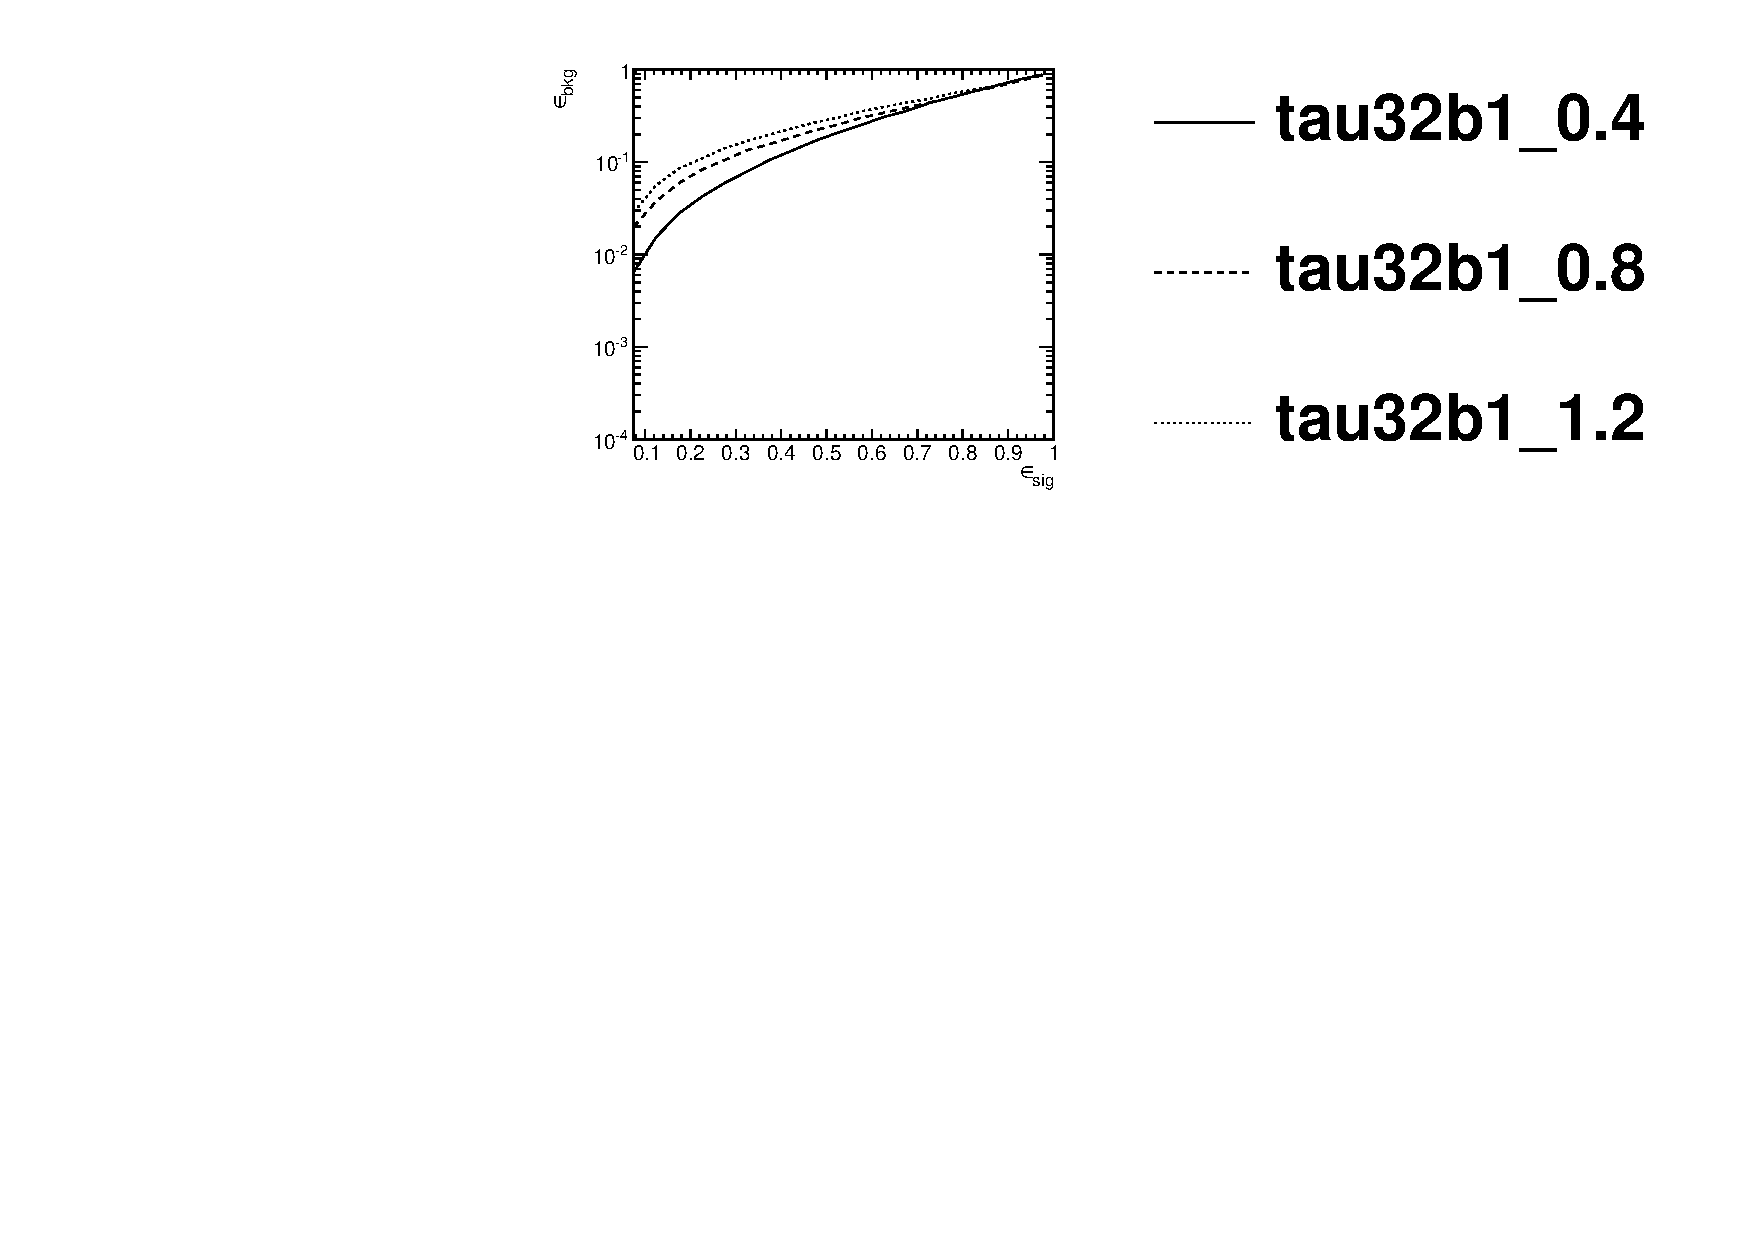
\includegraphics[width=0.48\textwidth]{./Figures/TTagging/R_compare/Rocs_tau32b1_Rcompare.pdf}}
\subfigure[Mass volatility]{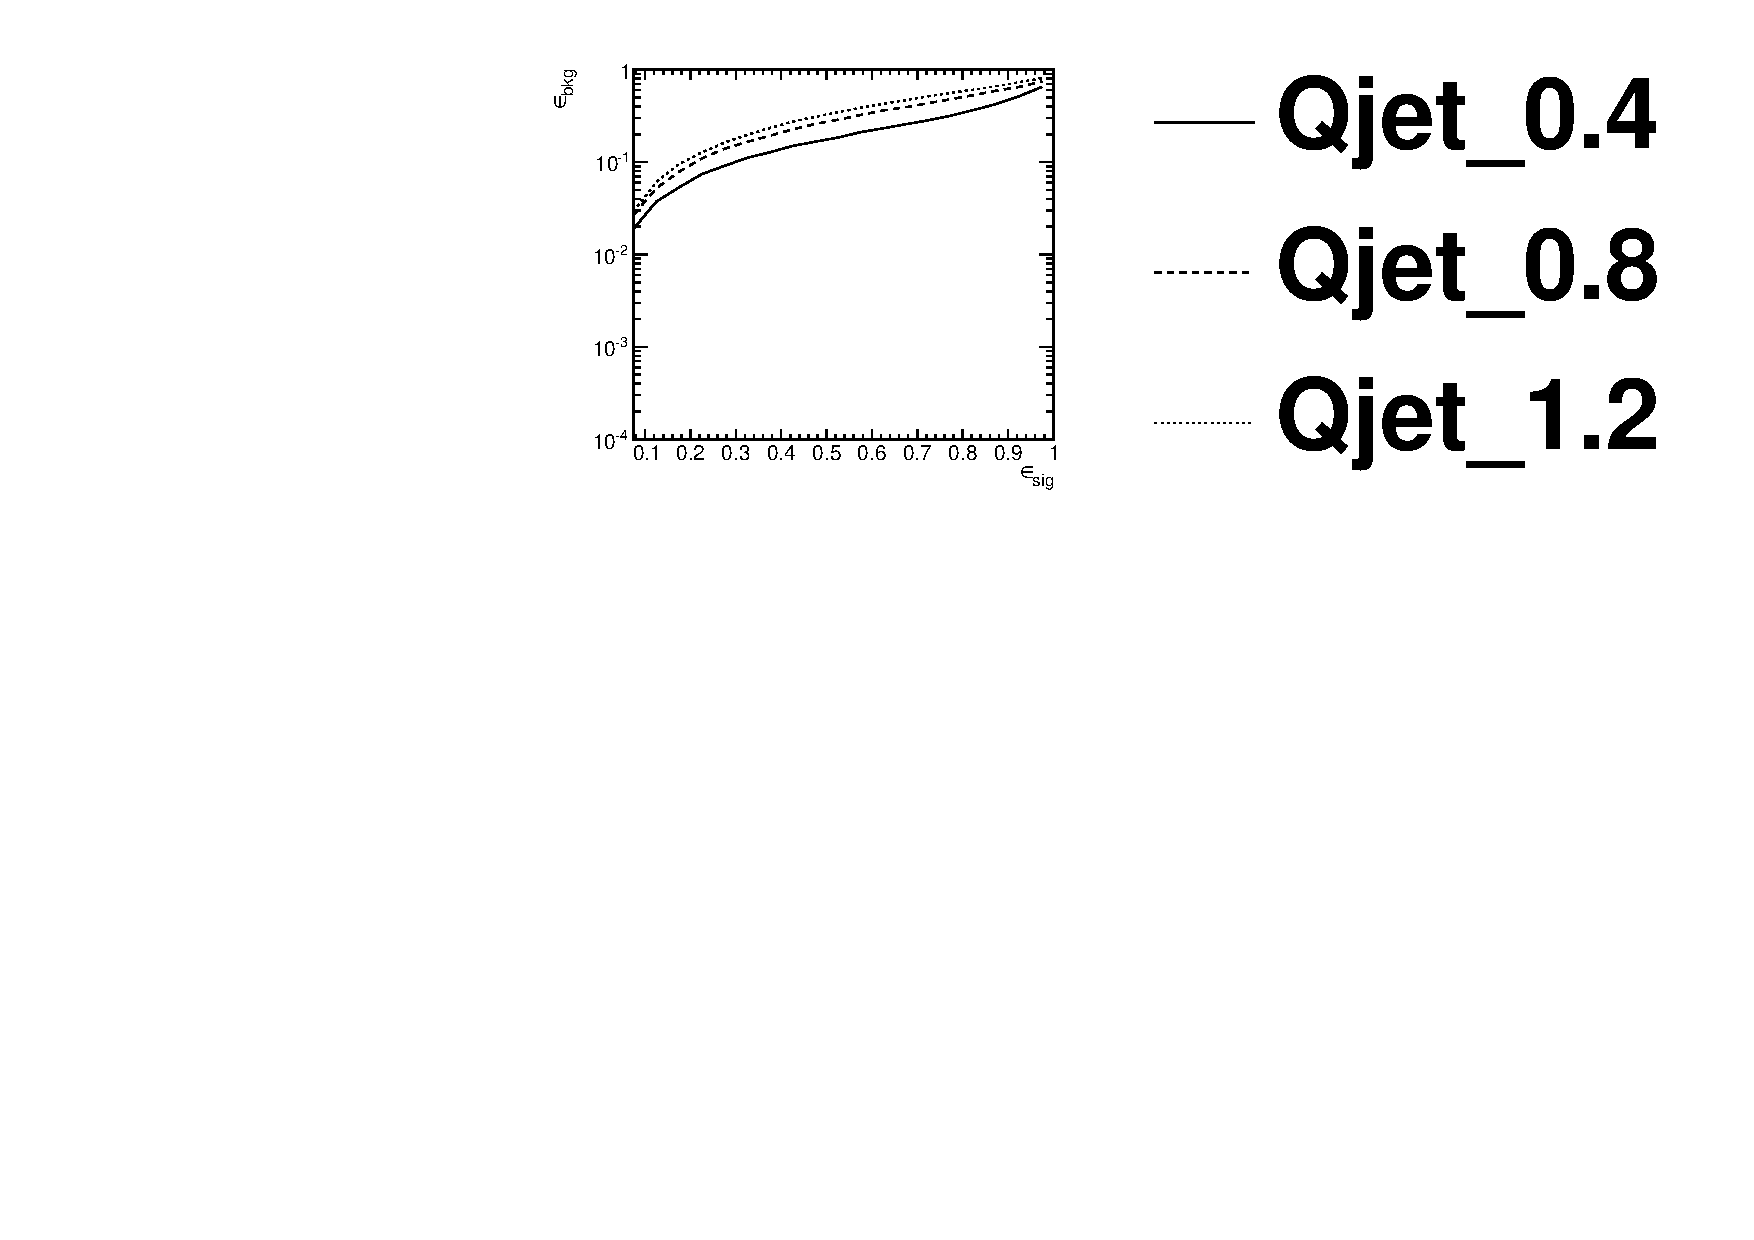
\includegraphics[width=0.48\textwidth]{./Figures/TTagging/R_compare/Rocs_Qjet_Rcompare.pdf}}
\subfigure[HEPTopTagger]{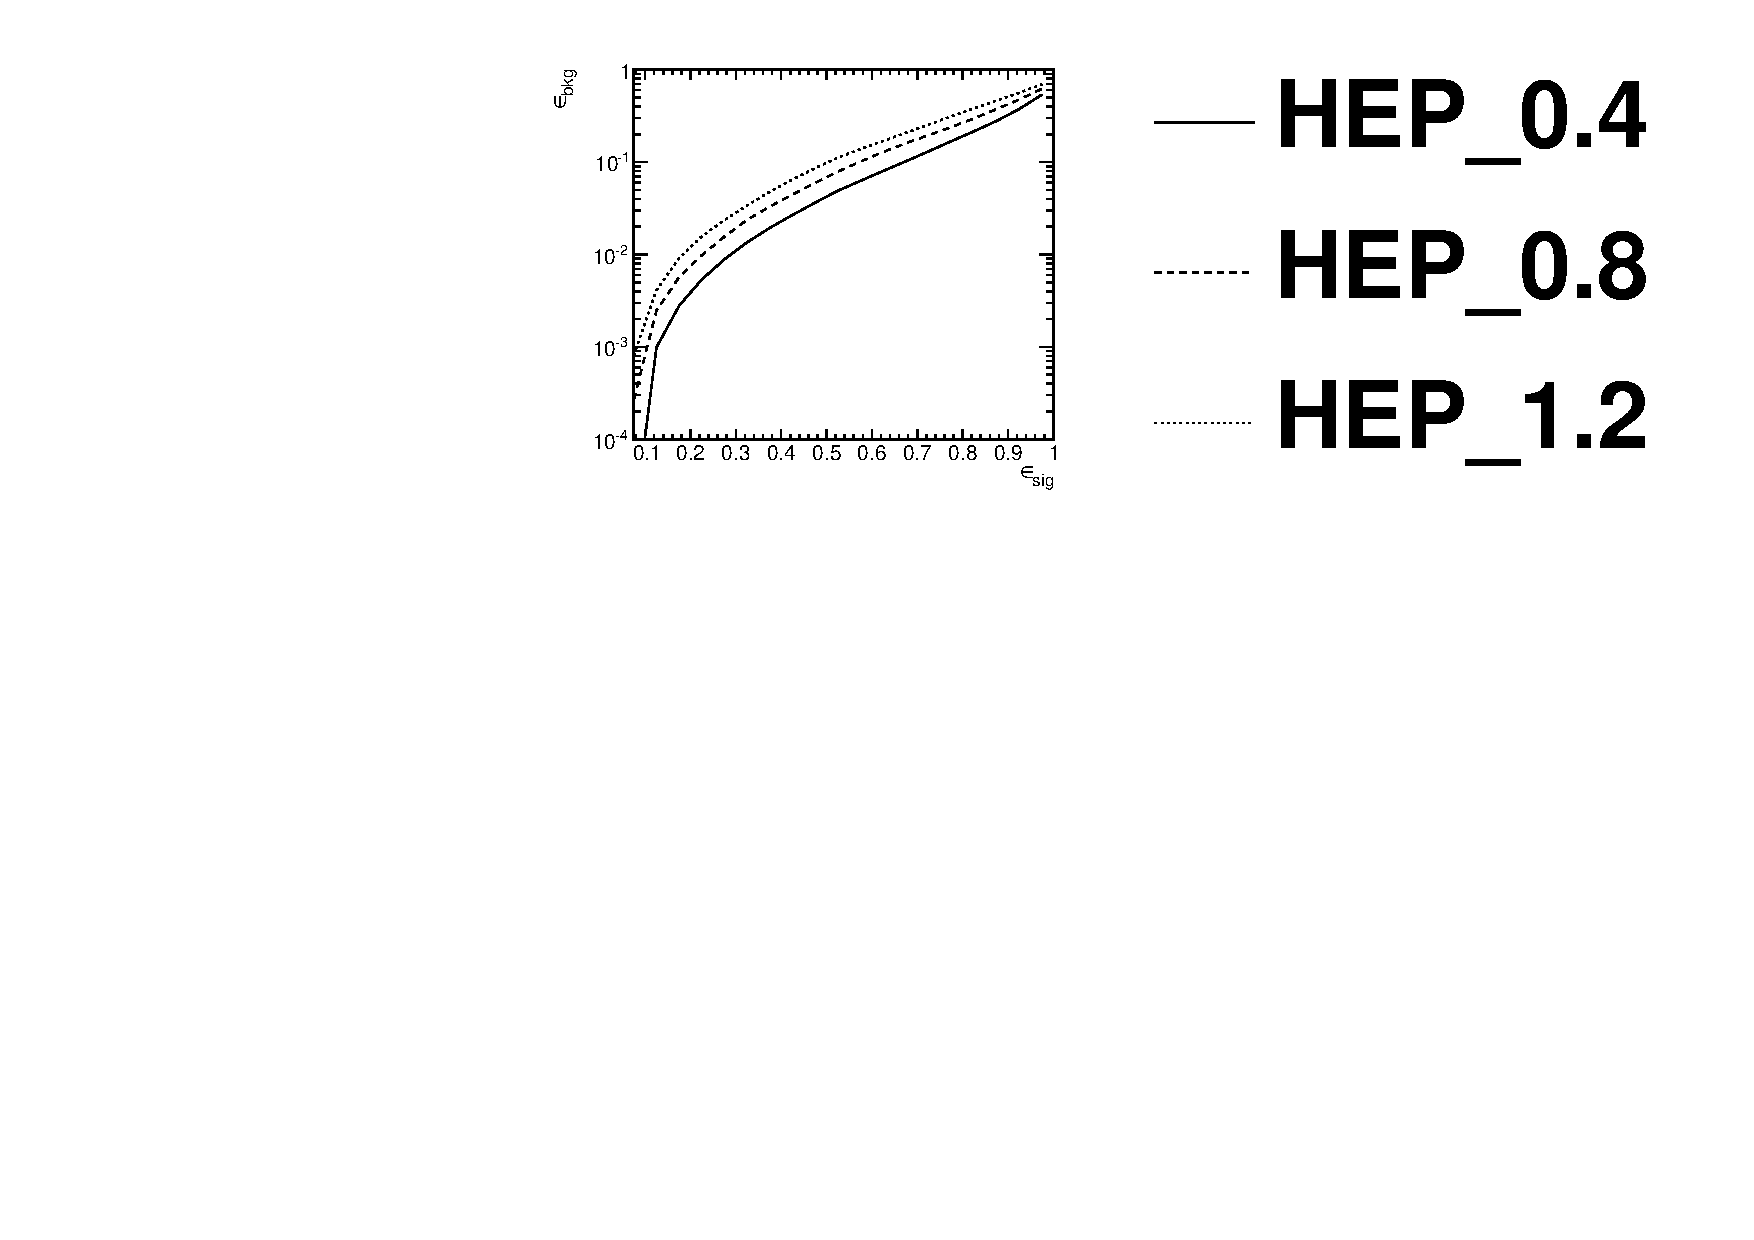
\includegraphics[width=0.48\textwidth]{./Figures/TTagging/R_compare/Rocs_HEP_Rcompare.pdf}}
\subfigure[Johns Hopkins Tagger]{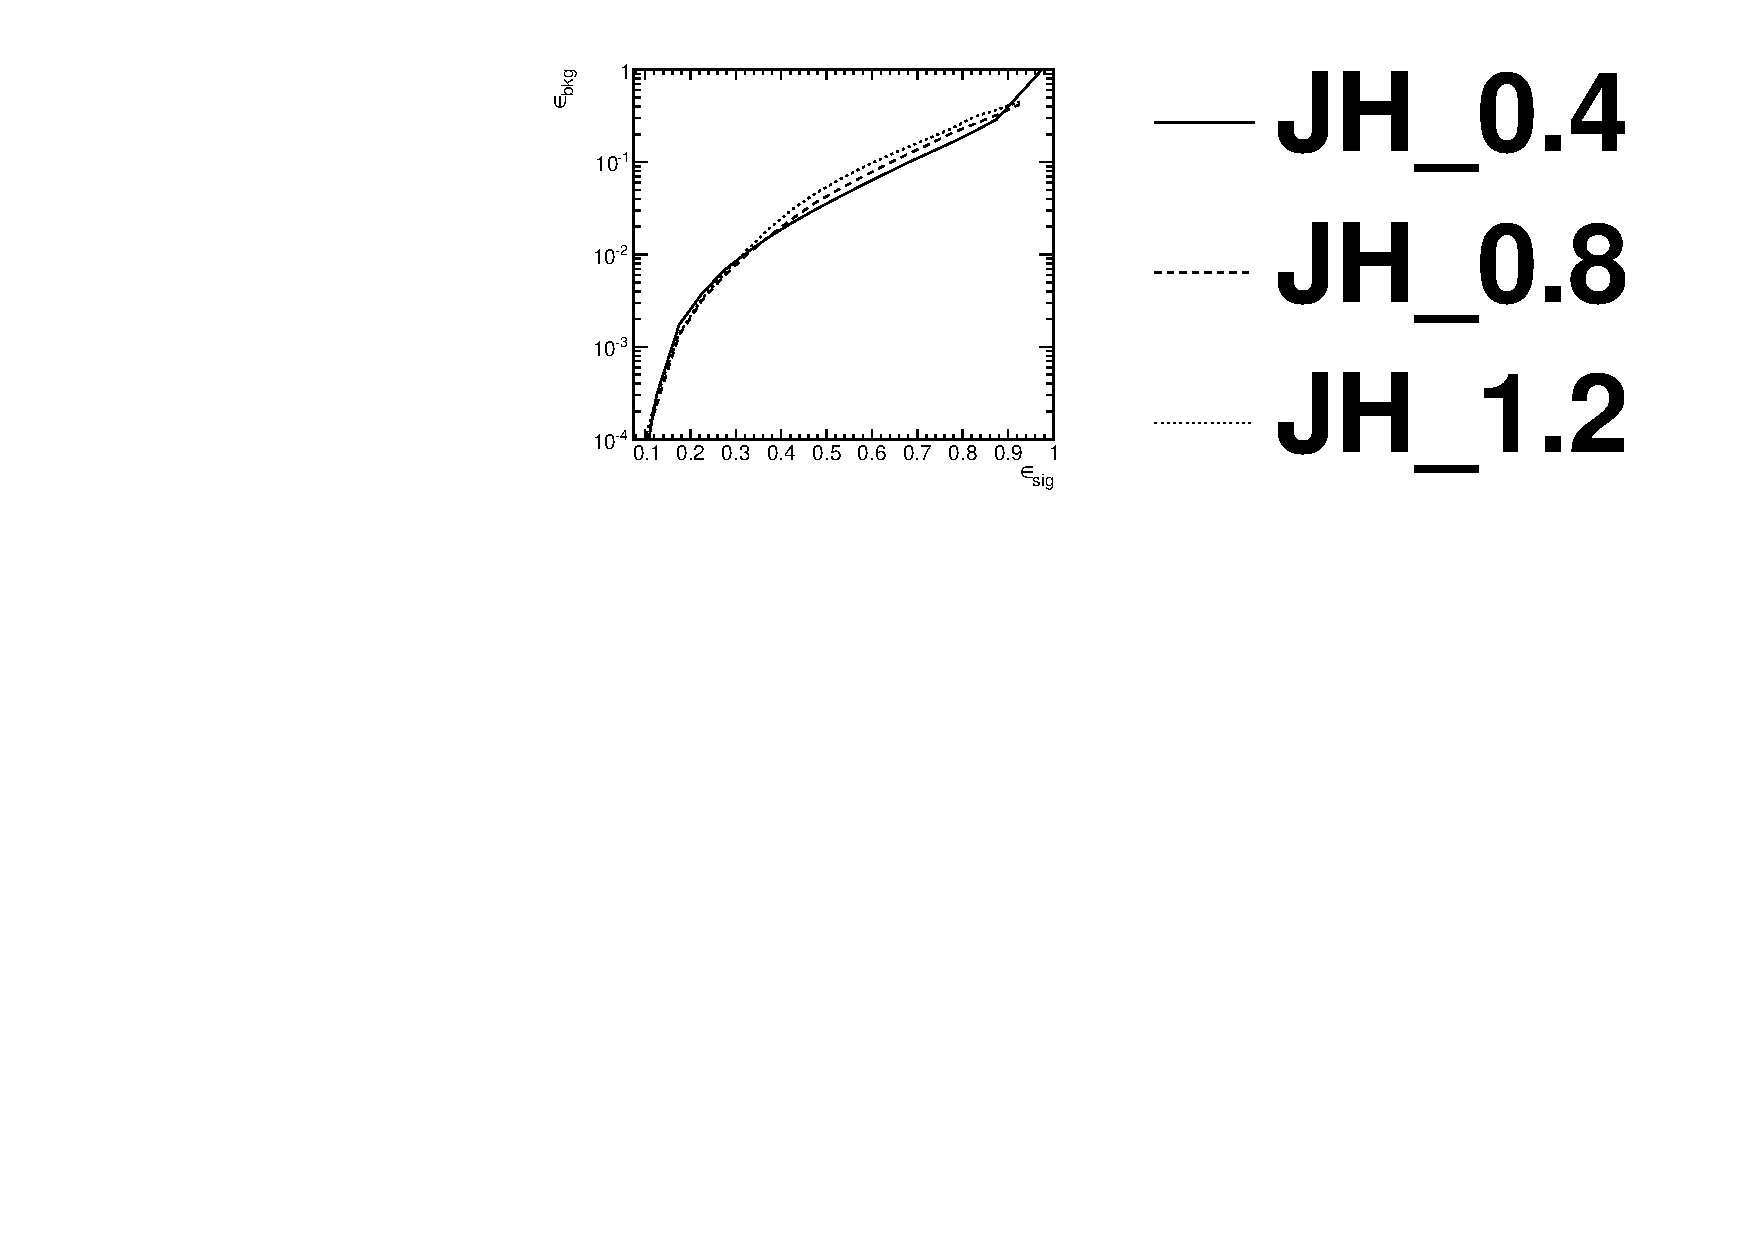
\includegraphics[width=0.48\textwidth]{./Figures/TTagging/R_compare/Rocs_JH_Rcompare.pdf}}
\subfigure[Trimming]{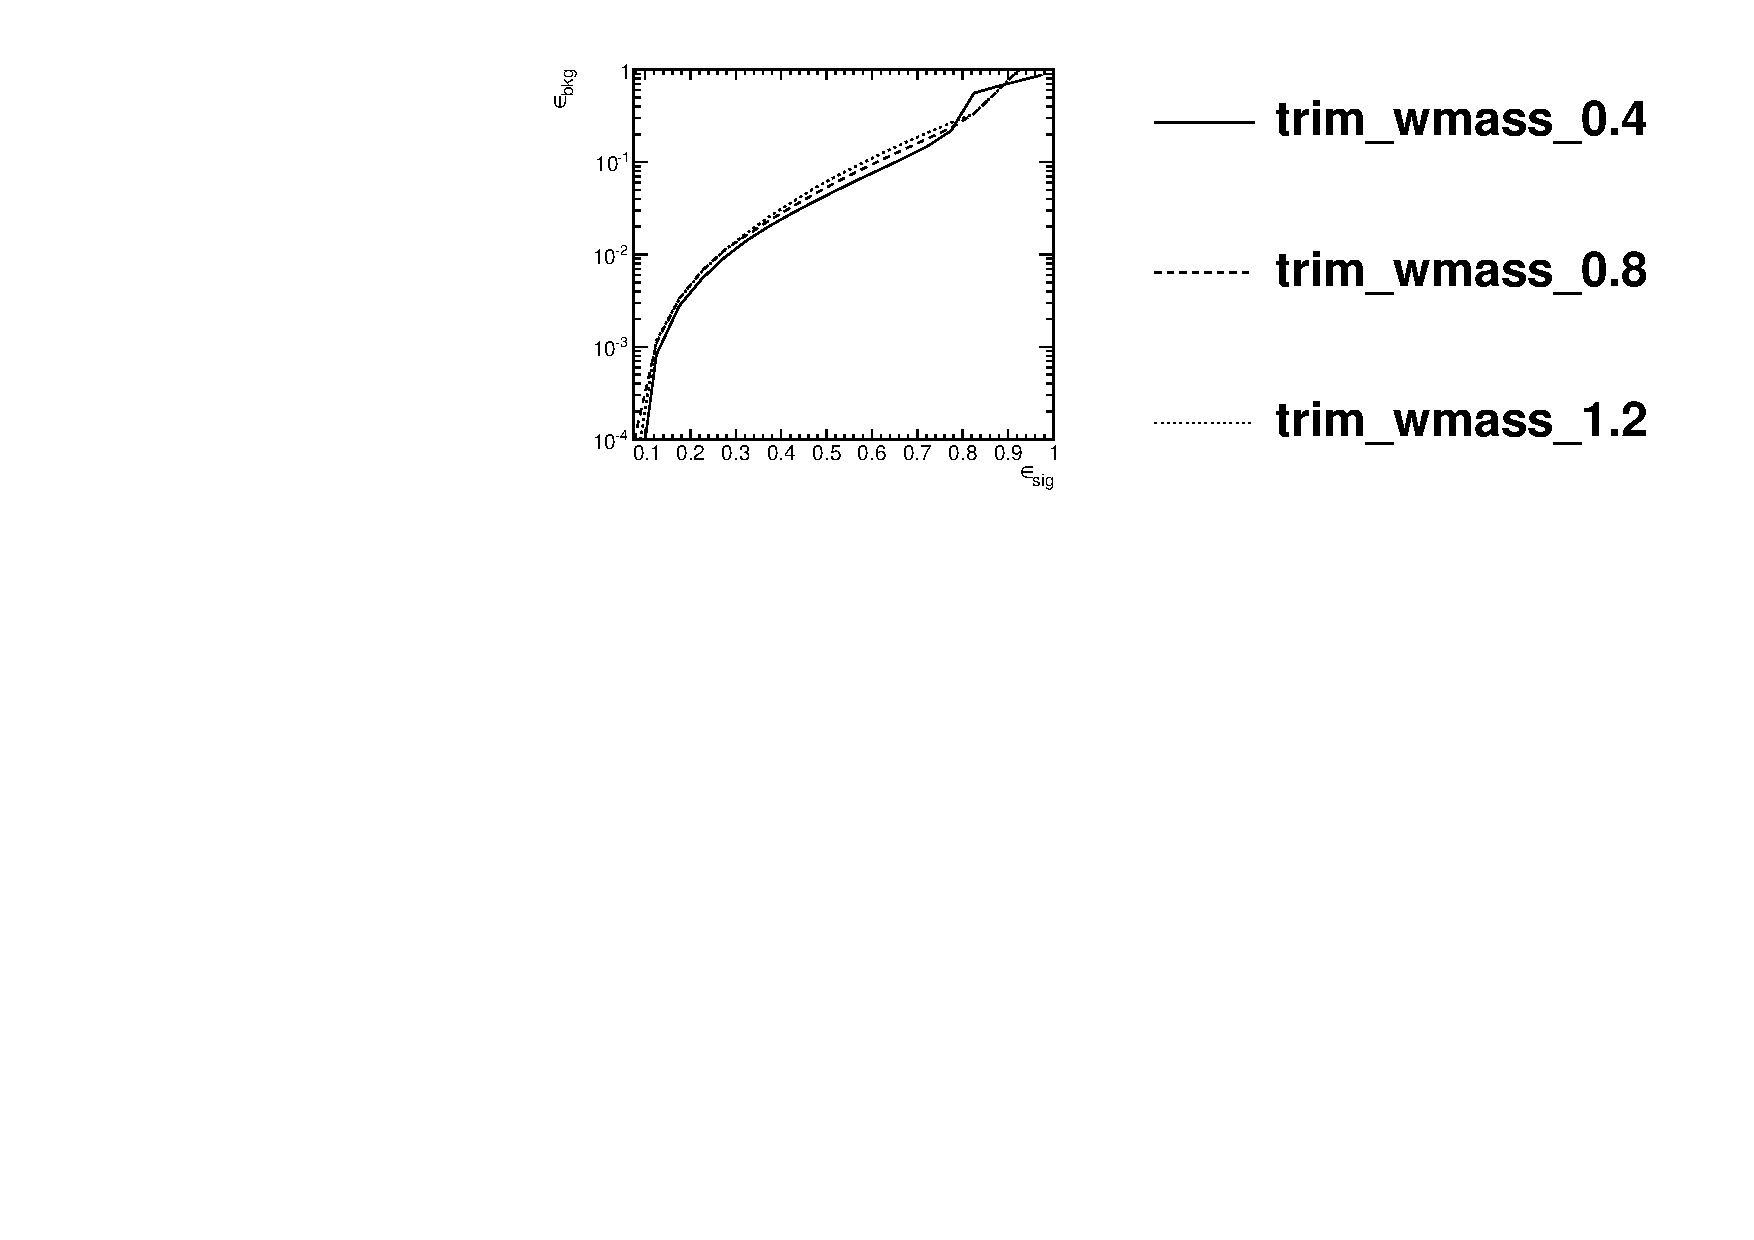
\includegraphics[width=0.48\textwidth]{./Figures/TTagging/R_compare/Rocs_trim_wmass_Rcompare.pdf}}
\subfigure[Pruning]{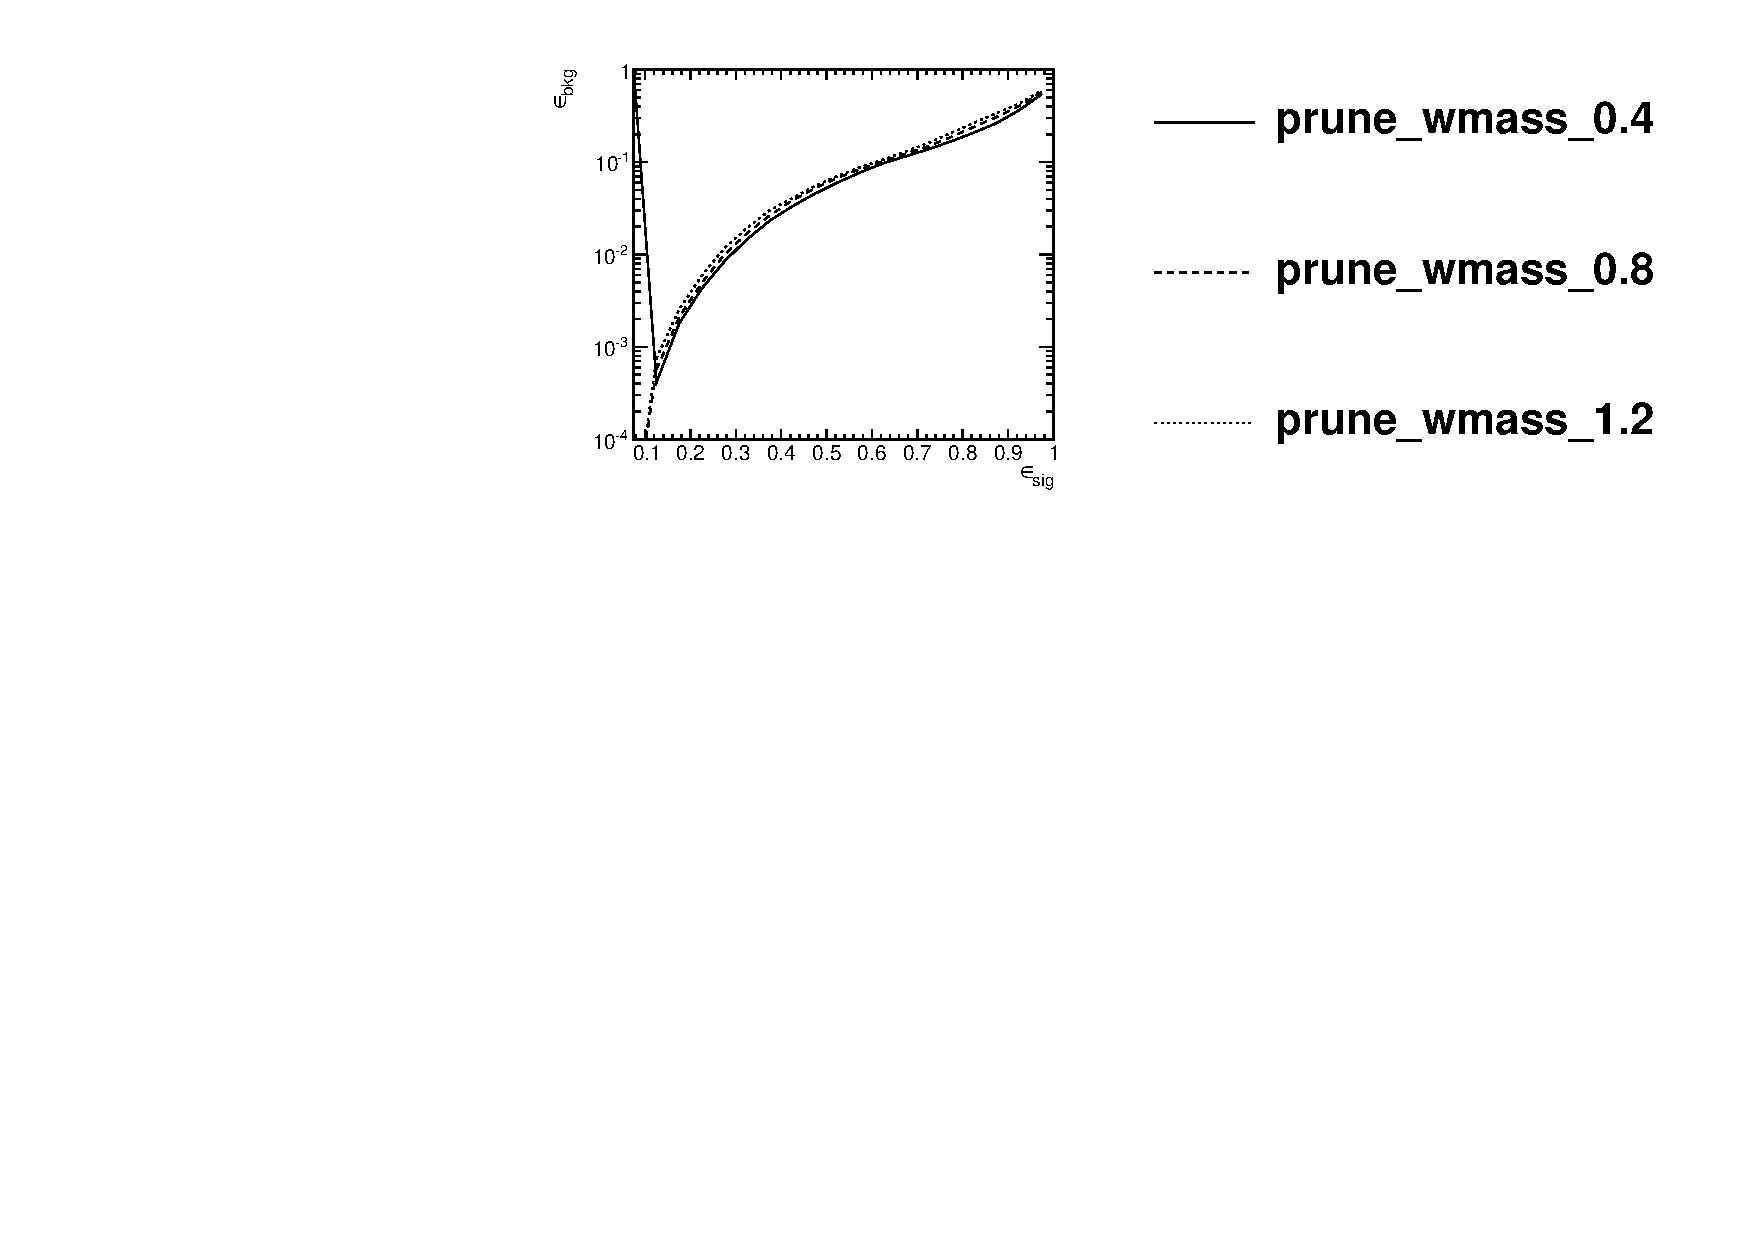
\includegraphics[width=0.48\textwidth]{./Figures/TTagging/R_compare/Rocs_prune_wmass_Rcompare.pdf}}
\caption{Comparison of tagger and jet shape performance at different radius at \pt = 1.5 TeV.}
\label{fig:Rcomparison_top}
\end{center}
\end{figure*}
